\documentclass[twoside]{book}

% Packages required by doxygen
\usepackage{fixltx2e}
\usepackage{calc}
\usepackage{doxygen}
\usepackage[export]{adjustbox} % also loads graphicx
\usepackage{graphicx}
\usepackage[utf8]{inputenc}
\usepackage{makeidx}
\usepackage{multicol}
\usepackage{multirow}
\PassOptionsToPackage{warn}{textcomp}
\usepackage{textcomp}
\usepackage[nointegrals]{wasysym}
\usepackage[table]{xcolor}

% Font selection
\usepackage[T1]{fontenc}
\usepackage[scaled=.90]{helvet}
\usepackage{courier}
\usepackage{amssymb}
\usepackage{sectsty}
\renewcommand{\familydefault}{\sfdefault}
\allsectionsfont{%
  \fontseries{bc}\selectfont%
  \color{darkgray}%
}
\renewcommand{\DoxyLabelFont}{%
  \fontseries{bc}\selectfont%
  \color{darkgray}%
}
\newcommand{\+}{\discretionary{\mbox{\scriptsize$\hookleftarrow$}}{}{}}

% Page & text layout
\usepackage{geometry}
\geometry{%
  a4paper,%
  top=2.5cm,%
  bottom=2.5cm,%
  left=2.5cm,%
  right=2.5cm%
}
\tolerance=750
\hfuzz=15pt
\hbadness=750
\setlength{\emergencystretch}{15pt}
\setlength{\parindent}{0cm}
\setlength{\parskip}{3ex plus 2ex minus 2ex}
\makeatletter
\renewcommand{\paragraph}{%
  \@startsection{paragraph}{4}{0ex}{-1.0ex}{1.0ex}{%
    \normalfont\normalsize\bfseries\SS@parafont%
  }%
}
\renewcommand{\subparagraph}{%
  \@startsection{subparagraph}{5}{0ex}{-1.0ex}{1.0ex}{%
    \normalfont\normalsize\bfseries\SS@subparafont%
  }%
}
\makeatother

% Headers & footers
\usepackage{fancyhdr}
\pagestyle{fancyplain}
\fancyhead[LE]{\fancyplain{}{\bfseries\thepage}}
\fancyhead[CE]{\fancyplain{}{}}
\fancyhead[RE]{\fancyplain{}{\bfseries\leftmark}}
\fancyhead[LO]{\fancyplain{}{\bfseries\rightmark}}
\fancyhead[CO]{\fancyplain{}{}}
\fancyhead[RO]{\fancyplain{}{\bfseries\thepage}}
\fancyfoot[LE]{\fancyplain{}{}}
\fancyfoot[CE]{\fancyplain{}{}}
\fancyfoot[RE]{\fancyplain{}{\bfseries\scriptsize Generated by Doxygen }}
\fancyfoot[LO]{\fancyplain{}{\bfseries\scriptsize Generated by Doxygen }}
\fancyfoot[CO]{\fancyplain{}{}}
\fancyfoot[RO]{\fancyplain{}{}}
\renewcommand{\footrulewidth}{0.4pt}
\renewcommand{\chaptermark}[1]{%
  \markboth{#1}{}%
}
\renewcommand{\sectionmark}[1]{%
  \markright{\thesection\ #1}%
}

% Indices & bibliography
\usepackage{natbib}
\usepackage[titles]{tocloft}
\setcounter{tocdepth}{3}
\setcounter{secnumdepth}{5}
\makeindex

% Hyperlinks (required, but should be loaded last)
\usepackage{ifpdf}
\ifpdf
  \usepackage[pdftex,pagebackref=true]{hyperref}
\else
  \usepackage[ps2pdf,pagebackref=true]{hyperref}
\fi
\hypersetup{%
  colorlinks=true,%
  linkcolor=blue,%
  citecolor=blue,%
  unicode%
}

% Custom commands
\newcommand{\clearemptydoublepage}{%
  \newpage{\pagestyle{empty}\cleardoublepage}%
}

\usepackage{caption}
\captionsetup{labelsep=space,justification=centering,font={bf},singlelinecheck=off,skip=4pt,position=top}

%===== C O N T E N T S =====

\begin{document}

% Titlepage & ToC
\hypersetup{pageanchor=false,
             bookmarksnumbered=true,
             pdfencoding=unicode
            }
\pagenumbering{roman}
\begin{titlepage}
\vspace*{7cm}
\begin{center}%
{\Large eigen\+\_\+state\+\_\+space\+\_\+systems }\\
\vspace*{1cm}
{\large Generated by Doxygen 1.8.11}\\
\end{center}
\end{titlepage}
\clearemptydoublepage
\tableofcontents
\clearemptydoublepage
\pagenumbering{arabic}
\hypersetup{pageanchor=true}

%--- Begin generated contents ---
\chapter{Namespace Index}
\section{Namespace List}
Here is a list of all namespaces with brief descriptions\+:\begin{DoxyCompactList}
\item\contentsline{section}{\hyperlink{namespaceeigen__control__toolbox}{eigen\+\_\+control\+\_\+toolbox} }{\pageref{namespaceeigen__control__toolbox}}{}
\end{DoxyCompactList}

\chapter{Hierarchical Index}
\section{Class Hierarchy}
This inheritance list is sorted roughly, but not completely, alphabetically\+:\begin{DoxyCompactList}
\item \contentsline{section}{eigen\+\_\+control\+\_\+toolbox\+:\+:Discrete\+State\+Space}{\pageref{classeigen__control__toolbox_1_1_discrete_state_space}}{}
\begin{DoxyCompactList}
\item \contentsline{section}{eigen\+\_\+control\+\_\+toolbox\+:\+:Controller}{\pageref{classeigen__control__toolbox_1_1_controller}}{}
\item \contentsline{section}{eigen\+\_\+control\+\_\+toolbox\+:\+:Fir\+Filter}{\pageref{classeigen__control__toolbox_1_1_fir_filter}}{}
\begin{DoxyCompactList}
\item \contentsline{section}{eigen\+\_\+control\+\_\+toolbox\+:\+:Causal\+Savitky\+Golay}{\pageref{classeigen__control__toolbox_1_1_causal_savitky_golay}}{}
\item \contentsline{section}{eigen\+\_\+control\+\_\+toolbox\+:\+:Savitky\+Golay}{\pageref{classeigen__control__toolbox_1_1_savitky_golay}}{}
\end{DoxyCompactList}
\item \contentsline{section}{eigen\+\_\+control\+\_\+toolbox\+:\+:First\+Order\+High\+Pass}{\pageref{classeigen__control__toolbox_1_1_first_order_high_pass}}{}
\item \contentsline{section}{eigen\+\_\+control\+\_\+toolbox\+:\+:First\+Order\+Low\+Pass}{\pageref{classeigen__control__toolbox_1_1_first_order_low_pass}}{}
\end{DoxyCompactList}
\end{DoxyCompactList}

\chapter{Class Index}
\section{Class List}
Here are the classes, structs, unions and interfaces with brief descriptions\+:\begin{DoxyCompactList}
\item\contentsline{section}{\hyperlink{classeigen__control__toolbox_1_1_causal_savitky_golay}{eigen\+\_\+control\+\_\+toolbox\+::\+Causal\+Savitky\+Golay} }{\pageref{classeigen__control__toolbox_1_1_causal_savitky_golay}}{}
\item\contentsline{section}{\hyperlink{classeigen__control__toolbox_1_1_controller}{eigen\+\_\+control\+\_\+toolbox\+::\+Controller} }{\pageref{classeigen__control__toolbox_1_1_controller}}{}
\item\contentsline{section}{\hyperlink{classeigen__control__toolbox_1_1_discrete_state_space}{eigen\+\_\+control\+\_\+toolbox\+::\+Discrete\+State\+Space} }{\pageref{classeigen__control__toolbox_1_1_discrete_state_space}}{}
\item\contentsline{section}{\hyperlink{classeigen__control__toolbox_1_1_fir_filter}{eigen\+\_\+control\+\_\+toolbox\+::\+Fir\+Filter} }{\pageref{classeigen__control__toolbox_1_1_fir_filter}}{}
\item\contentsline{section}{\hyperlink{classeigen__control__toolbox_1_1_first_order_high_pass}{eigen\+\_\+control\+\_\+toolbox\+::\+First\+Order\+High\+Pass} }{\pageref{classeigen__control__toolbox_1_1_first_order_high_pass}}{}
\item\contentsline{section}{\hyperlink{classeigen__control__toolbox_1_1_first_order_low_pass}{eigen\+\_\+control\+\_\+toolbox\+::\+First\+Order\+Low\+Pass} }{\pageref{classeigen__control__toolbox_1_1_first_order_low_pass}}{}
\item\contentsline{section}{\hyperlink{classeigen__control__toolbox_1_1_savitky_golay}{eigen\+\_\+control\+\_\+toolbox\+::\+Savitky\+Golay} }{\pageref{classeigen__control__toolbox_1_1_savitky_golay}}{}
\end{DoxyCompactList}

\chapter{File Index}
\section{File List}
Here is a list of all files with brief descriptions\+:\begin{DoxyCompactList}
\item\contentsline{section}{include/eigen\+\_\+state\+\_\+space\+\_\+systems/\hyperlink{eigen__common__filters_8h}{eigen\+\_\+common\+\_\+filters.\+h} }{\pageref{eigen__common__filters_8h}}{}
\item\contentsline{section}{include/eigen\+\_\+state\+\_\+space\+\_\+systems/\hyperlink{eigen__control__utils_8h}{eigen\+\_\+control\+\_\+utils.\+h} }{\pageref{eigen__control__utils_8h}}{}
\item\contentsline{section}{include/eigen\+\_\+state\+\_\+space\+\_\+systems/\hyperlink{eigen__controllers_8h}{eigen\+\_\+controllers.\+h} }{\pageref{eigen__controllers_8h}}{}
\item\contentsline{section}{include/eigen\+\_\+state\+\_\+space\+\_\+systems/\hyperlink{eigen__fir__filters_8h}{eigen\+\_\+fir\+\_\+filters.\+h} }{\pageref{eigen__fir__filters_8h}}{}
\item\contentsline{section}{include/eigen\+\_\+state\+\_\+space\+\_\+systems/\hyperlink{eigen__iir__filters_8h}{eigen\+\_\+iir\+\_\+filters.\+h} }{\pageref{eigen__iir__filters_8h}}{}
\item\contentsline{section}{include/eigen\+\_\+state\+\_\+space\+\_\+systems/\hyperlink{eigen__sg__filter_8h}{eigen\+\_\+sg\+\_\+filter.\+h} }{\pageref{eigen__sg__filter_8h}}{}
\item\contentsline{section}{include/eigen\+\_\+state\+\_\+space\+\_\+systems/\hyperlink{eigen__state__space__systems_8h}{eigen\+\_\+state\+\_\+space\+\_\+systems.\+h} }{\pageref{eigen__state__space__systems_8h}}{}
\item\contentsline{section}{src/\hyperlink{test__filters_8cpp}{test\+\_\+filters.\+cpp} }{\pageref{test__filters_8cpp}}{}
\item\contentsline{section}{src/\hyperlink{test__state__space__matrix_8cpp}{test\+\_\+state\+\_\+space\+\_\+matrix.\+cpp} }{\pageref{test__state__space__matrix_8cpp}}{}
\item\contentsline{section}{src/eigen\+\_\+state\+\_\+space\+\_\+systems/\hyperlink{eigen__controllers_8cpp}{eigen\+\_\+controllers.\+cpp} }{\pageref{eigen__controllers_8cpp}}{}
\item\contentsline{section}{src/eigen\+\_\+state\+\_\+space\+\_\+systems/\hyperlink{eigen__fir__filters_8cpp}{eigen\+\_\+fir\+\_\+filters.\+cpp} }{\pageref{eigen__fir__filters_8cpp}}{}
\item\contentsline{section}{src/eigen\+\_\+state\+\_\+space\+\_\+systems/\hyperlink{eigen__iir__filters_8cpp}{eigen\+\_\+iir\+\_\+filters.\+cpp} }{\pageref{eigen__iir__filters_8cpp}}{}
\item\contentsline{section}{src/eigen\+\_\+state\+\_\+space\+\_\+systems/\hyperlink{eigen__sg__filter_8cpp}{eigen\+\_\+sg\+\_\+filter.\+cpp} }{\pageref{eigen__sg__filter_8cpp}}{}
\item\contentsline{section}{src/eigen\+\_\+state\+\_\+space\+\_\+systems/\hyperlink{eigen__state__space__systems_8cpp}{eigen\+\_\+state\+\_\+space\+\_\+systems.\+cpp} }{\pageref{eigen__state__space__systems_8cpp}}{}
\end{DoxyCompactList}

\chapter{Namespace Documentation}
\hypertarget{namespaceeigen__control__toolbox}{}\section{eigen\+\_\+control\+\_\+toolbox Namespace Reference}
\label{namespaceeigen__control__toolbox}\index{eigen\+\_\+control\+\_\+toolbox@{eigen\+\_\+control\+\_\+toolbox}}
\subsection*{Classes}
\begin{DoxyCompactItemize}
\item 
class \hyperlink{classeigen__control__toolbox_1_1_causal_savitky_golay}{Causal\+Savitky\+Golay}
\item 
class \hyperlink{classeigen__control__toolbox_1_1_controller}{Controller}
\item 
class \hyperlink{classeigen__control__toolbox_1_1_discrete_state_space}{Discrete\+State\+Space}
\item 
class \hyperlink{classeigen__control__toolbox_1_1_fir_filter}{Fir\+Filter}
\item 
class \hyperlink{classeigen__control__toolbox_1_1_first_order_high_pass}{First\+Order\+High\+Pass}
\item 
class \hyperlink{classeigen__control__toolbox_1_1_first_order_low_pass}{First\+Order\+Low\+Pass}
\item 
class \hyperlink{classeigen__control__toolbox_1_1_savitky_golay}{Savitky\+Golay}
\end{DoxyCompactItemize}
\subsection*{Functions}
\begin{DoxyCompactItemize}
\item 
Eigen\+::\+Matrix\+Xd \hyperlink{namespaceeigen__control__toolbox_a86a3c3ab74553e088a86fd855157e2bb}{compute\+Observatibility\+Matrix} (const Eigen\+::\+Ref$<$ Eigen\+::\+Matrix\+Xd $>$ A, const Eigen\+::\+Ref$<$ Eigen\+::\+Matrix\+Xd $>$ C)
\item 
Eigen\+::\+Matrix\+Xd \hyperlink{namespaceeigen__control__toolbox_a620ee7eb85ebeea2ca6ec84f96a16ca4}{compute\+Input\+To\+Output\+Matrix} (const Eigen\+::\+Ref$<$ Eigen\+::\+Matrix\+Xd $>$ A, const Eigen\+::\+Ref$<$ Eigen\+::\+Matrix\+Xd $>$ B, const Eigen\+::\+Ref$<$ Eigen\+::\+Matrix\+Xd $>$ C, const Eigen\+::\+Ref$<$ Eigen\+::\+Matrix\+Xd $>$ D)
\end{DoxyCompactItemize}


\subsection{Function Documentation}
\index{eigen\+\_\+control\+\_\+toolbox@{eigen\+\_\+control\+\_\+toolbox}!compute\+Input\+To\+Output\+Matrix@{compute\+Input\+To\+Output\+Matrix}}
\index{compute\+Input\+To\+Output\+Matrix@{compute\+Input\+To\+Output\+Matrix}!eigen\+\_\+control\+\_\+toolbox@{eigen\+\_\+control\+\_\+toolbox}}
\subsubsection[{\texorpdfstring{compute\+Input\+To\+Output\+Matrix(const Eigen\+::\+Ref$<$ Eigen\+::\+Matrix\+Xd $>$ A, const Eigen\+::\+Ref$<$ Eigen\+::\+Matrix\+Xd $>$ B, const Eigen\+::\+Ref$<$ Eigen\+::\+Matrix\+Xd $>$ C, const Eigen\+::\+Ref$<$ Eigen\+::\+Matrix\+Xd $>$ D)}{computeInputToOutputMatrix(const Eigen::Ref< Eigen::MatrixXd > A, const Eigen::Ref< Eigen::MatrixXd > B, const Eigen::Ref< Eigen::MatrixXd > C, const Eigen::Ref< Eigen::MatrixXd > D)}}]{\setlength{\rightskip}{0pt plus 5cm}Eigen\+::\+Matrix\+Xd eigen\+\_\+control\+\_\+toolbox\+::compute\+Input\+To\+Output\+Matrix (
\begin{DoxyParamCaption}
\item[{const Eigen\+::\+Ref$<$ Eigen\+::\+Matrix\+Xd $>$}]{A, }
\item[{const Eigen\+::\+Ref$<$ Eigen\+::\+Matrix\+Xd $>$}]{B, }
\item[{const Eigen\+::\+Ref$<$ Eigen\+::\+Matrix\+Xd $>$}]{C, }
\item[{const Eigen\+::\+Ref$<$ Eigen\+::\+Matrix\+Xd $>$}]{D}
\end{DoxyParamCaption}
)\hspace{0.3cm}{\ttfamily [inline]}}\hypertarget{namespaceeigen__control__toolbox_a620ee7eb85ebeea2ca6ec84f96a16ca4}{}\label{namespaceeigen__control__toolbox_a620ee7eb85ebeea2ca6ec84f96a16ca4}


Definition at line 37 of file eigen\+\_\+control\+\_\+utils.\+h.

\index{eigen\+\_\+control\+\_\+toolbox@{eigen\+\_\+control\+\_\+toolbox}!compute\+Observatibility\+Matrix@{compute\+Observatibility\+Matrix}}
\index{compute\+Observatibility\+Matrix@{compute\+Observatibility\+Matrix}!eigen\+\_\+control\+\_\+toolbox@{eigen\+\_\+control\+\_\+toolbox}}
\subsubsection[{\texorpdfstring{compute\+Observatibility\+Matrix(const Eigen\+::\+Ref$<$ Eigen\+::\+Matrix\+Xd $>$ A, const Eigen\+::\+Ref$<$ Eigen\+::\+Matrix\+Xd $>$ C)}{computeObservatibilityMatrix(const Eigen::Ref< Eigen::MatrixXd > A, const Eigen::Ref< Eigen::MatrixXd > C)}}]{\setlength{\rightskip}{0pt plus 5cm}Eigen\+::\+Matrix\+Xd eigen\+\_\+control\+\_\+toolbox\+::compute\+Observatibility\+Matrix (
\begin{DoxyParamCaption}
\item[{const Eigen\+::\+Ref$<$ Eigen\+::\+Matrix\+Xd $>$}]{A, }
\item[{const Eigen\+::\+Ref$<$ Eigen\+::\+Matrix\+Xd $>$}]{C}
\end{DoxyParamCaption}
)\hspace{0.3cm}{\ttfamily [inline]}}\hypertarget{namespaceeigen__control__toolbox_a86a3c3ab74553e088a86fd855157e2bb}{}\label{namespaceeigen__control__toolbox_a86a3c3ab74553e088a86fd855157e2bb}


Definition at line 12 of file eigen\+\_\+control\+\_\+utils.\+h.


\chapter{Class Documentation}
\hypertarget{classeigen__control__toolbox_1_1_causal_savitky_golay}{}\section{eigen\+\_\+control\+\_\+toolbox\+:\+:Causal\+Savitky\+Golay Class Reference}
\label{classeigen__control__toolbox_1_1_causal_savitky_golay}\index{eigen\+\_\+control\+\_\+toolbox\+::\+Causal\+Savitky\+Golay@{eigen\+\_\+control\+\_\+toolbox\+::\+Causal\+Savitky\+Golay}}


{\ttfamily \#include $<$eigen\+\_\+sg\+\_\+filter.\+h$>$}



Inheritance diagram for eigen\+\_\+control\+\_\+toolbox\+:\+:Causal\+Savitky\+Golay\+:
\nopagebreak
\begin{figure}[H]
\begin{center}
\leavevmode
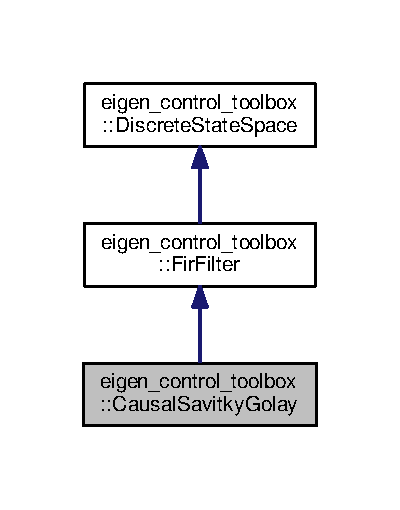
\includegraphics[width=192pt]{classeigen__control__toolbox_1_1_causal_savitky_golay__inherit__graph}
\end{center}
\end{figure}


Collaboration diagram for eigen\+\_\+control\+\_\+toolbox\+:\+:Causal\+Savitky\+Golay\+:
\nopagebreak
\begin{figure}[H]
\begin{center}
\leavevmode
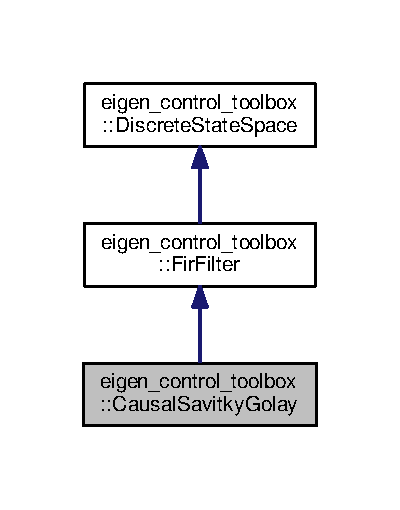
\includegraphics[width=192pt]{classeigen__control__toolbox_1_1_causal_savitky_golay__coll__graph}
\end{center}
\end{figure}
\subsection*{Public Member Functions}
\begin{DoxyCompactItemize}
\item 
\hyperlink{classeigen__control__toolbox_1_1_causal_savitky_golay_aa5b6f458809b32f7a0917e00b30cdb40}{Causal\+Savitky\+Golay} ()
\item 
\hyperlink{classeigen__control__toolbox_1_1_causal_savitky_golay_a3c39b268b53253546ba1a6ab3e1e153d}{Causal\+Savitky\+Golay} (const double \&natural\+\_\+frequency, const double \&sample\+\_\+period, const unsigned int \&polynomial\+\_\+order, const unsigned int \&output\+\_\+size)
\item 
\hyperlink{classeigen__control__toolbox_1_1_causal_savitky_golay_a5b12da27b45af4260d4047708c222965}{Causal\+Savitky\+Golay} (const unsigned int \&window, const double \&sample\+\_\+period, const unsigned int \&polynomial\+\_\+order, const unsigned int \&output\+\_\+size)
\end{DoxyCompactItemize}
\subsection*{Protected Member Functions}
\begin{DoxyCompactItemize}
\item 
void \hyperlink{classeigen__control__toolbox_1_1_causal_savitky_golay_a19c0cd9221aa9239165353c1eb7331e7}{compute\+Coeffs} (const unsigned int \&polynomial\+\_\+order, const unsigned int \&window, const unsigned int \&output\+\_\+size)
\item 
void \hyperlink{classeigen__control__toolbox_1_1_causal_savitky_golay_a4ccf9e0eb474e04b81537f62ac84c96d}{init\+Causal\+Savitky\+Golay} (const double \&natural\+\_\+frequency, const double \&sample\+\_\+period, const unsigned int \&polynomial\+\_\+order, const unsigned int \&output\+\_\+size=1)
\item 
void \hyperlink{classeigen__control__toolbox_1_1_causal_savitky_golay_ae9a466e6bd02cc5cc009d449b6720374}{init\+Causal\+Savitky\+Golay} (const unsigned int \&window, const double \&sample\+\_\+period, const unsigned int \&polynomial\+\_\+order, const unsigned int \&output\+\_\+size=1)
\end{DoxyCompactItemize}
\subsection*{Additional Inherited Members}


\subsection{Detailed Description}


Definition at line 45 of file eigen\+\_\+sg\+\_\+filter.\+h.



\subsection{Constructor \& Destructor Documentation}
\index{eigen\+\_\+control\+\_\+toolbox\+::\+Causal\+Savitky\+Golay@{eigen\+\_\+control\+\_\+toolbox\+::\+Causal\+Savitky\+Golay}!Causal\+Savitky\+Golay@{Causal\+Savitky\+Golay}}
\index{Causal\+Savitky\+Golay@{Causal\+Savitky\+Golay}!eigen\+\_\+control\+\_\+toolbox\+::\+Causal\+Savitky\+Golay@{eigen\+\_\+control\+\_\+toolbox\+::\+Causal\+Savitky\+Golay}}
\subsubsection[{\texorpdfstring{Causal\+Savitky\+Golay()}{CausalSavitkyGolay()}}]{\setlength{\rightskip}{0pt plus 5cm}eigen\+\_\+control\+\_\+toolbox\+::\+Causal\+Savitky\+Golay\+::\+Causal\+Savitky\+Golay (
\begin{DoxyParamCaption}
{}
\end{DoxyParamCaption}
)\hspace{0.3cm}{\ttfamily [inline]}}\hypertarget{classeigen__control__toolbox_1_1_causal_savitky_golay_aa5b6f458809b32f7a0917e00b30cdb40}{}\label{classeigen__control__toolbox_1_1_causal_savitky_golay_aa5b6f458809b32f7a0917e00b30cdb40}


Definition at line 67 of file eigen\+\_\+sg\+\_\+filter.\+h.

\index{eigen\+\_\+control\+\_\+toolbox\+::\+Causal\+Savitky\+Golay@{eigen\+\_\+control\+\_\+toolbox\+::\+Causal\+Savitky\+Golay}!Causal\+Savitky\+Golay@{Causal\+Savitky\+Golay}}
\index{Causal\+Savitky\+Golay@{Causal\+Savitky\+Golay}!eigen\+\_\+control\+\_\+toolbox\+::\+Causal\+Savitky\+Golay@{eigen\+\_\+control\+\_\+toolbox\+::\+Causal\+Savitky\+Golay}}
\subsubsection[{\texorpdfstring{Causal\+Savitky\+Golay(const double \&natural\+\_\+frequency, const double \&sample\+\_\+period, const unsigned int \&polynomial\+\_\+order, const unsigned int \&output\+\_\+size)}{CausalSavitkyGolay(const double &natural_frequency, const double &sample_period, const unsigned int &polynomial_order, const unsigned int &output_size)}}]{\setlength{\rightskip}{0pt plus 5cm}eigen\+\_\+control\+\_\+toolbox\+::\+Causal\+Savitky\+Golay\+::\+Causal\+Savitky\+Golay (
\begin{DoxyParamCaption}
\item[{const double \&}]{natural\+\_\+frequency, }
\item[{const double \&}]{sample\+\_\+period, }
\item[{const unsigned int \&}]{polynomial\+\_\+order, }
\item[{const unsigned int \&}]{output\+\_\+size}
\end{DoxyParamCaption}
)}\hypertarget{classeigen__control__toolbox_1_1_causal_savitky_golay_a3c39b268b53253546ba1a6ab3e1e153d}{}\label{classeigen__control__toolbox_1_1_causal_savitky_golay_a3c39b268b53253546ba1a6ab3e1e153d}


Definition at line 64 of file eigen\+\_\+sg\+\_\+filter.\+cpp.

\index{eigen\+\_\+control\+\_\+toolbox\+::\+Causal\+Savitky\+Golay@{eigen\+\_\+control\+\_\+toolbox\+::\+Causal\+Savitky\+Golay}!Causal\+Savitky\+Golay@{Causal\+Savitky\+Golay}}
\index{Causal\+Savitky\+Golay@{Causal\+Savitky\+Golay}!eigen\+\_\+control\+\_\+toolbox\+::\+Causal\+Savitky\+Golay@{eigen\+\_\+control\+\_\+toolbox\+::\+Causal\+Savitky\+Golay}}
\subsubsection[{\texorpdfstring{Causal\+Savitky\+Golay(const unsigned int \&window, const double \&sample\+\_\+period, const unsigned int \&polynomial\+\_\+order, const unsigned int \&output\+\_\+size)}{CausalSavitkyGolay(const unsigned int &window, const double &sample_period, const unsigned int &polynomial_order, const unsigned int &output_size)}}]{\setlength{\rightskip}{0pt plus 5cm}eigen\+\_\+control\+\_\+toolbox\+::\+Causal\+Savitky\+Golay\+::\+Causal\+Savitky\+Golay (
\begin{DoxyParamCaption}
\item[{const unsigned int \&}]{window, }
\item[{const double \&}]{sample\+\_\+period, }
\item[{const unsigned int \&}]{polynomial\+\_\+order, }
\item[{const unsigned int \&}]{output\+\_\+size}
\end{DoxyParamCaption}
)}\hypertarget{classeigen__control__toolbox_1_1_causal_savitky_golay_a5b12da27b45af4260d4047708c222965}{}\label{classeigen__control__toolbox_1_1_causal_savitky_golay_a5b12da27b45af4260d4047708c222965}


Definition at line 73 of file eigen\+\_\+sg\+\_\+filter.\+cpp.



\subsection{Member Function Documentation}
\index{eigen\+\_\+control\+\_\+toolbox\+::\+Causal\+Savitky\+Golay@{eigen\+\_\+control\+\_\+toolbox\+::\+Causal\+Savitky\+Golay}!compute\+Coeffs@{compute\+Coeffs}}
\index{compute\+Coeffs@{compute\+Coeffs}!eigen\+\_\+control\+\_\+toolbox\+::\+Causal\+Savitky\+Golay@{eigen\+\_\+control\+\_\+toolbox\+::\+Causal\+Savitky\+Golay}}
\subsubsection[{\texorpdfstring{compute\+Coeffs(const unsigned int \&polynomial\+\_\+order, const unsigned int \&window, const unsigned int \&output\+\_\+size)}{computeCoeffs(const unsigned int &polynomial_order, const unsigned int &window, const unsigned int &output_size)}}]{\setlength{\rightskip}{0pt plus 5cm}void eigen\+\_\+control\+\_\+toolbox\+::\+Causal\+Savitky\+Golay\+::compute\+Coeffs (
\begin{DoxyParamCaption}
\item[{const unsigned int \&}]{polynomial\+\_\+order, }
\item[{const unsigned int \&}]{window, }
\item[{const unsigned int \&}]{output\+\_\+size}
\end{DoxyParamCaption}
)\hspace{0.3cm}{\ttfamily [protected]}}\hypertarget{classeigen__control__toolbox_1_1_causal_savitky_golay_a19c0cd9221aa9239165353c1eb7331e7}{}\label{classeigen__control__toolbox_1_1_causal_savitky_golay_a19c0cd9221aa9239165353c1eb7331e7}


Definition at line 103 of file eigen\+\_\+sg\+\_\+filter.\+cpp.

\index{eigen\+\_\+control\+\_\+toolbox\+::\+Causal\+Savitky\+Golay@{eigen\+\_\+control\+\_\+toolbox\+::\+Causal\+Savitky\+Golay}!init\+Causal\+Savitky\+Golay@{init\+Causal\+Savitky\+Golay}}
\index{init\+Causal\+Savitky\+Golay@{init\+Causal\+Savitky\+Golay}!eigen\+\_\+control\+\_\+toolbox\+::\+Causal\+Savitky\+Golay@{eigen\+\_\+control\+\_\+toolbox\+::\+Causal\+Savitky\+Golay}}
\subsubsection[{\texorpdfstring{init\+Causal\+Savitky\+Golay(const double \&natural\+\_\+frequency, const double \&sample\+\_\+period, const unsigned int \&polynomial\+\_\+order, const unsigned int \&output\+\_\+size=1)}{initCausalSavitkyGolay(const double &natural_frequency, const double &sample_period, const unsigned int &polynomial_order, const unsigned int &output_size=1)}}]{\setlength{\rightskip}{0pt plus 5cm}void eigen\+\_\+control\+\_\+toolbox\+::\+Causal\+Savitky\+Golay\+::init\+Causal\+Savitky\+Golay (
\begin{DoxyParamCaption}
\item[{const double \&}]{natural\+\_\+frequency, }
\item[{const double \&}]{sample\+\_\+period, }
\item[{const unsigned int \&}]{polynomial\+\_\+order, }
\item[{const unsigned int \&}]{output\+\_\+size = {\ttfamily 1}}
\end{DoxyParamCaption}
)\hspace{0.3cm}{\ttfamily [protected]}}\hypertarget{classeigen__control__toolbox_1_1_causal_savitky_golay_a4ccf9e0eb474e04b81537f62ac84c96d}{}\label{classeigen__control__toolbox_1_1_causal_savitky_golay_a4ccf9e0eb474e04b81537f62ac84c96d}


Definition at line 78 of file eigen\+\_\+sg\+\_\+filter.\+cpp.

\index{eigen\+\_\+control\+\_\+toolbox\+::\+Causal\+Savitky\+Golay@{eigen\+\_\+control\+\_\+toolbox\+::\+Causal\+Savitky\+Golay}!init\+Causal\+Savitky\+Golay@{init\+Causal\+Savitky\+Golay}}
\index{init\+Causal\+Savitky\+Golay@{init\+Causal\+Savitky\+Golay}!eigen\+\_\+control\+\_\+toolbox\+::\+Causal\+Savitky\+Golay@{eigen\+\_\+control\+\_\+toolbox\+::\+Causal\+Savitky\+Golay}}
\subsubsection[{\texorpdfstring{init\+Causal\+Savitky\+Golay(const unsigned int \&window, const double \&sample\+\_\+period, const unsigned int \&polynomial\+\_\+order, const unsigned int \&output\+\_\+size=1)}{initCausalSavitkyGolay(const unsigned int &window, const double &sample_period, const unsigned int &polynomial_order, const unsigned int &output_size=1)}}]{\setlength{\rightskip}{0pt plus 5cm}void eigen\+\_\+control\+\_\+toolbox\+::\+Causal\+Savitky\+Golay\+::init\+Causal\+Savitky\+Golay (
\begin{DoxyParamCaption}
\item[{const unsigned int \&}]{window, }
\item[{const double \&}]{sample\+\_\+period, }
\item[{const unsigned int \&}]{polynomial\+\_\+order, }
\item[{const unsigned int \&}]{output\+\_\+size = {\ttfamily 1}}
\end{DoxyParamCaption}
)\hspace{0.3cm}{\ttfamily [protected]}}\hypertarget{classeigen__control__toolbox_1_1_causal_savitky_golay_ae9a466e6bd02cc5cc009d449b6720374}{}\label{classeigen__control__toolbox_1_1_causal_savitky_golay_ae9a466e6bd02cc5cc009d449b6720374}


Definition at line 95 of file eigen\+\_\+sg\+\_\+filter.\+cpp.



The documentation for this class was generated from the following files\+:\begin{DoxyCompactItemize}
\item 
include/eigen\+\_\+state\+\_\+space\+\_\+systems/\hyperlink{eigen__sg__filter_8h}{eigen\+\_\+sg\+\_\+filter.\+h}\item 
src/eigen\+\_\+state\+\_\+space\+\_\+systems/\hyperlink{eigen__sg__filter_8cpp}{eigen\+\_\+sg\+\_\+filter.\+cpp}\end{DoxyCompactItemize}

\hypertarget{classeigen__control__toolbox_1_1_controller}{}\section{eigen\+\_\+control\+\_\+toolbox\+:\+:Controller Class Reference}
\label{classeigen__control__toolbox_1_1_controller}\index{eigen\+\_\+control\+\_\+toolbox\+::\+Controller@{eigen\+\_\+control\+\_\+toolbox\+::\+Controller}}


{\ttfamily \#include $<$eigen\+\_\+controllers.\+h$>$}



Inheritance diagram for eigen\+\_\+control\+\_\+toolbox\+:\+:Controller\+:
\nopagebreak
\begin{figure}[H]
\begin{center}
\leavevmode
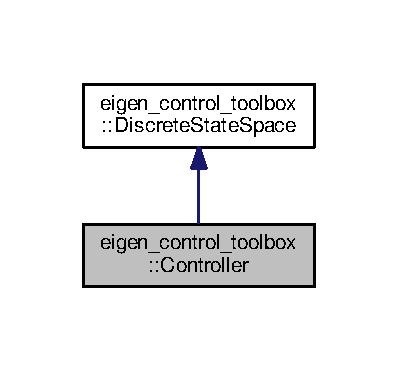
\includegraphics[width=191pt]{classeigen__control__toolbox_1_1_controller__inherit__graph}
\end{center}
\end{figure}


Collaboration diagram for eigen\+\_\+control\+\_\+toolbox\+:\+:Controller\+:
\nopagebreak
\begin{figure}[H]
\begin{center}
\leavevmode
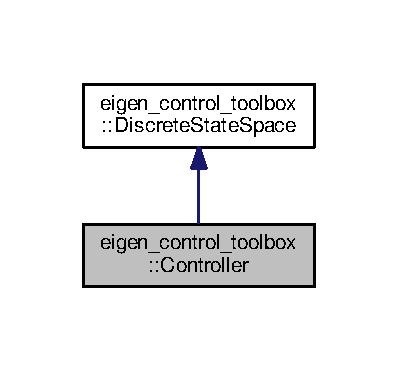
\includegraphics[width=191pt]{classeigen__control__toolbox_1_1_controller__coll__graph}
\end{center}
\end{figure}
\subsection*{Public Member Functions}
\begin{DoxyCompactItemize}
\item 
\hyperlink{classeigen__control__toolbox_1_1_controller_a5e1e2668aa9f0e16940e37e812f90a59}{Controller} ()
\item 
\hyperlink{classeigen__control__toolbox_1_1_controller_a5d0cafdfca0fb15b7ba2a1d343f897ac}{Controller} (const Eigen\+::\+Ref$<$ Eigen\+::\+Matrix\+Xd $>$ A, const Eigen\+::\+Ref$<$ Eigen\+::\+Matrix\+Xd $>$ B, const Eigen\+::\+Ref$<$ Eigen\+::\+Matrix\+Xd $>$ C, const Eigen\+::\+Ref$<$ Eigen\+::\+Matrix\+Xd $>$ D)
\item 
void \hyperlink{classeigen__control__toolbox_1_1_controller_abcf2a726f7b30f9638ec4c263a94849e}{set\+Matrices} (const Eigen\+::\+Ref$<$ Eigen\+::\+Matrix\+Xd $>$ A, const Eigen\+::\+Ref$<$ Eigen\+::\+Matrix\+Xd $>$ B, const Eigen\+::\+Ref$<$ Eigen\+::\+Matrix\+Xd $>$ C, const Eigen\+::\+Ref$<$ Eigen\+::\+Matrix\+Xd $>$ D)
\item 
virtual void \hyperlink{classeigen__control__toolbox_1_1_controller_a63728f95d5d4ab2984f3deb402e23c1f}{set\+Anti\+Windup\+Matrix} (const Eigen\+::\+Ref$<$ Eigen\+::\+Matrix\+Xd $>$ D)
\item 
bool \hyperlink{classeigen__control__toolbox_1_1_controller_a8e4ba86e84ed04596442811d99a2cd1d}{import\+Matrices\+From\+Param} (const ros\+::\+Node\+Handle \&nh, const std\+::string \&controller\+\_\+name)
\item 
virtual Eigen\+::\+Vector\+Xd \hyperlink{classeigen__control__toolbox_1_1_controller_a1091bd414788093e7af2fb89f291266a}{update} (const Eigen\+::\+Ref$<$ Eigen\+::\+Vector\+Xd $>$ input)
\item 
void \hyperlink{classeigen__control__toolbox_1_1_controller_a42c4e78a4a1b012daeaacd437e2d728e}{antiwindup} (const Eigen\+::\+Ref$<$ Eigen\+::\+Vector\+Xd $>$ saturated\+\_\+output, Eigen\+::\+Ref$<$ Eigen\+::\+Vector\+Xd $>$ unsaturated\+\_\+output)
\end{DoxyCompactItemize}
\subsection*{Protected Attributes}
\begin{DoxyCompactItemize}
\item 
Eigen\+::\+Matrix\+Xd \hyperlink{classeigen__control__toolbox_1_1_controller_a02cc421090f12505dd3f7025ff2dd134}{m\+\_\+\+Baw}
\end{DoxyCompactItemize}
\subsection*{Additional Inherited Members}


\subsection{Detailed Description}


Definition at line 8 of file eigen\+\_\+controllers.\+h.



\subsection{Constructor \& Destructor Documentation}
\index{eigen\+\_\+control\+\_\+toolbox\+::\+Controller@{eigen\+\_\+control\+\_\+toolbox\+::\+Controller}!Controller@{Controller}}
\index{Controller@{Controller}!eigen\+\_\+control\+\_\+toolbox\+::\+Controller@{eigen\+\_\+control\+\_\+toolbox\+::\+Controller}}
\subsubsection[{\texorpdfstring{Controller()}{Controller()}}]{\setlength{\rightskip}{0pt plus 5cm}eigen\+\_\+control\+\_\+toolbox\+::\+Controller\+::\+Controller (
\begin{DoxyParamCaption}
{}
\end{DoxyParamCaption}
)}\hypertarget{classeigen__control__toolbox_1_1_controller_a5e1e2668aa9f0e16940e37e812f90a59}{}\label{classeigen__control__toolbox_1_1_controller_a5e1e2668aa9f0e16940e37e812f90a59}


Definition at line 19 of file eigen\+\_\+controllers.\+cpp.

\index{eigen\+\_\+control\+\_\+toolbox\+::\+Controller@{eigen\+\_\+control\+\_\+toolbox\+::\+Controller}!Controller@{Controller}}
\index{Controller@{Controller}!eigen\+\_\+control\+\_\+toolbox\+::\+Controller@{eigen\+\_\+control\+\_\+toolbox\+::\+Controller}}
\subsubsection[{\texorpdfstring{Controller(const Eigen\+::\+Ref$<$ Eigen\+::\+Matrix\+Xd $>$ A, const Eigen\+::\+Ref$<$ Eigen\+::\+Matrix\+Xd $>$ B, const Eigen\+::\+Ref$<$ Eigen\+::\+Matrix\+Xd $>$ C, const Eigen\+::\+Ref$<$ Eigen\+::\+Matrix\+Xd $>$ D)}{Controller(const Eigen::Ref< Eigen::MatrixXd > A, const Eigen::Ref< Eigen::MatrixXd > B, const Eigen::Ref< Eigen::MatrixXd > C, const Eigen::Ref< Eigen::MatrixXd > D)}}]{\setlength{\rightskip}{0pt plus 5cm}eigen\+\_\+control\+\_\+toolbox\+::\+Controller\+::\+Controller (
\begin{DoxyParamCaption}
\item[{const Eigen\+::\+Ref$<$ Eigen\+::\+Matrix\+Xd $>$}]{A, }
\item[{const Eigen\+::\+Ref$<$ Eigen\+::\+Matrix\+Xd $>$}]{B, }
\item[{const Eigen\+::\+Ref$<$ Eigen\+::\+Matrix\+Xd $>$}]{C, }
\item[{const Eigen\+::\+Ref$<$ Eigen\+::\+Matrix\+Xd $>$}]{D}
\end{DoxyParamCaption}
)}\hypertarget{classeigen__control__toolbox_1_1_controller_a5d0cafdfca0fb15b7ba2a1d343f897ac}{}\label{classeigen__control__toolbox_1_1_controller_a5d0cafdfca0fb15b7ba2a1d343f897ac}


Definition at line 6 of file eigen\+\_\+controllers.\+cpp.



\subsection{Member Function Documentation}
\index{eigen\+\_\+control\+\_\+toolbox\+::\+Controller@{eigen\+\_\+control\+\_\+toolbox\+::\+Controller}!antiwindup@{antiwindup}}
\index{antiwindup@{antiwindup}!eigen\+\_\+control\+\_\+toolbox\+::\+Controller@{eigen\+\_\+control\+\_\+toolbox\+::\+Controller}}
\subsubsection[{\texorpdfstring{antiwindup(const Eigen\+::\+Ref$<$ Eigen\+::\+Vector\+Xd $>$ saturated\+\_\+output, Eigen\+::\+Ref$<$ Eigen\+::\+Vector\+Xd $>$ unsaturated\+\_\+output)}{antiwindup(const Eigen::Ref< Eigen::VectorXd > saturated_output, Eigen::Ref< Eigen::VectorXd > unsaturated_output)}}]{\setlength{\rightskip}{0pt plus 5cm}void eigen\+\_\+control\+\_\+toolbox\+::\+Controller\+::antiwindup (
\begin{DoxyParamCaption}
\item[{const Eigen\+::\+Ref$<$ Eigen\+::\+Vector\+Xd $>$}]{saturated\+\_\+output, }
\item[{Eigen\+::\+Ref$<$ Eigen\+::\+Vector\+Xd $>$}]{unsaturated\+\_\+output}
\end{DoxyParamCaption}
)}\hypertarget{classeigen__control__toolbox_1_1_controller_a42c4e78a4a1b012daeaacd437e2d728e}{}\label{classeigen__control__toolbox_1_1_controller_a42c4e78a4a1b012daeaacd437e2d728e}


Definition at line 80 of file eigen\+\_\+controllers.\+cpp.

\index{eigen\+\_\+control\+\_\+toolbox\+::\+Controller@{eigen\+\_\+control\+\_\+toolbox\+::\+Controller}!import\+Matrices\+From\+Param@{import\+Matrices\+From\+Param}}
\index{import\+Matrices\+From\+Param@{import\+Matrices\+From\+Param}!eigen\+\_\+control\+\_\+toolbox\+::\+Controller@{eigen\+\_\+control\+\_\+toolbox\+::\+Controller}}
\subsubsection[{\texorpdfstring{import\+Matrices\+From\+Param(const ros\+::\+Node\+Handle \&nh, const std\+::string \&controller\+\_\+name)}{importMatricesFromParam(const ros::NodeHandle &nh, const std::string &controller_name)}}]{\setlength{\rightskip}{0pt plus 5cm}bool eigen\+\_\+control\+\_\+toolbox\+::\+Controller\+::import\+Matrices\+From\+Param (
\begin{DoxyParamCaption}
\item[{const ros\+::\+Node\+Handle \&}]{nh, }
\item[{const std\+::string \&}]{controller\+\_\+name}
\end{DoxyParamCaption}
)}\hypertarget{classeigen__control__toolbox_1_1_controller_a8e4ba86e84ed04596442811d99a2cd1d}{}\label{classeigen__control__toolbox_1_1_controller_a8e4ba86e84ed04596442811d99a2cd1d}


Definition at line 34 of file eigen\+\_\+controllers.\+cpp.

\index{eigen\+\_\+control\+\_\+toolbox\+::\+Controller@{eigen\+\_\+control\+\_\+toolbox\+::\+Controller}!set\+Anti\+Windup\+Matrix@{set\+Anti\+Windup\+Matrix}}
\index{set\+Anti\+Windup\+Matrix@{set\+Anti\+Windup\+Matrix}!eigen\+\_\+control\+\_\+toolbox\+::\+Controller@{eigen\+\_\+control\+\_\+toolbox\+::\+Controller}}
\subsubsection[{\texorpdfstring{set\+Anti\+Windup\+Matrix(const Eigen\+::\+Ref$<$ Eigen\+::\+Matrix\+Xd $>$ D)}{setAntiWindupMatrix(const Eigen::Ref< Eigen::MatrixXd > D)}}]{\setlength{\rightskip}{0pt plus 5cm}void eigen\+\_\+control\+\_\+toolbox\+::\+Controller\+::set\+Anti\+Windup\+Matrix (
\begin{DoxyParamCaption}
\item[{const Eigen\+::\+Ref$<$ Eigen\+::\+Matrix\+Xd $>$}]{D}
\end{DoxyParamCaption}
)\hspace{0.3cm}{\ttfamily [virtual]}}\hypertarget{classeigen__control__toolbox_1_1_controller_a63728f95d5d4ab2984f3deb402e23c1f}{}\label{classeigen__control__toolbox_1_1_controller_a63728f95d5d4ab2984f3deb402e23c1f}


Definition at line 26 of file eigen\+\_\+controllers.\+cpp.

\index{eigen\+\_\+control\+\_\+toolbox\+::\+Controller@{eigen\+\_\+control\+\_\+toolbox\+::\+Controller}!set\+Matrices@{set\+Matrices}}
\index{set\+Matrices@{set\+Matrices}!eigen\+\_\+control\+\_\+toolbox\+::\+Controller@{eigen\+\_\+control\+\_\+toolbox\+::\+Controller}}
\subsubsection[{\texorpdfstring{set\+Matrices(const Eigen\+::\+Ref$<$ Eigen\+::\+Matrix\+Xd $>$ A, const Eigen\+::\+Ref$<$ Eigen\+::\+Matrix\+Xd $>$ B, const Eigen\+::\+Ref$<$ Eigen\+::\+Matrix\+Xd $>$ C, const Eigen\+::\+Ref$<$ Eigen\+::\+Matrix\+Xd $>$ D)}{setMatrices(const Eigen::Ref< Eigen::MatrixXd > A, const Eigen::Ref< Eigen::MatrixXd > B, const Eigen::Ref< Eigen::MatrixXd > C, const Eigen::Ref< Eigen::MatrixXd > D)}}]{\setlength{\rightskip}{0pt plus 5cm}void eigen\+\_\+control\+\_\+toolbox\+::\+Controller\+::set\+Matrices (
\begin{DoxyParamCaption}
\item[{const Eigen\+::\+Ref$<$ Eigen\+::\+Matrix\+Xd $>$}]{A, }
\item[{const Eigen\+::\+Ref$<$ Eigen\+::\+Matrix\+Xd $>$}]{B, }
\item[{const Eigen\+::\+Ref$<$ Eigen\+::\+Matrix\+Xd $>$}]{C, }
\item[{const Eigen\+::\+Ref$<$ Eigen\+::\+Matrix\+Xd $>$}]{D}
\end{DoxyParamCaption}
)\hspace{0.3cm}{\ttfamily [virtual]}}\hypertarget{classeigen__control__toolbox_1_1_controller_abcf2a726f7b30f9638ec4c263a94849e}{}\label{classeigen__control__toolbox_1_1_controller_abcf2a726f7b30f9638ec4c263a94849e}


Reimplemented from \hyperlink{classeigen__control__toolbox_1_1_discrete_state_space_a283b4074b1814d3bbc8c9cc8abb58bbe}{eigen\+\_\+control\+\_\+toolbox\+::\+Discrete\+State\+Space}.



Definition at line 11 of file eigen\+\_\+controllers.\+cpp.

\index{eigen\+\_\+control\+\_\+toolbox\+::\+Controller@{eigen\+\_\+control\+\_\+toolbox\+::\+Controller}!update@{update}}
\index{update@{update}!eigen\+\_\+control\+\_\+toolbox\+::\+Controller@{eigen\+\_\+control\+\_\+toolbox\+::\+Controller}}
\subsubsection[{\texorpdfstring{update(const Eigen\+::\+Ref$<$ Eigen\+::\+Vector\+Xd $>$ input)}{update(const Eigen::Ref< Eigen::VectorXd > input)}}]{\setlength{\rightskip}{0pt plus 5cm}Eigen\+::\+Vector\+Xd eigen\+\_\+control\+\_\+toolbox\+::\+Controller\+::update (
\begin{DoxyParamCaption}
\item[{const Eigen\+::\+Ref$<$ Eigen\+::\+Vector\+Xd $>$}]{input}
\end{DoxyParamCaption}
)\hspace{0.3cm}{\ttfamily [virtual]}}\hypertarget{classeigen__control__toolbox_1_1_controller_a1091bd414788093e7af2fb89f291266a}{}\label{classeigen__control__toolbox_1_1_controller_a1091bd414788093e7af2fb89f291266a}


Reimplemented from \hyperlink{classeigen__control__toolbox_1_1_discrete_state_space_ae58e06527268253cea809554a528fdfe}{eigen\+\_\+control\+\_\+toolbox\+::\+Discrete\+State\+Space}.



Definition at line 75 of file eigen\+\_\+controllers.\+cpp.



\subsection{Member Data Documentation}
\index{eigen\+\_\+control\+\_\+toolbox\+::\+Controller@{eigen\+\_\+control\+\_\+toolbox\+::\+Controller}!m\+\_\+\+Baw@{m\+\_\+\+Baw}}
\index{m\+\_\+\+Baw@{m\+\_\+\+Baw}!eigen\+\_\+control\+\_\+toolbox\+::\+Controller@{eigen\+\_\+control\+\_\+toolbox\+::\+Controller}}
\subsubsection[{\texorpdfstring{m\+\_\+\+Baw}{m_Baw}}]{\setlength{\rightskip}{0pt plus 5cm}Eigen\+::\+Matrix\+Xd eigen\+\_\+control\+\_\+toolbox\+::\+Controller\+::m\+\_\+\+Baw\hspace{0.3cm}{\ttfamily [protected]}}\hypertarget{classeigen__control__toolbox_1_1_controller_a02cc421090f12505dd3f7025ff2dd134}{}\label{classeigen__control__toolbox_1_1_controller_a02cc421090f12505dd3f7025ff2dd134}


Definition at line 11 of file eigen\+\_\+controllers.\+h.



The documentation for this class was generated from the following files\+:\begin{DoxyCompactItemize}
\item 
include/eigen\+\_\+state\+\_\+space\+\_\+systems/\hyperlink{eigen__controllers_8h}{eigen\+\_\+controllers.\+h}\item 
src/eigen\+\_\+state\+\_\+space\+\_\+systems/\hyperlink{eigen__controllers_8cpp}{eigen\+\_\+controllers.\+cpp}\end{DoxyCompactItemize}

\hypertarget{classeigen__control__toolbox_1_1_discrete_state_space}{}\section{eigen\+\_\+control\+\_\+toolbox\+:\+:Discrete\+State\+Space Class Reference}
\label{classeigen__control__toolbox_1_1_discrete_state_space}\index{eigen\+\_\+control\+\_\+toolbox\+::\+Discrete\+State\+Space@{eigen\+\_\+control\+\_\+toolbox\+::\+Discrete\+State\+Space}}


{\ttfamily \#include $<$eigen\+\_\+state\+\_\+space\+\_\+systems.\+h$>$}



Inheritance diagram for eigen\+\_\+control\+\_\+toolbox\+:\+:Discrete\+State\+Space\+:
\nopagebreak
\begin{figure}[H]
\begin{center}
\leavevmode
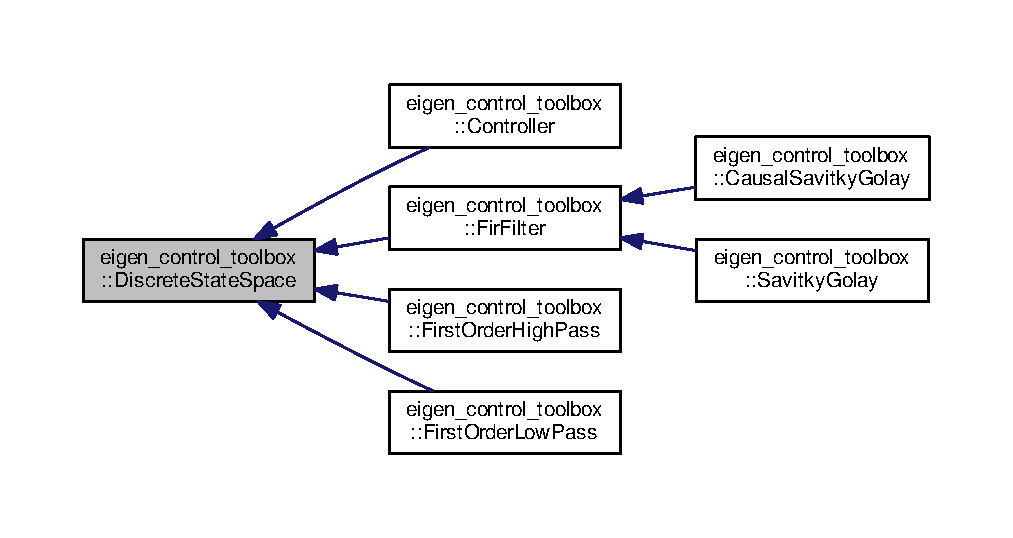
\includegraphics[width=350pt]{classeigen__control__toolbox_1_1_discrete_state_space__inherit__graph}
\end{center}
\end{figure}
\subsection*{Public Member Functions}
\begin{DoxyCompactItemize}
\item 
\hyperlink{classeigen__control__toolbox_1_1_discrete_state_space_a205064d804989e5d6d00af4d54386b66}{Discrete\+State\+Space} ()
\item 
\hyperlink{classeigen__control__toolbox_1_1_discrete_state_space_a67e56fac91f99ded7bd5f252a4a4c241}{Discrete\+State\+Space} (const Eigen\+::\+Ref$<$ Eigen\+::\+Matrix\+Xd $>$ A, const Eigen\+::\+Ref$<$ Eigen\+::\+Matrix\+Xd $>$ B, const Eigen\+::\+Ref$<$ Eigen\+::\+Matrix\+Xd $>$ C, const Eigen\+::\+Ref$<$ Eigen\+::\+Matrix\+Xd $>$ D)
\item 
bool \hyperlink{classeigen__control__toolbox_1_1_discrete_state_space_aa6c1fd6786d35dc12b2c4add8799b9e3}{import\+Matrices\+From\+Param} (const ros\+::\+Node\+Handle \&nh, const std\+::\+\_\+\+\_\+cxx11\+::string \&name)
\item 
Eigen\+::\+Matrix\+Xd \hyperlink{classeigen__control__toolbox_1_1_discrete_state_space_af98f9769460769dd5e40328769deb0d1}{get\+A\+Matrix} ()
\item 
Eigen\+::\+Matrix\+Xd \hyperlink{classeigen__control__toolbox_1_1_discrete_state_space_a0031698ccb43b578ebf7357d8ddeef9d}{get\+B\+Matrix} ()
\item 
Eigen\+::\+Matrix\+Xd \hyperlink{classeigen__control__toolbox_1_1_discrete_state_space_a302df76daf30ffa0f3740292155a67d9}{get\+C\+Matrix} ()
\item 
Eigen\+::\+Matrix\+Xd \hyperlink{classeigen__control__toolbox_1_1_discrete_state_space_a760410cc7727d002aa5fa09493e73d84}{get\+D\+Matrix} ()
\item 
Eigen\+::\+Vector\+Xd \hyperlink{classeigen__control__toolbox_1_1_discrete_state_space_a5f558aad3c0df6f779ee9f29a2f0f5c7}{get\+Output} ()
\item 
Eigen\+::\+Vector\+Xd \hyperlink{classeigen__control__toolbox_1_1_discrete_state_space_a48aa4afa8467bc719cfec7b350e555a5}{get\+State} ()
\item 
unsigned int \hyperlink{classeigen__control__toolbox_1_1_discrete_state_space_af2cf915334b74c04f3eae9405c34d0a9}{get\+Order} ()
\item 
unsigned int \hyperlink{classeigen__control__toolbox_1_1_discrete_state_space_a449fa9b037f7de46c84eb9a3248074c8}{get\+Number\+Of\+Inputs} ()
\item 
unsigned int \hyperlink{classeigen__control__toolbox_1_1_discrete_state_space_a43ef1ca41a2fff19826b1d865c35e368}{get\+Number\+Of\+Outputs} ()
\item 
void \hyperlink{classeigen__control__toolbox_1_1_discrete_state_space_a822ee5d7d4bebbdf991f95dee1092775}{set\+State} (const Eigen\+::\+Ref$<$ Eigen\+::\+Vector\+Xd $>$ state)
\item 
void \hyperlink{classeigen__control__toolbox_1_1_discrete_state_space_af8e7d1aa7a8315d116e7a5dae24fcab1}{set\+Sampling\+Period} (const double \&sampling\+\_\+period)
\item 
double \hyperlink{classeigen__control__toolbox_1_1_discrete_state_space_a1c8a67c5d72db57da35d4482265ef59b}{get\+Sampling\+Period} ()
\item 
virtual void \hyperlink{classeigen__control__toolbox_1_1_discrete_state_space_a5965984530e7b3b915883d9a287e2d14}{set\+State\+From\+IO} (const Eigen\+::\+Ref$<$ Eigen\+::\+Vector\+Xd $>$ past\+\_\+inputs, const Eigen\+::\+Ref$<$ Eigen\+::\+Vector\+Xd $>$ past\+\_\+outputs)
\item 
void \hyperlink{classeigen__control__toolbox_1_1_discrete_state_space_af3f95bc7110bc5b9aa920afbe81a54b2}{set\+State\+From\+Last\+IO} (const Eigen\+::\+Ref$<$ Eigen\+::\+Vector\+Xd $>$ inputs, const Eigen\+::\+Ref$<$ Eigen\+::\+Vector\+Xd $>$ outputs)
\item 
virtual Eigen\+::\+Vector\+Xd \hyperlink{classeigen__control__toolbox_1_1_discrete_state_space_ae58e06527268253cea809554a528fdfe}{update} (const Eigen\+::\+Ref$<$ Eigen\+::\+Vector\+Xd $>$ input)
\item 
virtual double \hyperlink{classeigen__control__toolbox_1_1_discrete_state_space_afff4d00311c12501f8a72d1312d8c5ef}{update} (const double \&input)
\end{DoxyCompactItemize}
\subsection*{Protected Member Functions}
\begin{DoxyCompactItemize}
\item 
virtual void \hyperlink{classeigen__control__toolbox_1_1_discrete_state_space_a283b4074b1814d3bbc8c9cc8abb58bbe}{set\+Matrices} (const Eigen\+::\+Ref$<$ Eigen\+::\+Matrix\+Xd $>$ A, const Eigen\+::\+Ref$<$ Eigen\+::\+Matrix\+Xd $>$ B, const Eigen\+::\+Ref$<$ Eigen\+::\+Matrix\+Xd $>$ C, const Eigen\+::\+Ref$<$ Eigen\+::\+Matrix\+Xd $>$ D)
\end{DoxyCompactItemize}
\subsection*{Protected Attributes}
\begin{DoxyCompactItemize}
\item 
unsigned int \hyperlink{classeigen__control__toolbox_1_1_discrete_state_space_af226df79174f11922017e18ebb45e89b}{m\+\_\+order}
\item 
unsigned int \hyperlink{classeigen__control__toolbox_1_1_discrete_state_space_a28d1ee83fe68a634516e4bcf53990954}{m\+\_\+nin}
\item 
unsigned int \hyperlink{classeigen__control__toolbox_1_1_discrete_state_space_a709da4473200de4bfff97932bf3efd64}{m\+\_\+nout}
\item 
double \hyperlink{classeigen__control__toolbox_1_1_discrete_state_space_a2762ef0b3292b24ebef3b7ba24501cc4}{m\+\_\+sampling\+\_\+period}
\item 
Eigen\+::\+Vector\+Xd \hyperlink{classeigen__control__toolbox_1_1_discrete_state_space_afd14e426784cd7a76ee6e5258e3602b0}{m\+\_\+state}
\item 
Eigen\+::\+Vector\+Xd \hyperlink{classeigen__control__toolbox_1_1_discrete_state_space_ae78eb5b248f0780f0c417eafa2b85a6b}{m\+\_\+output}
\item 
Eigen\+::\+Matrix\+Xd \hyperlink{classeigen__control__toolbox_1_1_discrete_state_space_a3ced02e4b0aa4d87b9739f452aa208b8}{m\+\_\+A}
\item 
Eigen\+::\+Matrix\+Xd \hyperlink{classeigen__control__toolbox_1_1_discrete_state_space_a070fcc68df2ae0b39af3d308a1c5011f}{m\+\_\+B}
\item 
Eigen\+::\+Matrix\+Xd \hyperlink{classeigen__control__toolbox_1_1_discrete_state_space_ac3a719d7d124200b9d67b9df525024bb}{m\+\_\+C}
\item 
Eigen\+::\+Matrix\+Xd \hyperlink{classeigen__control__toolbox_1_1_discrete_state_space_a1f3638e25fd3c1fb9187426133a1a6e3}{m\+\_\+D}
\end{DoxyCompactItemize}


\subsection{Detailed Description}


Definition at line 13 of file eigen\+\_\+state\+\_\+space\+\_\+systems.\+h.



\subsection{Constructor \& Destructor Documentation}
\index{eigen\+\_\+control\+\_\+toolbox\+::\+Discrete\+State\+Space@{eigen\+\_\+control\+\_\+toolbox\+::\+Discrete\+State\+Space}!Discrete\+State\+Space@{Discrete\+State\+Space}}
\index{Discrete\+State\+Space@{Discrete\+State\+Space}!eigen\+\_\+control\+\_\+toolbox\+::\+Discrete\+State\+Space@{eigen\+\_\+control\+\_\+toolbox\+::\+Discrete\+State\+Space}}
\subsubsection[{\texorpdfstring{Discrete\+State\+Space()}{DiscreteStateSpace()}}]{\setlength{\rightskip}{0pt plus 5cm}eigen\+\_\+control\+\_\+toolbox\+::\+Discrete\+State\+Space\+::\+Discrete\+State\+Space (
\begin{DoxyParamCaption}
{}
\end{DoxyParamCaption}
)\hspace{0.3cm}{\ttfamily [inline]}}\hypertarget{classeigen__control__toolbox_1_1_discrete_state_space_a205064d804989e5d6d00af4d54386b66}{}\label{classeigen__control__toolbox_1_1_discrete_state_space_a205064d804989e5d6d00af4d54386b66}


Definition at line 35 of file eigen\+\_\+state\+\_\+space\+\_\+systems.\+h.

\index{eigen\+\_\+control\+\_\+toolbox\+::\+Discrete\+State\+Space@{eigen\+\_\+control\+\_\+toolbox\+::\+Discrete\+State\+Space}!Discrete\+State\+Space@{Discrete\+State\+Space}}
\index{Discrete\+State\+Space@{Discrete\+State\+Space}!eigen\+\_\+control\+\_\+toolbox\+::\+Discrete\+State\+Space@{eigen\+\_\+control\+\_\+toolbox\+::\+Discrete\+State\+Space}}
\subsubsection[{\texorpdfstring{Discrete\+State\+Space(const Eigen\+::\+Ref$<$ Eigen\+::\+Matrix\+Xd $>$ A, const Eigen\+::\+Ref$<$ Eigen\+::\+Matrix\+Xd $>$ B, const Eigen\+::\+Ref$<$ Eigen\+::\+Matrix\+Xd $>$ C, const Eigen\+::\+Ref$<$ Eigen\+::\+Matrix\+Xd $>$ D)}{DiscreteStateSpace(const Eigen::Ref< Eigen::MatrixXd > A, const Eigen::Ref< Eigen::MatrixXd > B, const Eigen::Ref< Eigen::MatrixXd > C, const Eigen::Ref< Eigen::MatrixXd > D)}}]{\setlength{\rightskip}{0pt plus 5cm}eigen\+\_\+control\+\_\+toolbox\+::\+Discrete\+State\+Space\+::\+Discrete\+State\+Space (
\begin{DoxyParamCaption}
\item[{const Eigen\+::\+Ref$<$ Eigen\+::\+Matrix\+Xd $>$}]{A, }
\item[{const Eigen\+::\+Ref$<$ Eigen\+::\+Matrix\+Xd $>$}]{B, }
\item[{const Eigen\+::\+Ref$<$ Eigen\+::\+Matrix\+Xd $>$}]{C, }
\item[{const Eigen\+::\+Ref$<$ Eigen\+::\+Matrix\+Xd $>$}]{D}
\end{DoxyParamCaption}
)}\hypertarget{classeigen__control__toolbox_1_1_discrete_state_space_a67e56fac91f99ded7bd5f252a4a4c241}{}\label{classeigen__control__toolbox_1_1_discrete_state_space_a67e56fac91f99ded7bd5f252a4a4c241}


Definition at line 9 of file eigen\+\_\+state\+\_\+space\+\_\+systems.\+cpp.



\subsection{Member Function Documentation}
\index{eigen\+\_\+control\+\_\+toolbox\+::\+Discrete\+State\+Space@{eigen\+\_\+control\+\_\+toolbox\+::\+Discrete\+State\+Space}!get\+A\+Matrix@{get\+A\+Matrix}}
\index{get\+A\+Matrix@{get\+A\+Matrix}!eigen\+\_\+control\+\_\+toolbox\+::\+Discrete\+State\+Space@{eigen\+\_\+control\+\_\+toolbox\+::\+Discrete\+State\+Space}}
\subsubsection[{\texorpdfstring{get\+A\+Matrix()}{getAMatrix()}}]{\setlength{\rightskip}{0pt plus 5cm}Eigen\+::\+Matrix\+Xd eigen\+\_\+control\+\_\+toolbox\+::\+Discrete\+State\+Space\+::get\+A\+Matrix (
\begin{DoxyParamCaption}
{}
\end{DoxyParamCaption}
)\hspace{0.3cm}{\ttfamily [inline]}}\hypertarget{classeigen__control__toolbox_1_1_discrete_state_space_af98f9769460769dd5e40328769deb0d1}{}\label{classeigen__control__toolbox_1_1_discrete_state_space_af98f9769460769dd5e40328769deb0d1}


Definition at line 43 of file eigen\+\_\+state\+\_\+space\+\_\+systems.\+h.

\index{eigen\+\_\+control\+\_\+toolbox\+::\+Discrete\+State\+Space@{eigen\+\_\+control\+\_\+toolbox\+::\+Discrete\+State\+Space}!get\+B\+Matrix@{get\+B\+Matrix}}
\index{get\+B\+Matrix@{get\+B\+Matrix}!eigen\+\_\+control\+\_\+toolbox\+::\+Discrete\+State\+Space@{eigen\+\_\+control\+\_\+toolbox\+::\+Discrete\+State\+Space}}
\subsubsection[{\texorpdfstring{get\+B\+Matrix()}{getBMatrix()}}]{\setlength{\rightskip}{0pt plus 5cm}Eigen\+::\+Matrix\+Xd eigen\+\_\+control\+\_\+toolbox\+::\+Discrete\+State\+Space\+::get\+B\+Matrix (
\begin{DoxyParamCaption}
{}
\end{DoxyParamCaption}
)\hspace{0.3cm}{\ttfamily [inline]}}\hypertarget{classeigen__control__toolbox_1_1_discrete_state_space_a0031698ccb43b578ebf7357d8ddeef9d}{}\label{classeigen__control__toolbox_1_1_discrete_state_space_a0031698ccb43b578ebf7357d8ddeef9d}


Definition at line 44 of file eigen\+\_\+state\+\_\+space\+\_\+systems.\+h.

\index{eigen\+\_\+control\+\_\+toolbox\+::\+Discrete\+State\+Space@{eigen\+\_\+control\+\_\+toolbox\+::\+Discrete\+State\+Space}!get\+C\+Matrix@{get\+C\+Matrix}}
\index{get\+C\+Matrix@{get\+C\+Matrix}!eigen\+\_\+control\+\_\+toolbox\+::\+Discrete\+State\+Space@{eigen\+\_\+control\+\_\+toolbox\+::\+Discrete\+State\+Space}}
\subsubsection[{\texorpdfstring{get\+C\+Matrix()}{getCMatrix()}}]{\setlength{\rightskip}{0pt plus 5cm}Eigen\+::\+Matrix\+Xd eigen\+\_\+control\+\_\+toolbox\+::\+Discrete\+State\+Space\+::get\+C\+Matrix (
\begin{DoxyParamCaption}
{}
\end{DoxyParamCaption}
)\hspace{0.3cm}{\ttfamily [inline]}}\hypertarget{classeigen__control__toolbox_1_1_discrete_state_space_a302df76daf30ffa0f3740292155a67d9}{}\label{classeigen__control__toolbox_1_1_discrete_state_space_a302df76daf30ffa0f3740292155a67d9}


Definition at line 45 of file eigen\+\_\+state\+\_\+space\+\_\+systems.\+h.

\index{eigen\+\_\+control\+\_\+toolbox\+::\+Discrete\+State\+Space@{eigen\+\_\+control\+\_\+toolbox\+::\+Discrete\+State\+Space}!get\+D\+Matrix@{get\+D\+Matrix}}
\index{get\+D\+Matrix@{get\+D\+Matrix}!eigen\+\_\+control\+\_\+toolbox\+::\+Discrete\+State\+Space@{eigen\+\_\+control\+\_\+toolbox\+::\+Discrete\+State\+Space}}
\subsubsection[{\texorpdfstring{get\+D\+Matrix()}{getDMatrix()}}]{\setlength{\rightskip}{0pt plus 5cm}Eigen\+::\+Matrix\+Xd eigen\+\_\+control\+\_\+toolbox\+::\+Discrete\+State\+Space\+::get\+D\+Matrix (
\begin{DoxyParamCaption}
{}
\end{DoxyParamCaption}
)\hspace{0.3cm}{\ttfamily [inline]}}\hypertarget{classeigen__control__toolbox_1_1_discrete_state_space_a760410cc7727d002aa5fa09493e73d84}{}\label{classeigen__control__toolbox_1_1_discrete_state_space_a760410cc7727d002aa5fa09493e73d84}


Definition at line 46 of file eigen\+\_\+state\+\_\+space\+\_\+systems.\+h.

\index{eigen\+\_\+control\+\_\+toolbox\+::\+Discrete\+State\+Space@{eigen\+\_\+control\+\_\+toolbox\+::\+Discrete\+State\+Space}!get\+Number\+Of\+Inputs@{get\+Number\+Of\+Inputs}}
\index{get\+Number\+Of\+Inputs@{get\+Number\+Of\+Inputs}!eigen\+\_\+control\+\_\+toolbox\+::\+Discrete\+State\+Space@{eigen\+\_\+control\+\_\+toolbox\+::\+Discrete\+State\+Space}}
\subsubsection[{\texorpdfstring{get\+Number\+Of\+Inputs()}{getNumberOfInputs()}}]{\setlength{\rightskip}{0pt plus 5cm}unsigned int eigen\+\_\+control\+\_\+toolbox\+::\+Discrete\+State\+Space\+::get\+Number\+Of\+Inputs (
\begin{DoxyParamCaption}
{}
\end{DoxyParamCaption}
)\hspace{0.3cm}{\ttfamily [inline]}}\hypertarget{classeigen__control__toolbox_1_1_discrete_state_space_a449fa9b037f7de46c84eb9a3248074c8}{}\label{classeigen__control__toolbox_1_1_discrete_state_space_a449fa9b037f7de46c84eb9a3248074c8}


Definition at line 50 of file eigen\+\_\+state\+\_\+space\+\_\+systems.\+h.

\index{eigen\+\_\+control\+\_\+toolbox\+::\+Discrete\+State\+Space@{eigen\+\_\+control\+\_\+toolbox\+::\+Discrete\+State\+Space}!get\+Number\+Of\+Outputs@{get\+Number\+Of\+Outputs}}
\index{get\+Number\+Of\+Outputs@{get\+Number\+Of\+Outputs}!eigen\+\_\+control\+\_\+toolbox\+::\+Discrete\+State\+Space@{eigen\+\_\+control\+\_\+toolbox\+::\+Discrete\+State\+Space}}
\subsubsection[{\texorpdfstring{get\+Number\+Of\+Outputs()}{getNumberOfOutputs()}}]{\setlength{\rightskip}{0pt plus 5cm}unsigned int eigen\+\_\+control\+\_\+toolbox\+::\+Discrete\+State\+Space\+::get\+Number\+Of\+Outputs (
\begin{DoxyParamCaption}
{}
\end{DoxyParamCaption}
)\hspace{0.3cm}{\ttfamily [inline]}}\hypertarget{classeigen__control__toolbox_1_1_discrete_state_space_a43ef1ca41a2fff19826b1d865c35e368}{}\label{classeigen__control__toolbox_1_1_discrete_state_space_a43ef1ca41a2fff19826b1d865c35e368}


Definition at line 51 of file eigen\+\_\+state\+\_\+space\+\_\+systems.\+h.

\index{eigen\+\_\+control\+\_\+toolbox\+::\+Discrete\+State\+Space@{eigen\+\_\+control\+\_\+toolbox\+::\+Discrete\+State\+Space}!get\+Order@{get\+Order}}
\index{get\+Order@{get\+Order}!eigen\+\_\+control\+\_\+toolbox\+::\+Discrete\+State\+Space@{eigen\+\_\+control\+\_\+toolbox\+::\+Discrete\+State\+Space}}
\subsubsection[{\texorpdfstring{get\+Order()}{getOrder()}}]{\setlength{\rightskip}{0pt plus 5cm}unsigned int eigen\+\_\+control\+\_\+toolbox\+::\+Discrete\+State\+Space\+::get\+Order (
\begin{DoxyParamCaption}
{}
\end{DoxyParamCaption}
)\hspace{0.3cm}{\ttfamily [inline]}}\hypertarget{classeigen__control__toolbox_1_1_discrete_state_space_af2cf915334b74c04f3eae9405c34d0a9}{}\label{classeigen__control__toolbox_1_1_discrete_state_space_af2cf915334b74c04f3eae9405c34d0a9}


Definition at line 49 of file eigen\+\_\+state\+\_\+space\+\_\+systems.\+h.

\index{eigen\+\_\+control\+\_\+toolbox\+::\+Discrete\+State\+Space@{eigen\+\_\+control\+\_\+toolbox\+::\+Discrete\+State\+Space}!get\+Output@{get\+Output}}
\index{get\+Output@{get\+Output}!eigen\+\_\+control\+\_\+toolbox\+::\+Discrete\+State\+Space@{eigen\+\_\+control\+\_\+toolbox\+::\+Discrete\+State\+Space}}
\subsubsection[{\texorpdfstring{get\+Output()}{getOutput()}}]{\setlength{\rightskip}{0pt plus 5cm}Eigen\+::\+Vector\+Xd eigen\+\_\+control\+\_\+toolbox\+::\+Discrete\+State\+Space\+::get\+Output (
\begin{DoxyParamCaption}
{}
\end{DoxyParamCaption}
)\hspace{0.3cm}{\ttfamily [inline]}}\hypertarget{classeigen__control__toolbox_1_1_discrete_state_space_a5f558aad3c0df6f779ee9f29a2f0f5c7}{}\label{classeigen__control__toolbox_1_1_discrete_state_space_a5f558aad3c0df6f779ee9f29a2f0f5c7}


Definition at line 47 of file eigen\+\_\+state\+\_\+space\+\_\+systems.\+h.

\index{eigen\+\_\+control\+\_\+toolbox\+::\+Discrete\+State\+Space@{eigen\+\_\+control\+\_\+toolbox\+::\+Discrete\+State\+Space}!get\+Sampling\+Period@{get\+Sampling\+Period}}
\index{get\+Sampling\+Period@{get\+Sampling\+Period}!eigen\+\_\+control\+\_\+toolbox\+::\+Discrete\+State\+Space@{eigen\+\_\+control\+\_\+toolbox\+::\+Discrete\+State\+Space}}
\subsubsection[{\texorpdfstring{get\+Sampling\+Period()}{getSamplingPeriod()}}]{\setlength{\rightskip}{0pt plus 5cm}double eigen\+\_\+control\+\_\+toolbox\+::\+Discrete\+State\+Space\+::get\+Sampling\+Period (
\begin{DoxyParamCaption}
{}
\end{DoxyParamCaption}
)\hspace{0.3cm}{\ttfamily [inline]}}\hypertarget{classeigen__control__toolbox_1_1_discrete_state_space_a1c8a67c5d72db57da35d4482265ef59b}{}\label{classeigen__control__toolbox_1_1_discrete_state_space_a1c8a67c5d72db57da35d4482265ef59b}


Definition at line 56 of file eigen\+\_\+state\+\_\+space\+\_\+systems.\+h.

\index{eigen\+\_\+control\+\_\+toolbox\+::\+Discrete\+State\+Space@{eigen\+\_\+control\+\_\+toolbox\+::\+Discrete\+State\+Space}!get\+State@{get\+State}}
\index{get\+State@{get\+State}!eigen\+\_\+control\+\_\+toolbox\+::\+Discrete\+State\+Space@{eigen\+\_\+control\+\_\+toolbox\+::\+Discrete\+State\+Space}}
\subsubsection[{\texorpdfstring{get\+State()}{getState()}}]{\setlength{\rightskip}{0pt plus 5cm}Eigen\+::\+Vector\+Xd eigen\+\_\+control\+\_\+toolbox\+::\+Discrete\+State\+Space\+::get\+State (
\begin{DoxyParamCaption}
{}
\end{DoxyParamCaption}
)\hspace{0.3cm}{\ttfamily [inline]}}\hypertarget{classeigen__control__toolbox_1_1_discrete_state_space_a48aa4afa8467bc719cfec7b350e555a5}{}\label{classeigen__control__toolbox_1_1_discrete_state_space_a48aa4afa8467bc719cfec7b350e555a5}


Definition at line 48 of file eigen\+\_\+state\+\_\+space\+\_\+systems.\+h.

\index{eigen\+\_\+control\+\_\+toolbox\+::\+Discrete\+State\+Space@{eigen\+\_\+control\+\_\+toolbox\+::\+Discrete\+State\+Space}!import\+Matrices\+From\+Param@{import\+Matrices\+From\+Param}}
\index{import\+Matrices\+From\+Param@{import\+Matrices\+From\+Param}!eigen\+\_\+control\+\_\+toolbox\+::\+Discrete\+State\+Space@{eigen\+\_\+control\+\_\+toolbox\+::\+Discrete\+State\+Space}}
\subsubsection[{\texorpdfstring{import\+Matrices\+From\+Param(const ros\+::\+Node\+Handle \&nh, const std\+::\+\_\+\+\_\+cxx11\+::string \&name)}{importMatricesFromParam(const ros::NodeHandle &nh, const std::__cxx11::string &name)}}]{\setlength{\rightskip}{0pt plus 5cm}bool eigen\+\_\+control\+\_\+toolbox\+::\+Discrete\+State\+Space\+::import\+Matrices\+From\+Param (
\begin{DoxyParamCaption}
\item[{const ros\+::\+Node\+Handle \&}]{nh, }
\item[{const std\+::\+\_\+\+\_\+cxx11\+::string \&}]{name}
\end{DoxyParamCaption}
)}\hypertarget{classeigen__control__toolbox_1_1_discrete_state_space_aa6c1fd6786d35dc12b2c4add8799b9e3}{}\label{classeigen__control__toolbox_1_1_discrete_state_space_aa6c1fd6786d35dc12b2c4add8799b9e3}


Definition at line 121 of file eigen\+\_\+state\+\_\+space\+\_\+systems.\+cpp.

\index{eigen\+\_\+control\+\_\+toolbox\+::\+Discrete\+State\+Space@{eigen\+\_\+control\+\_\+toolbox\+::\+Discrete\+State\+Space}!set\+Matrices@{set\+Matrices}}
\index{set\+Matrices@{set\+Matrices}!eigen\+\_\+control\+\_\+toolbox\+::\+Discrete\+State\+Space@{eigen\+\_\+control\+\_\+toolbox\+::\+Discrete\+State\+Space}}
\subsubsection[{\texorpdfstring{set\+Matrices(const Eigen\+::\+Ref$<$ Eigen\+::\+Matrix\+Xd $>$ A, const Eigen\+::\+Ref$<$ Eigen\+::\+Matrix\+Xd $>$ B, const Eigen\+::\+Ref$<$ Eigen\+::\+Matrix\+Xd $>$ C, const Eigen\+::\+Ref$<$ Eigen\+::\+Matrix\+Xd $>$ D)}{setMatrices(const Eigen::Ref< Eigen::MatrixXd > A, const Eigen::Ref< Eigen::MatrixXd > B, const Eigen::Ref< Eigen::MatrixXd > C, const Eigen::Ref< Eigen::MatrixXd > D)}}]{\setlength{\rightskip}{0pt plus 5cm}void eigen\+\_\+control\+\_\+toolbox\+::\+Discrete\+State\+Space\+::set\+Matrices (
\begin{DoxyParamCaption}
\item[{const Eigen\+::\+Ref$<$ Eigen\+::\+Matrix\+Xd $>$}]{A, }
\item[{const Eigen\+::\+Ref$<$ Eigen\+::\+Matrix\+Xd $>$}]{B, }
\item[{const Eigen\+::\+Ref$<$ Eigen\+::\+Matrix\+Xd $>$}]{C, }
\item[{const Eigen\+::\+Ref$<$ Eigen\+::\+Matrix\+Xd $>$}]{D}
\end{DoxyParamCaption}
)\hspace{0.3cm}{\ttfamily [protected]}, {\ttfamily [virtual]}}\hypertarget{classeigen__control__toolbox_1_1_discrete_state_space_a283b4074b1814d3bbc8c9cc8abb58bbe}{}\label{classeigen__control__toolbox_1_1_discrete_state_space_a283b4074b1814d3bbc8c9cc8abb58bbe}


Reimplemented in \hyperlink{classeigen__control__toolbox_1_1_controller_abcf2a726f7b30f9638ec4c263a94849e}{eigen\+\_\+control\+\_\+toolbox\+::\+Controller}.



Definition at line 17 of file eigen\+\_\+state\+\_\+space\+\_\+systems.\+cpp.

\index{eigen\+\_\+control\+\_\+toolbox\+::\+Discrete\+State\+Space@{eigen\+\_\+control\+\_\+toolbox\+::\+Discrete\+State\+Space}!set\+Sampling\+Period@{set\+Sampling\+Period}}
\index{set\+Sampling\+Period@{set\+Sampling\+Period}!eigen\+\_\+control\+\_\+toolbox\+::\+Discrete\+State\+Space@{eigen\+\_\+control\+\_\+toolbox\+::\+Discrete\+State\+Space}}
\subsubsection[{\texorpdfstring{set\+Sampling\+Period(const double \&sampling\+\_\+period)}{setSamplingPeriod(const double &sampling_period)}}]{\setlength{\rightskip}{0pt plus 5cm}void eigen\+\_\+control\+\_\+toolbox\+::\+Discrete\+State\+Space\+::set\+Sampling\+Period (
\begin{DoxyParamCaption}
\item[{const double \&}]{sampling\+\_\+period}
\end{DoxyParamCaption}
)\hspace{0.3cm}{\ttfamily [inline]}}\hypertarget{classeigen__control__toolbox_1_1_discrete_state_space_af8e7d1aa7a8315d116e7a5dae24fcab1}{}\label{classeigen__control__toolbox_1_1_discrete_state_space_af8e7d1aa7a8315d116e7a5dae24fcab1}


Definition at line 55 of file eigen\+\_\+state\+\_\+space\+\_\+systems.\+h.

\index{eigen\+\_\+control\+\_\+toolbox\+::\+Discrete\+State\+Space@{eigen\+\_\+control\+\_\+toolbox\+::\+Discrete\+State\+Space}!set\+State@{set\+State}}
\index{set\+State@{set\+State}!eigen\+\_\+control\+\_\+toolbox\+::\+Discrete\+State\+Space@{eigen\+\_\+control\+\_\+toolbox\+::\+Discrete\+State\+Space}}
\subsubsection[{\texorpdfstring{set\+State(const Eigen\+::\+Ref$<$ Eigen\+::\+Vector\+Xd $>$ state)}{setState(const Eigen::Ref< Eigen::VectorXd > state)}}]{\setlength{\rightskip}{0pt plus 5cm}void eigen\+\_\+control\+\_\+toolbox\+::\+Discrete\+State\+Space\+::set\+State (
\begin{DoxyParamCaption}
\item[{const Eigen\+::\+Ref$<$ Eigen\+::\+Vector\+Xd $>$}]{state}
\end{DoxyParamCaption}
)}\hypertarget{classeigen__control__toolbox_1_1_discrete_state_space_a822ee5d7d4bebbdf991f95dee1092775}{}\label{classeigen__control__toolbox_1_1_discrete_state_space_a822ee5d7d4bebbdf991f95dee1092775}


Definition at line 60 of file eigen\+\_\+state\+\_\+space\+\_\+systems.\+cpp.

\index{eigen\+\_\+control\+\_\+toolbox\+::\+Discrete\+State\+Space@{eigen\+\_\+control\+\_\+toolbox\+::\+Discrete\+State\+Space}!set\+State\+From\+IO@{set\+State\+From\+IO}}
\index{set\+State\+From\+IO@{set\+State\+From\+IO}!eigen\+\_\+control\+\_\+toolbox\+::\+Discrete\+State\+Space@{eigen\+\_\+control\+\_\+toolbox\+::\+Discrete\+State\+Space}}
\subsubsection[{\texorpdfstring{set\+State\+From\+I\+O(const Eigen\+::\+Ref$<$ Eigen\+::\+Vector\+Xd $>$ past\+\_\+inputs, const Eigen\+::\+Ref$<$ Eigen\+::\+Vector\+Xd $>$ past\+\_\+outputs)}{setStateFromIO(const Eigen::Ref< Eigen::VectorXd > past_inputs, const Eigen::Ref< Eigen::VectorXd > past_outputs)}}]{\setlength{\rightskip}{0pt plus 5cm}void eigen\+\_\+control\+\_\+toolbox\+::\+Discrete\+State\+Space\+::set\+State\+From\+IO (
\begin{DoxyParamCaption}
\item[{const Eigen\+::\+Ref$<$ Eigen\+::\+Vector\+Xd $>$}]{past\+\_\+inputs, }
\item[{const Eigen\+::\+Ref$<$ Eigen\+::\+Vector\+Xd $>$}]{past\+\_\+outputs}
\end{DoxyParamCaption}
)\hspace{0.3cm}{\ttfamily [virtual]}}\hypertarget{classeigen__control__toolbox_1_1_discrete_state_space_a5965984530e7b3b915883d9a287e2d14}{}\label{classeigen__control__toolbox_1_1_discrete_state_space_a5965984530e7b3b915883d9a287e2d14}


Reimplemented in \hyperlink{classeigen__control__toolbox_1_1_fir_filter_acb92ff23942f907f54b2259882b60ac1}{eigen\+\_\+control\+\_\+toolbox\+::\+Fir\+Filter}.



Definition at line 67 of file eigen\+\_\+state\+\_\+space\+\_\+systems.\+cpp.

\index{eigen\+\_\+control\+\_\+toolbox\+::\+Discrete\+State\+Space@{eigen\+\_\+control\+\_\+toolbox\+::\+Discrete\+State\+Space}!set\+State\+From\+Last\+IO@{set\+State\+From\+Last\+IO}}
\index{set\+State\+From\+Last\+IO@{set\+State\+From\+Last\+IO}!eigen\+\_\+control\+\_\+toolbox\+::\+Discrete\+State\+Space@{eigen\+\_\+control\+\_\+toolbox\+::\+Discrete\+State\+Space}}
\subsubsection[{\texorpdfstring{set\+State\+From\+Last\+I\+O(const Eigen\+::\+Ref$<$ Eigen\+::\+Vector\+Xd $>$ inputs, const Eigen\+::\+Ref$<$ Eigen\+::\+Vector\+Xd $>$ outputs)}{setStateFromLastIO(const Eigen::Ref< Eigen::VectorXd > inputs, const Eigen::Ref< Eigen::VectorXd > outputs)}}]{\setlength{\rightskip}{0pt plus 5cm}void eigen\+\_\+control\+\_\+toolbox\+::\+Discrete\+State\+Space\+::set\+State\+From\+Last\+IO (
\begin{DoxyParamCaption}
\item[{const Eigen\+::\+Ref$<$ Eigen\+::\+Vector\+Xd $>$}]{inputs, }
\item[{const Eigen\+::\+Ref$<$ Eigen\+::\+Vector\+Xd $>$}]{outputs}
\end{DoxyParamCaption}
)}\hypertarget{classeigen__control__toolbox_1_1_discrete_state_space_af3f95bc7110bc5b9aa920afbe81a54b2}{}\label{classeigen__control__toolbox_1_1_discrete_state_space_af3f95bc7110bc5b9aa920afbe81a54b2}


Definition at line 108 of file eigen\+\_\+state\+\_\+space\+\_\+systems.\+cpp.

\index{eigen\+\_\+control\+\_\+toolbox\+::\+Discrete\+State\+Space@{eigen\+\_\+control\+\_\+toolbox\+::\+Discrete\+State\+Space}!update@{update}}
\index{update@{update}!eigen\+\_\+control\+\_\+toolbox\+::\+Discrete\+State\+Space@{eigen\+\_\+control\+\_\+toolbox\+::\+Discrete\+State\+Space}}
\subsubsection[{\texorpdfstring{update(const Eigen\+::\+Ref$<$ Eigen\+::\+Vector\+Xd $>$ input)}{update(const Eigen::Ref< Eigen::VectorXd > input)}}]{\setlength{\rightskip}{0pt plus 5cm}Eigen\+::\+Vector\+Xd eigen\+\_\+control\+\_\+toolbox\+::\+Discrete\+State\+Space\+::update (
\begin{DoxyParamCaption}
\item[{const Eigen\+::\+Ref$<$ Eigen\+::\+Vector\+Xd $>$}]{input}
\end{DoxyParamCaption}
)\hspace{0.3cm}{\ttfamily [virtual]}}\hypertarget{classeigen__control__toolbox_1_1_discrete_state_space_ae58e06527268253cea809554a528fdfe}{}\label{classeigen__control__toolbox_1_1_discrete_state_space_ae58e06527268253cea809554a528fdfe}


Reimplemented in \hyperlink{classeigen__control__toolbox_1_1_fir_filter_a1d6d8cf69bc4dc7dfea62e14cf50375c}{eigen\+\_\+control\+\_\+toolbox\+::\+Fir\+Filter}, and \hyperlink{classeigen__control__toolbox_1_1_controller_a1091bd414788093e7af2fb89f291266a}{eigen\+\_\+control\+\_\+toolbox\+::\+Controller}.



Definition at line 49 of file eigen\+\_\+state\+\_\+space\+\_\+systems.\+cpp.

\index{eigen\+\_\+control\+\_\+toolbox\+::\+Discrete\+State\+Space@{eigen\+\_\+control\+\_\+toolbox\+::\+Discrete\+State\+Space}!update@{update}}
\index{update@{update}!eigen\+\_\+control\+\_\+toolbox\+::\+Discrete\+State\+Space@{eigen\+\_\+control\+\_\+toolbox\+::\+Discrete\+State\+Space}}
\subsubsection[{\texorpdfstring{update(const double \&input)}{update(const double &input)}}]{\setlength{\rightskip}{0pt plus 5cm}double eigen\+\_\+control\+\_\+toolbox\+::\+Discrete\+State\+Space\+::update (
\begin{DoxyParamCaption}
\item[{const double \&}]{input}
\end{DoxyParamCaption}
)\hspace{0.3cm}{\ttfamily [virtual]}}\hypertarget{classeigen__control__toolbox_1_1_discrete_state_space_afff4d00311c12501f8a72d1312d8c5ef}{}\label{classeigen__control__toolbox_1_1_discrete_state_space_afff4d00311c12501f8a72d1312d8c5ef}


Definition at line 149 of file eigen\+\_\+state\+\_\+space\+\_\+systems.\+cpp.



\subsection{Member Data Documentation}
\index{eigen\+\_\+control\+\_\+toolbox\+::\+Discrete\+State\+Space@{eigen\+\_\+control\+\_\+toolbox\+::\+Discrete\+State\+Space}!m\+\_\+A@{m\+\_\+A}}
\index{m\+\_\+A@{m\+\_\+A}!eigen\+\_\+control\+\_\+toolbox\+::\+Discrete\+State\+Space@{eigen\+\_\+control\+\_\+toolbox\+::\+Discrete\+State\+Space}}
\subsubsection[{\texorpdfstring{m\+\_\+A}{m_A}}]{\setlength{\rightskip}{0pt plus 5cm}Eigen\+::\+Matrix\+Xd eigen\+\_\+control\+\_\+toolbox\+::\+Discrete\+State\+Space\+::m\+\_\+A\hspace{0.3cm}{\ttfamily [protected]}}\hypertarget{classeigen__control__toolbox_1_1_discrete_state_space_a3ced02e4b0aa4d87b9739f452aa208b8}{}\label{classeigen__control__toolbox_1_1_discrete_state_space_a3ced02e4b0aa4d87b9739f452aa208b8}


Definition at line 24 of file eigen\+\_\+state\+\_\+space\+\_\+systems.\+h.

\index{eigen\+\_\+control\+\_\+toolbox\+::\+Discrete\+State\+Space@{eigen\+\_\+control\+\_\+toolbox\+::\+Discrete\+State\+Space}!m\+\_\+B@{m\+\_\+B}}
\index{m\+\_\+B@{m\+\_\+B}!eigen\+\_\+control\+\_\+toolbox\+::\+Discrete\+State\+Space@{eigen\+\_\+control\+\_\+toolbox\+::\+Discrete\+State\+Space}}
\subsubsection[{\texorpdfstring{m\+\_\+B}{m_B}}]{\setlength{\rightskip}{0pt plus 5cm}Eigen\+::\+Matrix\+Xd eigen\+\_\+control\+\_\+toolbox\+::\+Discrete\+State\+Space\+::m\+\_\+B\hspace{0.3cm}{\ttfamily [protected]}}\hypertarget{classeigen__control__toolbox_1_1_discrete_state_space_a070fcc68df2ae0b39af3d308a1c5011f}{}\label{classeigen__control__toolbox_1_1_discrete_state_space_a070fcc68df2ae0b39af3d308a1c5011f}


Definition at line 25 of file eigen\+\_\+state\+\_\+space\+\_\+systems.\+h.

\index{eigen\+\_\+control\+\_\+toolbox\+::\+Discrete\+State\+Space@{eigen\+\_\+control\+\_\+toolbox\+::\+Discrete\+State\+Space}!m\+\_\+C@{m\+\_\+C}}
\index{m\+\_\+C@{m\+\_\+C}!eigen\+\_\+control\+\_\+toolbox\+::\+Discrete\+State\+Space@{eigen\+\_\+control\+\_\+toolbox\+::\+Discrete\+State\+Space}}
\subsubsection[{\texorpdfstring{m\+\_\+C}{m_C}}]{\setlength{\rightskip}{0pt plus 5cm}Eigen\+::\+Matrix\+Xd eigen\+\_\+control\+\_\+toolbox\+::\+Discrete\+State\+Space\+::m\+\_\+C\hspace{0.3cm}{\ttfamily [protected]}}\hypertarget{classeigen__control__toolbox_1_1_discrete_state_space_ac3a719d7d124200b9d67b9df525024bb}{}\label{classeigen__control__toolbox_1_1_discrete_state_space_ac3a719d7d124200b9d67b9df525024bb}


Definition at line 26 of file eigen\+\_\+state\+\_\+space\+\_\+systems.\+h.

\index{eigen\+\_\+control\+\_\+toolbox\+::\+Discrete\+State\+Space@{eigen\+\_\+control\+\_\+toolbox\+::\+Discrete\+State\+Space}!m\+\_\+D@{m\+\_\+D}}
\index{m\+\_\+D@{m\+\_\+D}!eigen\+\_\+control\+\_\+toolbox\+::\+Discrete\+State\+Space@{eigen\+\_\+control\+\_\+toolbox\+::\+Discrete\+State\+Space}}
\subsubsection[{\texorpdfstring{m\+\_\+D}{m_D}}]{\setlength{\rightskip}{0pt plus 5cm}Eigen\+::\+Matrix\+Xd eigen\+\_\+control\+\_\+toolbox\+::\+Discrete\+State\+Space\+::m\+\_\+D\hspace{0.3cm}{\ttfamily [protected]}}\hypertarget{classeigen__control__toolbox_1_1_discrete_state_space_a1f3638e25fd3c1fb9187426133a1a6e3}{}\label{classeigen__control__toolbox_1_1_discrete_state_space_a1f3638e25fd3c1fb9187426133a1a6e3}


Definition at line 27 of file eigen\+\_\+state\+\_\+space\+\_\+systems.\+h.

\index{eigen\+\_\+control\+\_\+toolbox\+::\+Discrete\+State\+Space@{eigen\+\_\+control\+\_\+toolbox\+::\+Discrete\+State\+Space}!m\+\_\+nin@{m\+\_\+nin}}
\index{m\+\_\+nin@{m\+\_\+nin}!eigen\+\_\+control\+\_\+toolbox\+::\+Discrete\+State\+Space@{eigen\+\_\+control\+\_\+toolbox\+::\+Discrete\+State\+Space}}
\subsubsection[{\texorpdfstring{m\+\_\+nin}{m_nin}}]{\setlength{\rightskip}{0pt plus 5cm}unsigned int eigen\+\_\+control\+\_\+toolbox\+::\+Discrete\+State\+Space\+::m\+\_\+nin\hspace{0.3cm}{\ttfamily [protected]}}\hypertarget{classeigen__control__toolbox_1_1_discrete_state_space_a28d1ee83fe68a634516e4bcf53990954}{}\label{classeigen__control__toolbox_1_1_discrete_state_space_a28d1ee83fe68a634516e4bcf53990954}


Definition at line 17 of file eigen\+\_\+state\+\_\+space\+\_\+systems.\+h.

\index{eigen\+\_\+control\+\_\+toolbox\+::\+Discrete\+State\+Space@{eigen\+\_\+control\+\_\+toolbox\+::\+Discrete\+State\+Space}!m\+\_\+nout@{m\+\_\+nout}}
\index{m\+\_\+nout@{m\+\_\+nout}!eigen\+\_\+control\+\_\+toolbox\+::\+Discrete\+State\+Space@{eigen\+\_\+control\+\_\+toolbox\+::\+Discrete\+State\+Space}}
\subsubsection[{\texorpdfstring{m\+\_\+nout}{m_nout}}]{\setlength{\rightskip}{0pt plus 5cm}unsigned int eigen\+\_\+control\+\_\+toolbox\+::\+Discrete\+State\+Space\+::m\+\_\+nout\hspace{0.3cm}{\ttfamily [protected]}}\hypertarget{classeigen__control__toolbox_1_1_discrete_state_space_a709da4473200de4bfff97932bf3efd64}{}\label{classeigen__control__toolbox_1_1_discrete_state_space_a709da4473200de4bfff97932bf3efd64}


Definition at line 18 of file eigen\+\_\+state\+\_\+space\+\_\+systems.\+h.

\index{eigen\+\_\+control\+\_\+toolbox\+::\+Discrete\+State\+Space@{eigen\+\_\+control\+\_\+toolbox\+::\+Discrete\+State\+Space}!m\+\_\+order@{m\+\_\+order}}
\index{m\+\_\+order@{m\+\_\+order}!eigen\+\_\+control\+\_\+toolbox\+::\+Discrete\+State\+Space@{eigen\+\_\+control\+\_\+toolbox\+::\+Discrete\+State\+Space}}
\subsubsection[{\texorpdfstring{m\+\_\+order}{m_order}}]{\setlength{\rightskip}{0pt plus 5cm}unsigned int eigen\+\_\+control\+\_\+toolbox\+::\+Discrete\+State\+Space\+::m\+\_\+order\hspace{0.3cm}{\ttfamily [protected]}}\hypertarget{classeigen__control__toolbox_1_1_discrete_state_space_af226df79174f11922017e18ebb45e89b}{}\label{classeigen__control__toolbox_1_1_discrete_state_space_af226df79174f11922017e18ebb45e89b}


Definition at line 16 of file eigen\+\_\+state\+\_\+space\+\_\+systems.\+h.

\index{eigen\+\_\+control\+\_\+toolbox\+::\+Discrete\+State\+Space@{eigen\+\_\+control\+\_\+toolbox\+::\+Discrete\+State\+Space}!m\+\_\+output@{m\+\_\+output}}
\index{m\+\_\+output@{m\+\_\+output}!eigen\+\_\+control\+\_\+toolbox\+::\+Discrete\+State\+Space@{eigen\+\_\+control\+\_\+toolbox\+::\+Discrete\+State\+Space}}
\subsubsection[{\texorpdfstring{m\+\_\+output}{m_output}}]{\setlength{\rightskip}{0pt plus 5cm}Eigen\+::\+Vector\+Xd eigen\+\_\+control\+\_\+toolbox\+::\+Discrete\+State\+Space\+::m\+\_\+output\hspace{0.3cm}{\ttfamily [protected]}}\hypertarget{classeigen__control__toolbox_1_1_discrete_state_space_ae78eb5b248f0780f0c417eafa2b85a6b}{}\label{classeigen__control__toolbox_1_1_discrete_state_space_ae78eb5b248f0780f0c417eafa2b85a6b}


Definition at line 22 of file eigen\+\_\+state\+\_\+space\+\_\+systems.\+h.

\index{eigen\+\_\+control\+\_\+toolbox\+::\+Discrete\+State\+Space@{eigen\+\_\+control\+\_\+toolbox\+::\+Discrete\+State\+Space}!m\+\_\+sampling\+\_\+period@{m\+\_\+sampling\+\_\+period}}
\index{m\+\_\+sampling\+\_\+period@{m\+\_\+sampling\+\_\+period}!eigen\+\_\+control\+\_\+toolbox\+::\+Discrete\+State\+Space@{eigen\+\_\+control\+\_\+toolbox\+::\+Discrete\+State\+Space}}
\subsubsection[{\texorpdfstring{m\+\_\+sampling\+\_\+period}{m_sampling_period}}]{\setlength{\rightskip}{0pt plus 5cm}double eigen\+\_\+control\+\_\+toolbox\+::\+Discrete\+State\+Space\+::m\+\_\+sampling\+\_\+period\hspace{0.3cm}{\ttfamily [protected]}}\hypertarget{classeigen__control__toolbox_1_1_discrete_state_space_a2762ef0b3292b24ebef3b7ba24501cc4}{}\label{classeigen__control__toolbox_1_1_discrete_state_space_a2762ef0b3292b24ebef3b7ba24501cc4}


Definition at line 19 of file eigen\+\_\+state\+\_\+space\+\_\+systems.\+h.

\index{eigen\+\_\+control\+\_\+toolbox\+::\+Discrete\+State\+Space@{eigen\+\_\+control\+\_\+toolbox\+::\+Discrete\+State\+Space}!m\+\_\+state@{m\+\_\+state}}
\index{m\+\_\+state@{m\+\_\+state}!eigen\+\_\+control\+\_\+toolbox\+::\+Discrete\+State\+Space@{eigen\+\_\+control\+\_\+toolbox\+::\+Discrete\+State\+Space}}
\subsubsection[{\texorpdfstring{m\+\_\+state}{m_state}}]{\setlength{\rightskip}{0pt plus 5cm}Eigen\+::\+Vector\+Xd eigen\+\_\+control\+\_\+toolbox\+::\+Discrete\+State\+Space\+::m\+\_\+state\hspace{0.3cm}{\ttfamily [protected]}}\hypertarget{classeigen__control__toolbox_1_1_discrete_state_space_afd14e426784cd7a76ee6e5258e3602b0}{}\label{classeigen__control__toolbox_1_1_discrete_state_space_afd14e426784cd7a76ee6e5258e3602b0}


Definition at line 21 of file eigen\+\_\+state\+\_\+space\+\_\+systems.\+h.



The documentation for this class was generated from the following files\+:\begin{DoxyCompactItemize}
\item 
include/eigen\+\_\+state\+\_\+space\+\_\+systems/\hyperlink{eigen__state__space__systems_8h}{eigen\+\_\+state\+\_\+space\+\_\+systems.\+h}\item 
src/eigen\+\_\+state\+\_\+space\+\_\+systems/\hyperlink{eigen__state__space__systems_8cpp}{eigen\+\_\+state\+\_\+space\+\_\+systems.\+cpp}\end{DoxyCompactItemize}

\hypertarget{classeigen__control__toolbox_1_1_fir_filter}{}\section{eigen\+\_\+control\+\_\+toolbox\+:\+:Fir\+Filter Class Reference}
\label{classeigen__control__toolbox_1_1_fir_filter}\index{eigen\+\_\+control\+\_\+toolbox\+::\+Fir\+Filter@{eigen\+\_\+control\+\_\+toolbox\+::\+Fir\+Filter}}


{\ttfamily \#include $<$eigen\+\_\+fir\+\_\+filters.\+h$>$}



Inheritance diagram for eigen\+\_\+control\+\_\+toolbox\+:\+:Fir\+Filter\+:
\nopagebreak
\begin{figure}[H]
\begin{center}
\leavevmode
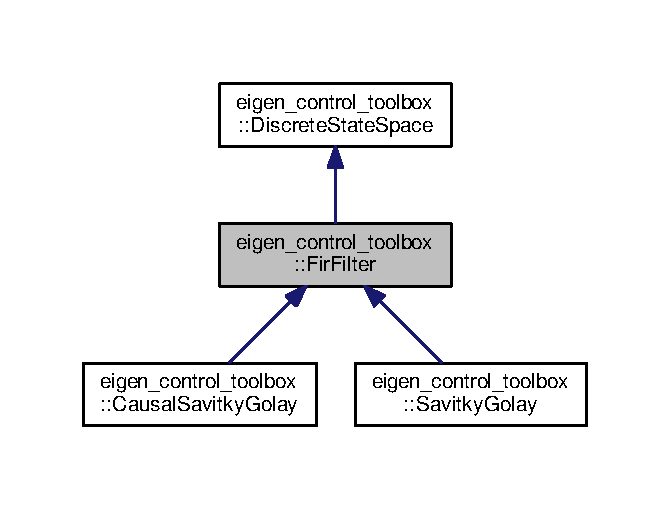
\includegraphics[width=322pt]{classeigen__control__toolbox_1_1_fir_filter__inherit__graph}
\end{center}
\end{figure}


Collaboration diagram for eigen\+\_\+control\+\_\+toolbox\+:\+:Fir\+Filter\+:
\nopagebreak
\begin{figure}[H]
\begin{center}
\leavevmode
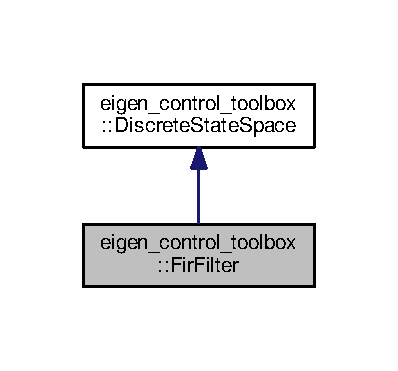
\includegraphics[width=191pt]{classeigen__control__toolbox_1_1_fir_filter__coll__graph}
\end{center}
\end{figure}
\subsection*{Public Member Functions}
\begin{DoxyCompactItemize}
\item 
\hyperlink{classeigen__control__toolbox_1_1_fir_filter_a683d5005efb7f4ed7f1e59a9b35f350a}{Fir\+Filter} ()
\item 
\hyperlink{classeigen__control__toolbox_1_1_fir_filter_a6867a6ffb9e39fc8c88e9d4089978905}{Fir\+Filter} (Eigen\+::\+Matrix\+Xd coeffs)
\item 
void \hyperlink{classeigen__control__toolbox_1_1_fir_filter_a63e7808ced78b8ca9d24c6109d6d6ad4}{compute\+Matrices} (Eigen\+::\+Matrix\+Xd coeffs)
\item 
virtual void \hyperlink{classeigen__control__toolbox_1_1_fir_filter_acb92ff23942f907f54b2259882b60ac1}{set\+State\+From\+IO} (const Eigen\+::\+Ref$<$ Eigen\+::\+Vector\+Xd $>$ past\+\_\+inputs, const Eigen\+::\+Ref$<$ Eigen\+::\+Vector\+Xd $>$ past\+\_\+outputs)
\item 
virtual Eigen\+::\+Vector\+Xd \hyperlink{classeigen__control__toolbox_1_1_fir_filter_a1d6d8cf69bc4dc7dfea62e14cf50375c}{update} (const Eigen\+::\+Ref$<$ Eigen\+::\+Vector\+Xd $>$ input)
\end{DoxyCompactItemize}
\subsection*{Additional Inherited Members}


\subsection{Detailed Description}


Definition at line 8 of file eigen\+\_\+fir\+\_\+filters.\+h.



\subsection{Constructor \& Destructor Documentation}
\index{eigen\+\_\+control\+\_\+toolbox\+::\+Fir\+Filter@{eigen\+\_\+control\+\_\+toolbox\+::\+Fir\+Filter}!Fir\+Filter@{Fir\+Filter}}
\index{Fir\+Filter@{Fir\+Filter}!eigen\+\_\+control\+\_\+toolbox\+::\+Fir\+Filter@{eigen\+\_\+control\+\_\+toolbox\+::\+Fir\+Filter}}
\subsubsection[{\texorpdfstring{Fir\+Filter()}{FirFilter()}}]{\setlength{\rightskip}{0pt plus 5cm}eigen\+\_\+control\+\_\+toolbox\+::\+Fir\+Filter\+::\+Fir\+Filter (
\begin{DoxyParamCaption}
{}
\end{DoxyParamCaption}
)}\hypertarget{classeigen__control__toolbox_1_1_fir_filter_a683d5005efb7f4ed7f1e59a9b35f350a}{}\label{classeigen__control__toolbox_1_1_fir_filter_a683d5005efb7f4ed7f1e59a9b35f350a}


Definition at line 5 of file eigen\+\_\+fir\+\_\+filters.\+cpp.

\index{eigen\+\_\+control\+\_\+toolbox\+::\+Fir\+Filter@{eigen\+\_\+control\+\_\+toolbox\+::\+Fir\+Filter}!Fir\+Filter@{Fir\+Filter}}
\index{Fir\+Filter@{Fir\+Filter}!eigen\+\_\+control\+\_\+toolbox\+::\+Fir\+Filter@{eigen\+\_\+control\+\_\+toolbox\+::\+Fir\+Filter}}
\subsubsection[{\texorpdfstring{Fir\+Filter(\+Eigen\+::\+Matrix\+Xd coeffs)}{FirFilter(Eigen::MatrixXd coeffs)}}]{\setlength{\rightskip}{0pt plus 5cm}eigen\+\_\+control\+\_\+toolbox\+::\+Fir\+Filter\+::\+Fir\+Filter (
\begin{DoxyParamCaption}
\item[{Eigen\+::\+Matrix\+Xd}]{coeffs}
\end{DoxyParamCaption}
)}\hypertarget{classeigen__control__toolbox_1_1_fir_filter_a6867a6ffb9e39fc8c88e9d4089978905}{}\label{classeigen__control__toolbox_1_1_fir_filter_a6867a6ffb9e39fc8c88e9d4089978905}


Definition at line 10 of file eigen\+\_\+fir\+\_\+filters.\+cpp.



\subsection{Member Function Documentation}
\index{eigen\+\_\+control\+\_\+toolbox\+::\+Fir\+Filter@{eigen\+\_\+control\+\_\+toolbox\+::\+Fir\+Filter}!compute\+Matrices@{compute\+Matrices}}
\index{compute\+Matrices@{compute\+Matrices}!eigen\+\_\+control\+\_\+toolbox\+::\+Fir\+Filter@{eigen\+\_\+control\+\_\+toolbox\+::\+Fir\+Filter}}
\subsubsection[{\texorpdfstring{compute\+Matrices(\+Eigen\+::\+Matrix\+Xd coeffs)}{computeMatrices(Eigen::MatrixXd coeffs)}}]{\setlength{\rightskip}{0pt plus 5cm}void eigen\+\_\+control\+\_\+toolbox\+::\+Fir\+Filter\+::compute\+Matrices (
\begin{DoxyParamCaption}
\item[{Eigen\+::\+Matrix\+Xd}]{coeffs}
\end{DoxyParamCaption}
)}\hypertarget{classeigen__control__toolbox_1_1_fir_filter_a63e7808ced78b8ca9d24c6109d6d6ad4}{}\label{classeigen__control__toolbox_1_1_fir_filter_a63e7808ced78b8ca9d24c6109d6d6ad4}


Definition at line 15 of file eigen\+\_\+fir\+\_\+filters.\+cpp.

\index{eigen\+\_\+control\+\_\+toolbox\+::\+Fir\+Filter@{eigen\+\_\+control\+\_\+toolbox\+::\+Fir\+Filter}!set\+State\+From\+IO@{set\+State\+From\+IO}}
\index{set\+State\+From\+IO@{set\+State\+From\+IO}!eigen\+\_\+control\+\_\+toolbox\+::\+Fir\+Filter@{eigen\+\_\+control\+\_\+toolbox\+::\+Fir\+Filter}}
\subsubsection[{\texorpdfstring{set\+State\+From\+I\+O(const Eigen\+::\+Ref$<$ Eigen\+::\+Vector\+Xd $>$ past\+\_\+inputs, const Eigen\+::\+Ref$<$ Eigen\+::\+Vector\+Xd $>$ past\+\_\+outputs)}{setStateFromIO(const Eigen::Ref< Eigen::VectorXd > past_inputs, const Eigen::Ref< Eigen::VectorXd > past_outputs)}}]{\setlength{\rightskip}{0pt plus 5cm}void eigen\+\_\+control\+\_\+toolbox\+::\+Fir\+Filter\+::set\+State\+From\+IO (
\begin{DoxyParamCaption}
\item[{const Eigen\+::\+Ref$<$ Eigen\+::\+Vector\+Xd $>$}]{past\+\_\+inputs, }
\item[{const Eigen\+::\+Ref$<$ Eigen\+::\+Vector\+Xd $>$}]{past\+\_\+outputs}
\end{DoxyParamCaption}
)\hspace{0.3cm}{\ttfamily [virtual]}}\hypertarget{classeigen__control__toolbox_1_1_fir_filter_acb92ff23942f907f54b2259882b60ac1}{}\label{classeigen__control__toolbox_1_1_fir_filter_acb92ff23942f907f54b2259882b60ac1}


Reimplemented from \hyperlink{classeigen__control__toolbox_1_1_discrete_state_space_a5965984530e7b3b915883d9a287e2d14}{eigen\+\_\+control\+\_\+toolbox\+::\+Discrete\+State\+Space}.



Definition at line 48 of file eigen\+\_\+fir\+\_\+filters.\+cpp.

\index{eigen\+\_\+control\+\_\+toolbox\+::\+Fir\+Filter@{eigen\+\_\+control\+\_\+toolbox\+::\+Fir\+Filter}!update@{update}}
\index{update@{update}!eigen\+\_\+control\+\_\+toolbox\+::\+Fir\+Filter@{eigen\+\_\+control\+\_\+toolbox\+::\+Fir\+Filter}}
\subsubsection[{\texorpdfstring{update(const Eigen\+::\+Ref$<$ Eigen\+::\+Vector\+Xd $>$ input)}{update(const Eigen::Ref< Eigen::VectorXd > input)}}]{\setlength{\rightskip}{0pt plus 5cm}Eigen\+::\+Vector\+Xd eigen\+\_\+control\+\_\+toolbox\+::\+Fir\+Filter\+::update (
\begin{DoxyParamCaption}
\item[{const Eigen\+::\+Ref$<$ Eigen\+::\+Vector\+Xd $>$}]{input}
\end{DoxyParamCaption}
)\hspace{0.3cm}{\ttfamily [virtual]}}\hypertarget{classeigen__control__toolbox_1_1_fir_filter_a1d6d8cf69bc4dc7dfea62e14cf50375c}{}\label{classeigen__control__toolbox_1_1_fir_filter_a1d6d8cf69bc4dc7dfea62e14cf50375c}


Reimplemented from \hyperlink{classeigen__control__toolbox_1_1_discrete_state_space_ae58e06527268253cea809554a528fdfe}{eigen\+\_\+control\+\_\+toolbox\+::\+Discrete\+State\+Space}.



Definition at line 36 of file eigen\+\_\+fir\+\_\+filters.\+cpp.



The documentation for this class was generated from the following files\+:\begin{DoxyCompactItemize}
\item 
include/eigen\+\_\+state\+\_\+space\+\_\+systems/\hyperlink{eigen__fir__filters_8h}{eigen\+\_\+fir\+\_\+filters.\+h}\item 
src/eigen\+\_\+state\+\_\+space\+\_\+systems/\hyperlink{eigen__fir__filters_8cpp}{eigen\+\_\+fir\+\_\+filters.\+cpp}\end{DoxyCompactItemize}

\hypertarget{classeigen__control__toolbox_1_1_first_order_high_pass}{}\section{eigen\+\_\+control\+\_\+toolbox\+:\+:First\+Order\+High\+Pass Class Reference}
\label{classeigen__control__toolbox_1_1_first_order_high_pass}\index{eigen\+\_\+control\+\_\+toolbox\+::\+First\+Order\+High\+Pass@{eigen\+\_\+control\+\_\+toolbox\+::\+First\+Order\+High\+Pass}}


{\ttfamily \#include $<$eigen\+\_\+iir\+\_\+filters.\+h$>$}



Inheritance diagram for eigen\+\_\+control\+\_\+toolbox\+:\+:First\+Order\+High\+Pass\+:
\nopagebreak
\begin{figure}[H]
\begin{center}
\leavevmode
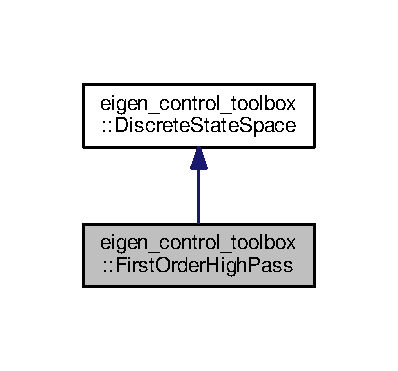
\includegraphics[width=191pt]{classeigen__control__toolbox_1_1_first_order_high_pass__inherit__graph}
\end{center}
\end{figure}


Collaboration diagram for eigen\+\_\+control\+\_\+toolbox\+:\+:First\+Order\+High\+Pass\+:
\nopagebreak
\begin{figure}[H]
\begin{center}
\leavevmode
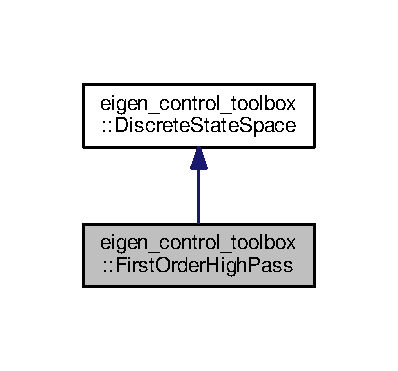
\includegraphics[width=191pt]{classeigen__control__toolbox_1_1_first_order_high_pass__coll__graph}
\end{center}
\end{figure}
\subsection*{Public Member Functions}
\begin{DoxyCompactItemize}
\item 
\hyperlink{classeigen__control__toolbox_1_1_first_order_high_pass_accf62cc2f6f2542d0baecaa61de980d4}{First\+Order\+High\+Pass} (const double \&natural\+\_\+frequency, const double \&sample\+\_\+period)
\end{DoxyCompactItemize}
\subsection*{Additional Inherited Members}


\subsection{Detailed Description}


Definition at line 19 of file eigen\+\_\+iir\+\_\+filters.\+h.



\subsection{Constructor \& Destructor Documentation}
\index{eigen\+\_\+control\+\_\+toolbox\+::\+First\+Order\+High\+Pass@{eigen\+\_\+control\+\_\+toolbox\+::\+First\+Order\+High\+Pass}!First\+Order\+High\+Pass@{First\+Order\+High\+Pass}}
\index{First\+Order\+High\+Pass@{First\+Order\+High\+Pass}!eigen\+\_\+control\+\_\+toolbox\+::\+First\+Order\+High\+Pass@{eigen\+\_\+control\+\_\+toolbox\+::\+First\+Order\+High\+Pass}}
\subsubsection[{\texorpdfstring{First\+Order\+High\+Pass(const double \&natural\+\_\+frequency, const double \&sample\+\_\+period)}{FirstOrderHighPass(const double &natural_frequency, const double &sample_period)}}]{\setlength{\rightskip}{0pt plus 5cm}eigen\+\_\+control\+\_\+toolbox\+::\+First\+Order\+High\+Pass\+::\+First\+Order\+High\+Pass (
\begin{DoxyParamCaption}
\item[{const double \&}]{natural\+\_\+frequency, }
\item[{const double \&}]{sample\+\_\+period}
\end{DoxyParamCaption}
)}\hypertarget{classeigen__control__toolbox_1_1_first_order_high_pass_accf62cc2f6f2542d0baecaa61de980d4}{}\label{classeigen__control__toolbox_1_1_first_order_high_pass_accf62cc2f6f2542d0baecaa61de980d4}


Definition at line 24 of file eigen\+\_\+iir\+\_\+filters.\+cpp.



The documentation for this class was generated from the following files\+:\begin{DoxyCompactItemize}
\item 
include/eigen\+\_\+state\+\_\+space\+\_\+systems/\hyperlink{eigen__iir__filters_8h}{eigen\+\_\+iir\+\_\+filters.\+h}\item 
src/eigen\+\_\+state\+\_\+space\+\_\+systems/\hyperlink{eigen__iir__filters_8cpp}{eigen\+\_\+iir\+\_\+filters.\+cpp}\end{DoxyCompactItemize}

\hypertarget{classeigen__control__toolbox_1_1_first_order_low_pass}{}\section{eigen\+\_\+control\+\_\+toolbox\+:\+:First\+Order\+Low\+Pass Class Reference}
\label{classeigen__control__toolbox_1_1_first_order_low_pass}\index{eigen\+\_\+control\+\_\+toolbox\+::\+First\+Order\+Low\+Pass@{eigen\+\_\+control\+\_\+toolbox\+::\+First\+Order\+Low\+Pass}}


{\ttfamily \#include $<$eigen\+\_\+iir\+\_\+filters.\+h$>$}



Inheritance diagram for eigen\+\_\+control\+\_\+toolbox\+:\+:First\+Order\+Low\+Pass\+:
\nopagebreak
\begin{figure}[H]
\begin{center}
\leavevmode
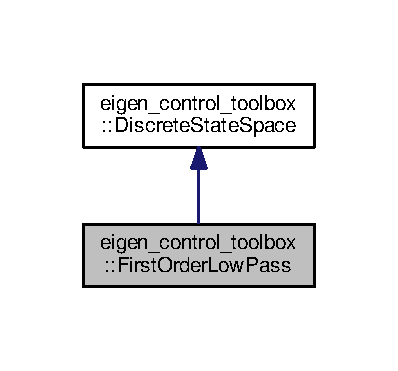
\includegraphics[width=191pt]{classeigen__control__toolbox_1_1_first_order_low_pass__inherit__graph}
\end{center}
\end{figure}


Collaboration diagram for eigen\+\_\+control\+\_\+toolbox\+:\+:First\+Order\+Low\+Pass\+:
\nopagebreak
\begin{figure}[H]
\begin{center}
\leavevmode
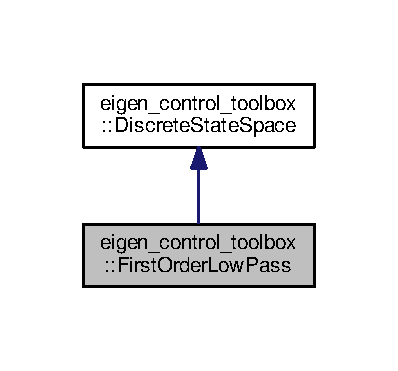
\includegraphics[width=191pt]{classeigen__control__toolbox_1_1_first_order_low_pass__coll__graph}
\end{center}
\end{figure}
\subsection*{Public Member Functions}
\begin{DoxyCompactItemize}
\item 
\hyperlink{classeigen__control__toolbox_1_1_first_order_low_pass_a84ce9dcb1d6a787f96fbf0d4b76e22fe}{First\+Order\+Low\+Pass} (const double \&natural\+\_\+frequency, const double \&sample\+\_\+period)
\end{DoxyCompactItemize}
\subsection*{Additional Inherited Members}


\subsection{Detailed Description}


Definition at line 12 of file eigen\+\_\+iir\+\_\+filters.\+h.



\subsection{Constructor \& Destructor Documentation}
\index{eigen\+\_\+control\+\_\+toolbox\+::\+First\+Order\+Low\+Pass@{eigen\+\_\+control\+\_\+toolbox\+::\+First\+Order\+Low\+Pass}!First\+Order\+Low\+Pass@{First\+Order\+Low\+Pass}}
\index{First\+Order\+Low\+Pass@{First\+Order\+Low\+Pass}!eigen\+\_\+control\+\_\+toolbox\+::\+First\+Order\+Low\+Pass@{eigen\+\_\+control\+\_\+toolbox\+::\+First\+Order\+Low\+Pass}}
\subsubsection[{\texorpdfstring{First\+Order\+Low\+Pass(const double \&natural\+\_\+frequency, const double \&sample\+\_\+period)}{FirstOrderLowPass(const double &natural_frequency, const double &sample_period)}}]{\setlength{\rightskip}{0pt plus 5cm}eigen\+\_\+control\+\_\+toolbox\+::\+First\+Order\+Low\+Pass\+::\+First\+Order\+Low\+Pass (
\begin{DoxyParamCaption}
\item[{const double \&}]{natural\+\_\+frequency, }
\item[{const double \&}]{sample\+\_\+period}
\end{DoxyParamCaption}
)}\hypertarget{classeigen__control__toolbox_1_1_first_order_low_pass_a84ce9dcb1d6a787f96fbf0d4b76e22fe}{}\label{classeigen__control__toolbox_1_1_first_order_low_pass_a84ce9dcb1d6a787f96fbf0d4b76e22fe}


Definition at line 5 of file eigen\+\_\+iir\+\_\+filters.\+cpp.



The documentation for this class was generated from the following files\+:\begin{DoxyCompactItemize}
\item 
include/eigen\+\_\+state\+\_\+space\+\_\+systems/\hyperlink{eigen__iir__filters_8h}{eigen\+\_\+iir\+\_\+filters.\+h}\item 
src/eigen\+\_\+state\+\_\+space\+\_\+systems/\hyperlink{eigen__iir__filters_8cpp}{eigen\+\_\+iir\+\_\+filters.\+cpp}\end{DoxyCompactItemize}

\hypertarget{classeigen__control__toolbox_1_1_savitky_golay}{}\section{eigen\+\_\+control\+\_\+toolbox\+:\+:Savitky\+Golay Class Reference}
\label{classeigen__control__toolbox_1_1_savitky_golay}\index{eigen\+\_\+control\+\_\+toolbox\+::\+Savitky\+Golay@{eigen\+\_\+control\+\_\+toolbox\+::\+Savitky\+Golay}}


{\ttfamily \#include $<$eigen\+\_\+sg\+\_\+filter.\+h$>$}



Inheritance diagram for eigen\+\_\+control\+\_\+toolbox\+:\+:Savitky\+Golay\+:
\nopagebreak
\begin{figure}[H]
\begin{center}
\leavevmode
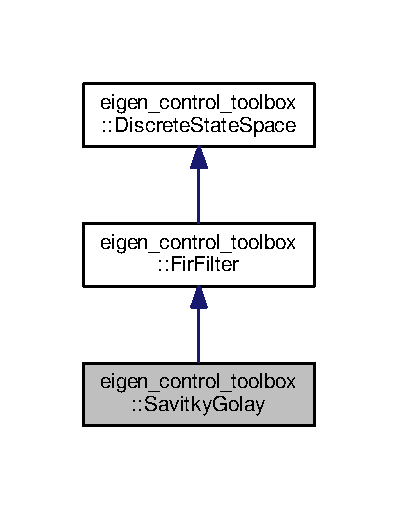
\includegraphics[width=191pt]{classeigen__control__toolbox_1_1_savitky_golay__inherit__graph}
\end{center}
\end{figure}


Collaboration diagram for eigen\+\_\+control\+\_\+toolbox\+:\+:Savitky\+Golay\+:
\nopagebreak
\begin{figure}[H]
\begin{center}
\leavevmode
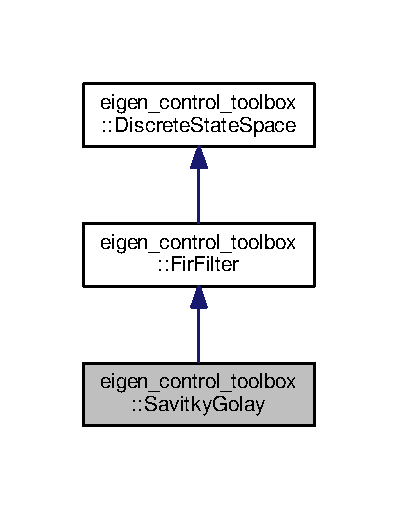
\includegraphics[width=191pt]{classeigen__control__toolbox_1_1_savitky_golay__coll__graph}
\end{center}
\end{figure}
\subsection*{Public Member Functions}
\begin{DoxyCompactItemize}
\item 
\hyperlink{classeigen__control__toolbox_1_1_savitky_golay_a93b69082ddae291c2d6e12670fe91d68}{Savitky\+Golay} ()
\item 
\hyperlink{classeigen__control__toolbox_1_1_savitky_golay_a46eafa63bbe9866f323f2394c72ac998}{Savitky\+Golay} (const double \&natural\+\_\+frequency, const double \&sample\+\_\+period, const unsigned int \&polynomial\+\_\+order, const unsigned int \&output\+\_\+size)
\item 
\hyperlink{classeigen__control__toolbox_1_1_savitky_golay_acaa769bb795a34c2ec4bd5857e6c0923}{Savitky\+Golay} (const unsigned int \&window, const double \&sample\+\_\+period, const unsigned int \&polynomial\+\_\+order, const unsigned int \&output\+\_\+size)
\end{DoxyCompactItemize}
\subsection*{Protected Member Functions}
\begin{DoxyCompactItemize}
\item 
void \hyperlink{classeigen__control__toolbox_1_1_savitky_golay_ae1767a408504913880b7c742eb4e4831}{compute\+Coeffs} (const unsigned int \&polynomial\+\_\+order, const unsigned int \&window, const unsigned int \&output\+\_\+size)
\item 
void \hyperlink{classeigen__control__toolbox_1_1_savitky_golay_a499c308c1672cedc332e92116257c673}{init\+Savitky\+Golay} (const double \&natural\+\_\+frequency, const double \&sample\+\_\+period, const unsigned int \&polynomial\+\_\+order, const unsigned int \&output\+\_\+size=1)
\item 
void \hyperlink{classeigen__control__toolbox_1_1_savitky_golay_a9b0b89e15d57b7737c01610d1e5e7c4c}{init\+Savitky\+Golay} (const unsigned int \&window, const double \&sample\+\_\+period, const unsigned int \&polynomial\+\_\+order, const unsigned int \&output\+\_\+size=1)
\end{DoxyCompactItemize}
\subsection*{Additional Inherited Members}


\subsection{Detailed Description}


Definition at line 9 of file eigen\+\_\+sg\+\_\+filter.\+h.



\subsection{Constructor \& Destructor Documentation}
\index{eigen\+\_\+control\+\_\+toolbox\+::\+Savitky\+Golay@{eigen\+\_\+control\+\_\+toolbox\+::\+Savitky\+Golay}!Savitky\+Golay@{Savitky\+Golay}}
\index{Savitky\+Golay@{Savitky\+Golay}!eigen\+\_\+control\+\_\+toolbox\+::\+Savitky\+Golay@{eigen\+\_\+control\+\_\+toolbox\+::\+Savitky\+Golay}}
\subsubsection[{\texorpdfstring{Savitky\+Golay()}{SavitkyGolay()}}]{\setlength{\rightskip}{0pt plus 5cm}eigen\+\_\+control\+\_\+toolbox\+::\+Savitky\+Golay\+::\+Savitky\+Golay (
\begin{DoxyParamCaption}
{}
\end{DoxyParamCaption}
)\hspace{0.3cm}{\ttfamily [inline]}}\hypertarget{classeigen__control__toolbox_1_1_savitky_golay_a93b69082ddae291c2d6e12670fe91d68}{}\label{classeigen__control__toolbox_1_1_savitky_golay_a93b69082ddae291c2d6e12670fe91d68}


Definition at line 31 of file eigen\+\_\+sg\+\_\+filter.\+h.

\index{eigen\+\_\+control\+\_\+toolbox\+::\+Savitky\+Golay@{eigen\+\_\+control\+\_\+toolbox\+::\+Savitky\+Golay}!Savitky\+Golay@{Savitky\+Golay}}
\index{Savitky\+Golay@{Savitky\+Golay}!eigen\+\_\+control\+\_\+toolbox\+::\+Savitky\+Golay@{eigen\+\_\+control\+\_\+toolbox\+::\+Savitky\+Golay}}
\subsubsection[{\texorpdfstring{Savitky\+Golay(const double \&natural\+\_\+frequency, const double \&sample\+\_\+period, const unsigned int \&polynomial\+\_\+order, const unsigned int \&output\+\_\+size)}{SavitkyGolay(const double &natural_frequency, const double &sample_period, const unsigned int &polynomial_order, const unsigned int &output_size)}}]{\setlength{\rightskip}{0pt plus 5cm}eigen\+\_\+control\+\_\+toolbox\+::\+Savitky\+Golay\+::\+Savitky\+Golay (
\begin{DoxyParamCaption}
\item[{const double \&}]{natural\+\_\+frequency, }
\item[{const double \&}]{sample\+\_\+period, }
\item[{const unsigned int \&}]{polynomial\+\_\+order, }
\item[{const unsigned int \&}]{output\+\_\+size}
\end{DoxyParamCaption}
)}\hypertarget{classeigen__control__toolbox_1_1_savitky_golay_a46eafa63bbe9866f323f2394c72ac998}{}\label{classeigen__control__toolbox_1_1_savitky_golay_a46eafa63bbe9866f323f2394c72ac998}


Definition at line 6 of file eigen\+\_\+sg\+\_\+filter.\+cpp.

\index{eigen\+\_\+control\+\_\+toolbox\+::\+Savitky\+Golay@{eigen\+\_\+control\+\_\+toolbox\+::\+Savitky\+Golay}!Savitky\+Golay@{Savitky\+Golay}}
\index{Savitky\+Golay@{Savitky\+Golay}!eigen\+\_\+control\+\_\+toolbox\+::\+Savitky\+Golay@{eigen\+\_\+control\+\_\+toolbox\+::\+Savitky\+Golay}}
\subsubsection[{\texorpdfstring{Savitky\+Golay(const unsigned int \&window, const double \&sample\+\_\+period, const unsigned int \&polynomial\+\_\+order, const unsigned int \&output\+\_\+size)}{SavitkyGolay(const unsigned int &window, const double &sample_period, const unsigned int &polynomial_order, const unsigned int &output_size)}}]{\setlength{\rightskip}{0pt plus 5cm}eigen\+\_\+control\+\_\+toolbox\+::\+Savitky\+Golay\+::\+Savitky\+Golay (
\begin{DoxyParamCaption}
\item[{const unsigned int \&}]{window, }
\item[{const double \&}]{sample\+\_\+period, }
\item[{const unsigned int \&}]{polynomial\+\_\+order, }
\item[{const unsigned int \&}]{output\+\_\+size}
\end{DoxyParamCaption}
)}\hypertarget{classeigen__control__toolbox_1_1_savitky_golay_acaa769bb795a34c2ec4bd5857e6c0923}{}\label{classeigen__control__toolbox_1_1_savitky_golay_acaa769bb795a34c2ec4bd5857e6c0923}


Definition at line 15 of file eigen\+\_\+sg\+\_\+filter.\+cpp.



\subsection{Member Function Documentation}
\index{eigen\+\_\+control\+\_\+toolbox\+::\+Savitky\+Golay@{eigen\+\_\+control\+\_\+toolbox\+::\+Savitky\+Golay}!compute\+Coeffs@{compute\+Coeffs}}
\index{compute\+Coeffs@{compute\+Coeffs}!eigen\+\_\+control\+\_\+toolbox\+::\+Savitky\+Golay@{eigen\+\_\+control\+\_\+toolbox\+::\+Savitky\+Golay}}
\subsubsection[{\texorpdfstring{compute\+Coeffs(const unsigned int \&polynomial\+\_\+order, const unsigned int \&window, const unsigned int \&output\+\_\+size)}{computeCoeffs(const unsigned int &polynomial_order, const unsigned int &window, const unsigned int &output_size)}}]{\setlength{\rightskip}{0pt plus 5cm}void eigen\+\_\+control\+\_\+toolbox\+::\+Savitky\+Golay\+::compute\+Coeffs (
\begin{DoxyParamCaption}
\item[{const unsigned int \&}]{polynomial\+\_\+order, }
\item[{const unsigned int \&}]{window, }
\item[{const unsigned int \&}]{output\+\_\+size}
\end{DoxyParamCaption}
)\hspace{0.3cm}{\ttfamily [protected]}}\hypertarget{classeigen__control__toolbox_1_1_savitky_golay_ae1767a408504913880b7c742eb4e4831}{}\label{classeigen__control__toolbox_1_1_savitky_golay_ae1767a408504913880b7c742eb4e4831}


Definition at line 46 of file eigen\+\_\+sg\+\_\+filter.\+cpp.

\index{eigen\+\_\+control\+\_\+toolbox\+::\+Savitky\+Golay@{eigen\+\_\+control\+\_\+toolbox\+::\+Savitky\+Golay}!init\+Savitky\+Golay@{init\+Savitky\+Golay}}
\index{init\+Savitky\+Golay@{init\+Savitky\+Golay}!eigen\+\_\+control\+\_\+toolbox\+::\+Savitky\+Golay@{eigen\+\_\+control\+\_\+toolbox\+::\+Savitky\+Golay}}
\subsubsection[{\texorpdfstring{init\+Savitky\+Golay(const double \&natural\+\_\+frequency, const double \&sample\+\_\+period, const unsigned int \&polynomial\+\_\+order, const unsigned int \&output\+\_\+size=1)}{initSavitkyGolay(const double &natural_frequency, const double &sample_period, const unsigned int &polynomial_order, const unsigned int &output_size=1)}}]{\setlength{\rightskip}{0pt plus 5cm}void eigen\+\_\+control\+\_\+toolbox\+::\+Savitky\+Golay\+::init\+Savitky\+Golay (
\begin{DoxyParamCaption}
\item[{const double \&}]{natural\+\_\+frequency, }
\item[{const double \&}]{sample\+\_\+period, }
\item[{const unsigned int \&}]{polynomial\+\_\+order, }
\item[{const unsigned int \&}]{output\+\_\+size = {\ttfamily 1}}
\end{DoxyParamCaption}
)\hspace{0.3cm}{\ttfamily [protected]}}\hypertarget{classeigen__control__toolbox_1_1_savitky_golay_a499c308c1672cedc332e92116257c673}{}\label{classeigen__control__toolbox_1_1_savitky_golay_a499c308c1672cedc332e92116257c673}


Definition at line 20 of file eigen\+\_\+sg\+\_\+filter.\+cpp.

\index{eigen\+\_\+control\+\_\+toolbox\+::\+Savitky\+Golay@{eigen\+\_\+control\+\_\+toolbox\+::\+Savitky\+Golay}!init\+Savitky\+Golay@{init\+Savitky\+Golay}}
\index{init\+Savitky\+Golay@{init\+Savitky\+Golay}!eigen\+\_\+control\+\_\+toolbox\+::\+Savitky\+Golay@{eigen\+\_\+control\+\_\+toolbox\+::\+Savitky\+Golay}}
\subsubsection[{\texorpdfstring{init\+Savitky\+Golay(const unsigned int \&window, const double \&sample\+\_\+period, const unsigned int \&polynomial\+\_\+order, const unsigned int \&output\+\_\+size=1)}{initSavitkyGolay(const unsigned int &window, const double &sample_period, const unsigned int &polynomial_order, const unsigned int &output_size=1)}}]{\setlength{\rightskip}{0pt plus 5cm}void eigen\+\_\+control\+\_\+toolbox\+::\+Savitky\+Golay\+::init\+Savitky\+Golay (
\begin{DoxyParamCaption}
\item[{const unsigned int \&}]{window, }
\item[{const double \&}]{sample\+\_\+period, }
\item[{const unsigned int \&}]{polynomial\+\_\+order, }
\item[{const unsigned int \&}]{output\+\_\+size = {\ttfamily 1}}
\end{DoxyParamCaption}
)\hspace{0.3cm}{\ttfamily [protected]}}\hypertarget{classeigen__control__toolbox_1_1_savitky_golay_a9b0b89e15d57b7737c01610d1e5e7c4c}{}\label{classeigen__control__toolbox_1_1_savitky_golay_a9b0b89e15d57b7737c01610d1e5e7c4c}


Definition at line 37 of file eigen\+\_\+sg\+\_\+filter.\+cpp.



The documentation for this class was generated from the following files\+:\begin{DoxyCompactItemize}
\item 
include/eigen\+\_\+state\+\_\+space\+\_\+systems/\hyperlink{eigen__sg__filter_8h}{eigen\+\_\+sg\+\_\+filter.\+h}\item 
src/eigen\+\_\+state\+\_\+space\+\_\+systems/\hyperlink{eigen__sg__filter_8cpp}{eigen\+\_\+sg\+\_\+filter.\+cpp}\end{DoxyCompactItemize}

\chapter{File Documentation}
\hypertarget{eigen__common__filters_8h}{}\section{include/eigen\+\_\+state\+\_\+space\+\_\+systems/eigen\+\_\+common\+\_\+filters.h File Reference}
\label{eigen__common__filters_8h}\index{include/eigen\+\_\+state\+\_\+space\+\_\+systems/eigen\+\_\+common\+\_\+filters.\+h@{include/eigen\+\_\+state\+\_\+space\+\_\+systems/eigen\+\_\+common\+\_\+filters.\+h}}
{\ttfamily \#include $<$eigen\+\_\+state\+\_\+space\+\_\+systems/eigen\+\_\+fir\+\_\+filters.\+h$>$}\\*
{\ttfamily \#include $<$eigen\+\_\+state\+\_\+space\+\_\+systems/eigen\+\_\+iir\+\_\+filters.\+h$>$}\\*
{\ttfamily \#include $<$eigen\+\_\+state\+\_\+space\+\_\+systems/eigen\+\_\+sg\+\_\+filter.\+h$>$}\\*
Include dependency graph for eigen\+\_\+common\+\_\+filters.\+h\+:
\nopagebreak
\begin{figure}[H]
\begin{center}
\leavevmode
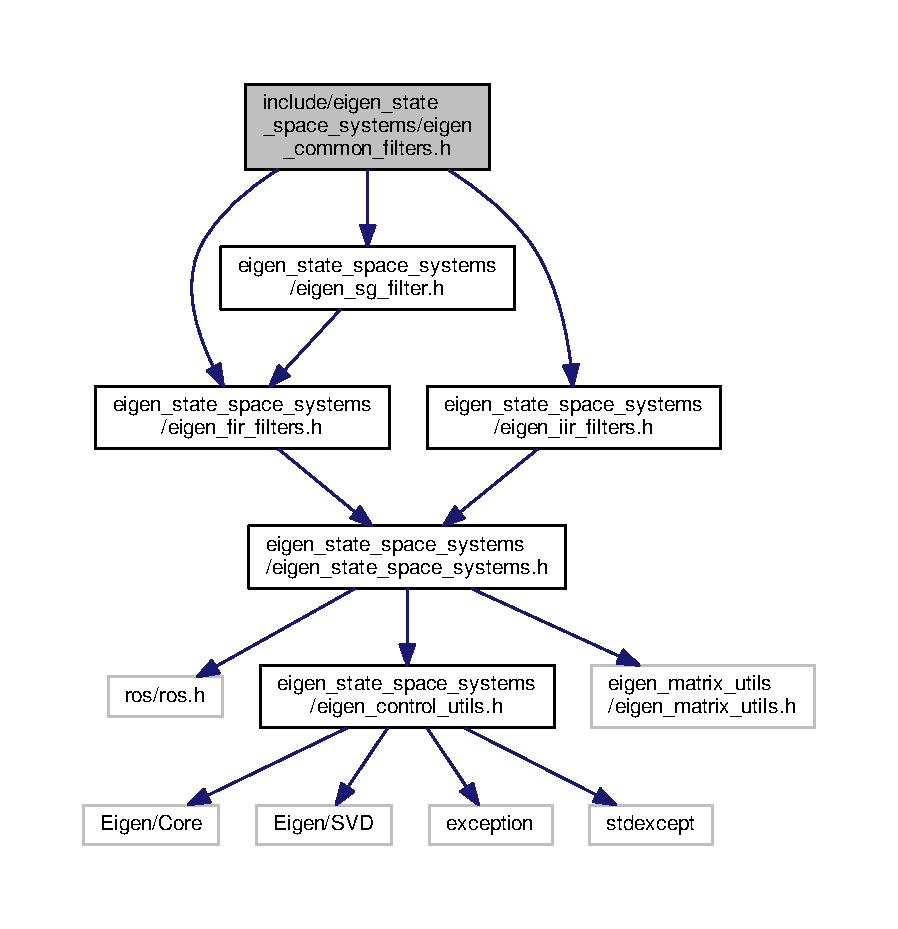
\includegraphics[width=350pt]{eigen__common__filters_8h__incl}
\end{center}
\end{figure}
This graph shows which files directly or indirectly include this file\+:
\nopagebreak
\begin{figure}[H]
\begin{center}
\leavevmode
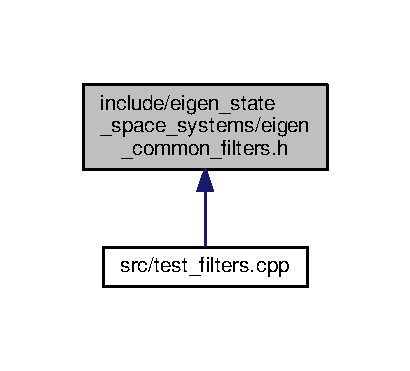
\includegraphics[width=197pt]{eigen__common__filters_8h__dep__incl}
\end{center}
\end{figure}

\hypertarget{eigen__control__utils_8h}{}\section{include/eigen\+\_\+state\+\_\+space\+\_\+systems/eigen\+\_\+control\+\_\+utils.h File Reference}
\label{eigen__control__utils_8h}\index{include/eigen\+\_\+state\+\_\+space\+\_\+systems/eigen\+\_\+control\+\_\+utils.\+h@{include/eigen\+\_\+state\+\_\+space\+\_\+systems/eigen\+\_\+control\+\_\+utils.\+h}}
{\ttfamily \#include $<$Eigen/\+Core$>$}\\*
{\ttfamily \#include $<$Eigen/\+S\+VD$>$}\\*
{\ttfamily \#include $<$exception$>$}\\*
{\ttfamily \#include $<$stdexcept$>$}\\*
Include dependency graph for eigen\+\_\+control\+\_\+utils.\+h\+:
\nopagebreak
\begin{figure}[H]
\begin{center}
\leavevmode
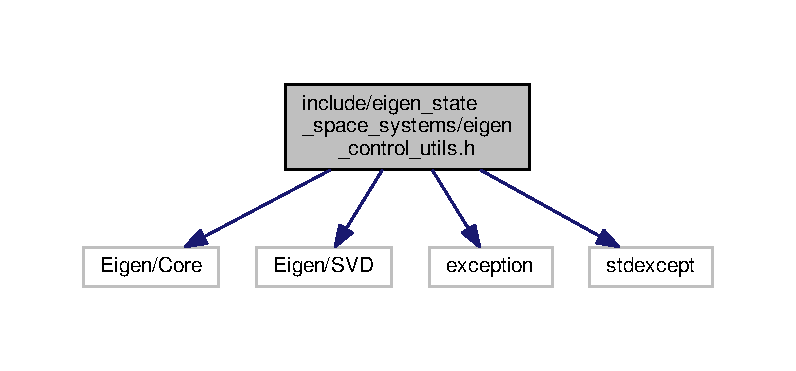
\includegraphics[width=350pt]{eigen__control__utils_8h__incl}
\end{center}
\end{figure}
This graph shows which files directly or indirectly include this file\+:
\nopagebreak
\begin{figure}[H]
\begin{center}
\leavevmode
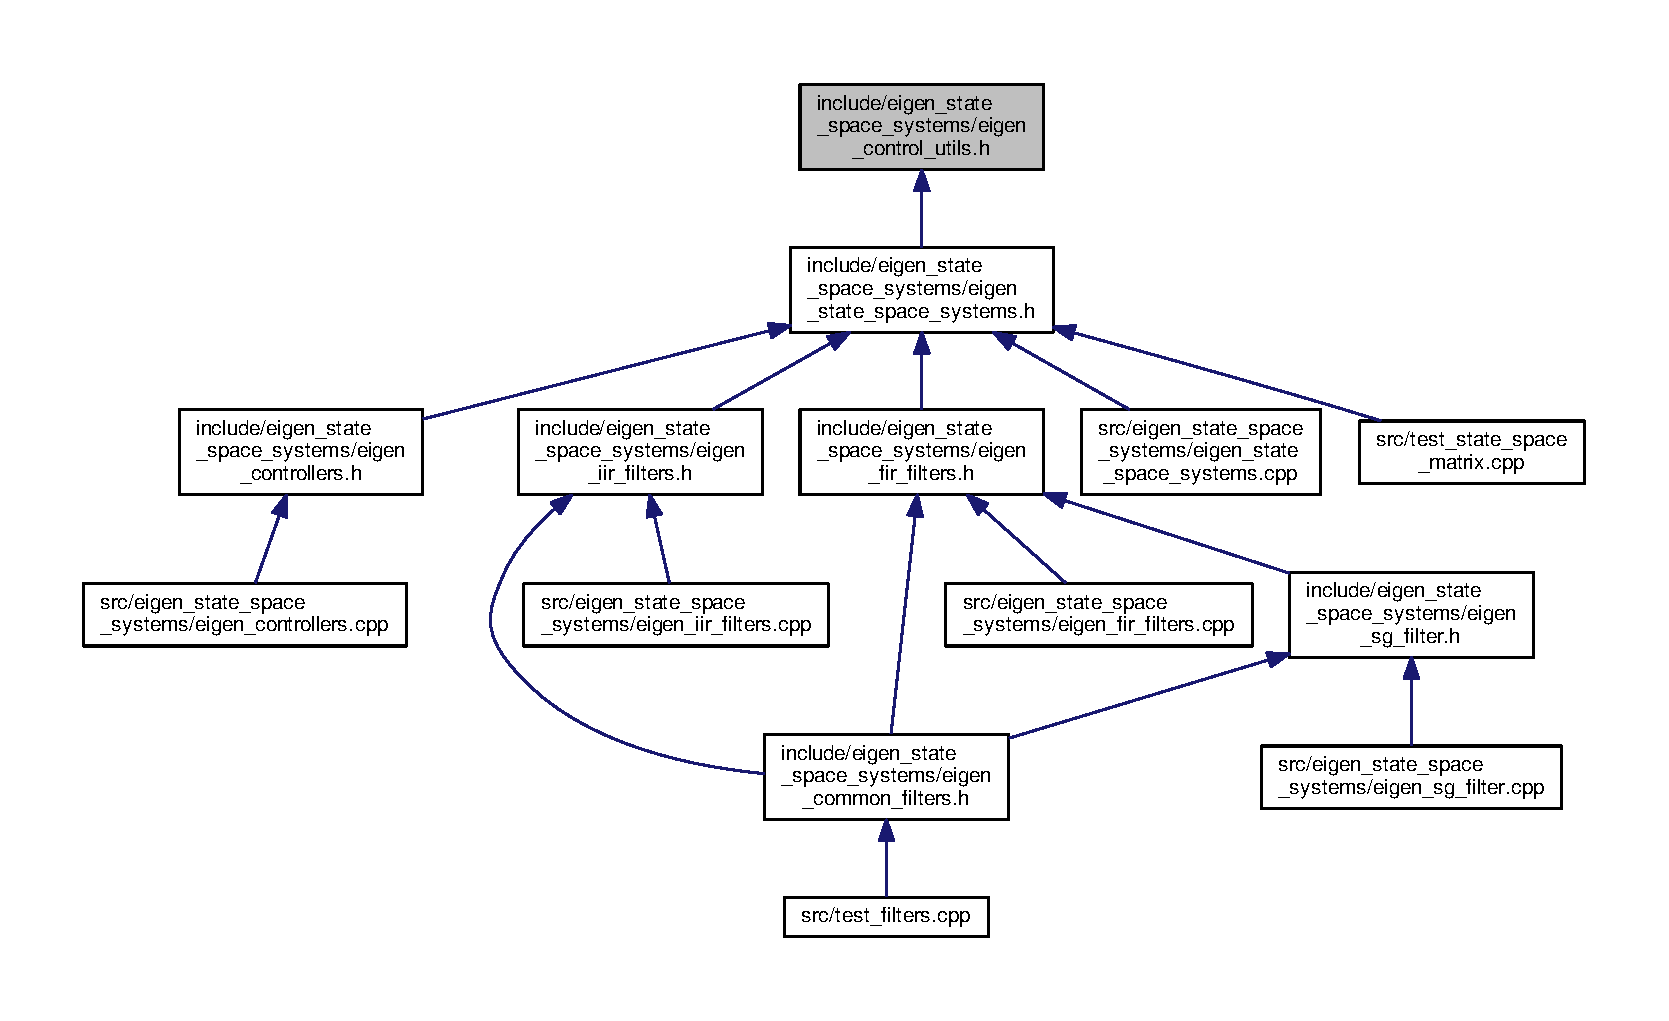
\includegraphics[width=350pt]{eigen__control__utils_8h__dep__incl}
\end{center}
\end{figure}
\subsection*{Namespaces}
\begin{DoxyCompactItemize}
\item 
 \hyperlink{namespaceeigen__control__toolbox}{eigen\+\_\+control\+\_\+toolbox}
\end{DoxyCompactItemize}
\subsection*{Functions}
\begin{DoxyCompactItemize}
\item 
Eigen\+::\+Matrix\+Xd \hyperlink{namespaceeigen__control__toolbox_a86a3c3ab74553e088a86fd855157e2bb}{eigen\+\_\+control\+\_\+toolbox\+::compute\+Observatibility\+Matrix} (const Eigen\+::\+Ref$<$ Eigen\+::\+Matrix\+Xd $>$ A, const Eigen\+::\+Ref$<$ Eigen\+::\+Matrix\+Xd $>$ C)
\item 
Eigen\+::\+Matrix\+Xd \hyperlink{namespaceeigen__control__toolbox_a620ee7eb85ebeea2ca6ec84f96a16ca4}{eigen\+\_\+control\+\_\+toolbox\+::compute\+Input\+To\+Output\+Matrix} (const Eigen\+::\+Ref$<$ Eigen\+::\+Matrix\+Xd $>$ A, const Eigen\+::\+Ref$<$ Eigen\+::\+Matrix\+Xd $>$ B, const Eigen\+::\+Ref$<$ Eigen\+::\+Matrix\+Xd $>$ C, const Eigen\+::\+Ref$<$ Eigen\+::\+Matrix\+Xd $>$ D)
\end{DoxyCompactItemize}

\hypertarget{eigen__controllers_8h}{}\section{include/eigen\+\_\+state\+\_\+space\+\_\+systems/eigen\+\_\+controllers.h File Reference}
\label{eigen__controllers_8h}\index{include/eigen\+\_\+state\+\_\+space\+\_\+systems/eigen\+\_\+controllers.\+h@{include/eigen\+\_\+state\+\_\+space\+\_\+systems/eigen\+\_\+controllers.\+h}}
{\ttfamily \#include $<$eigen\+\_\+state\+\_\+space\+\_\+systems/eigen\+\_\+state\+\_\+space\+\_\+systems.\+h$>$}\\*
Include dependency graph for eigen\+\_\+controllers.\+h\+:
\nopagebreak
\begin{figure}[H]
\begin{center}
\leavevmode
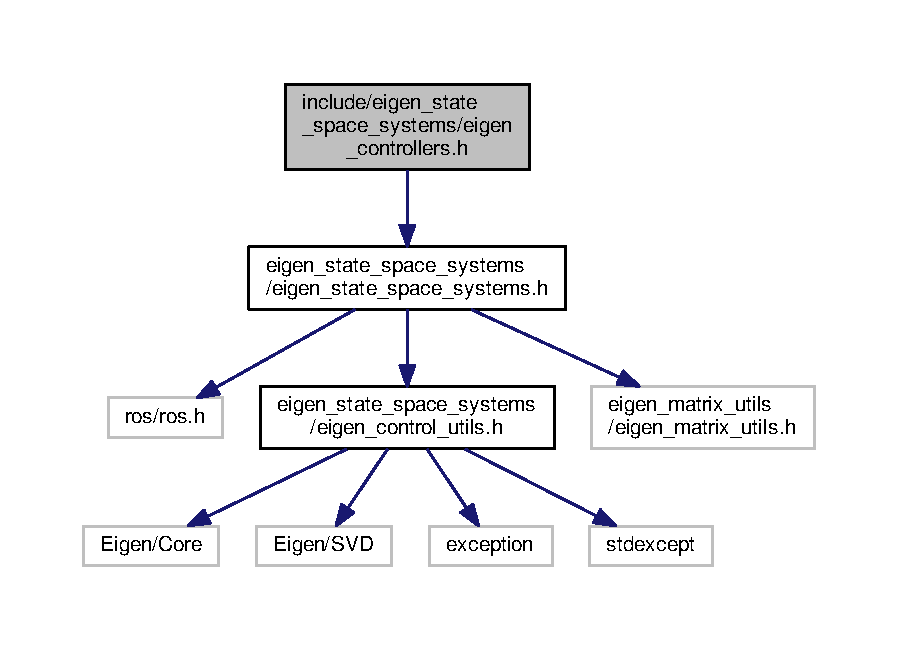
\includegraphics[width=350pt]{eigen__controllers_8h__incl}
\end{center}
\end{figure}
This graph shows which files directly or indirectly include this file\+:
\nopagebreak
\begin{figure}[H]
\begin{center}
\leavevmode
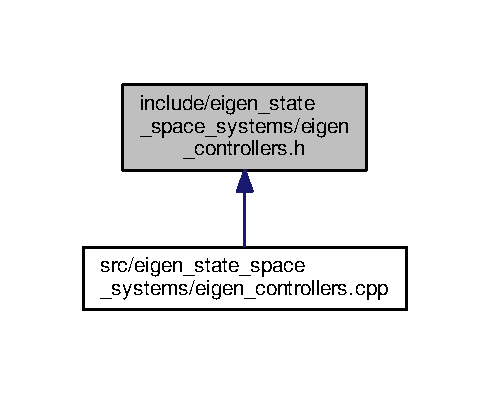
\includegraphics[width=235pt]{eigen__controllers_8h__dep__incl}
\end{center}
\end{figure}
\subsection*{Classes}
\begin{DoxyCompactItemize}
\item 
class \hyperlink{classeigen__control__toolbox_1_1_controller}{eigen\+\_\+control\+\_\+toolbox\+::\+Controller}
\end{DoxyCompactItemize}
\subsection*{Namespaces}
\begin{DoxyCompactItemize}
\item 
 \hyperlink{namespaceeigen__control__toolbox}{eigen\+\_\+control\+\_\+toolbox}
\end{DoxyCompactItemize}

\hypertarget{eigen__fir__filters_8h}{}\section{include/eigen\+\_\+state\+\_\+space\+\_\+systems/eigen\+\_\+fir\+\_\+filters.h File Reference}
\label{eigen__fir__filters_8h}\index{include/eigen\+\_\+state\+\_\+space\+\_\+systems/eigen\+\_\+fir\+\_\+filters.\+h@{include/eigen\+\_\+state\+\_\+space\+\_\+systems/eigen\+\_\+fir\+\_\+filters.\+h}}
{\ttfamily \#include $<$eigen\+\_\+state\+\_\+space\+\_\+systems/eigen\+\_\+state\+\_\+space\+\_\+systems.\+h$>$}\\*
Include dependency graph for eigen\+\_\+fir\+\_\+filters.\+h\+:
\nopagebreak
\begin{figure}[H]
\begin{center}
\leavevmode
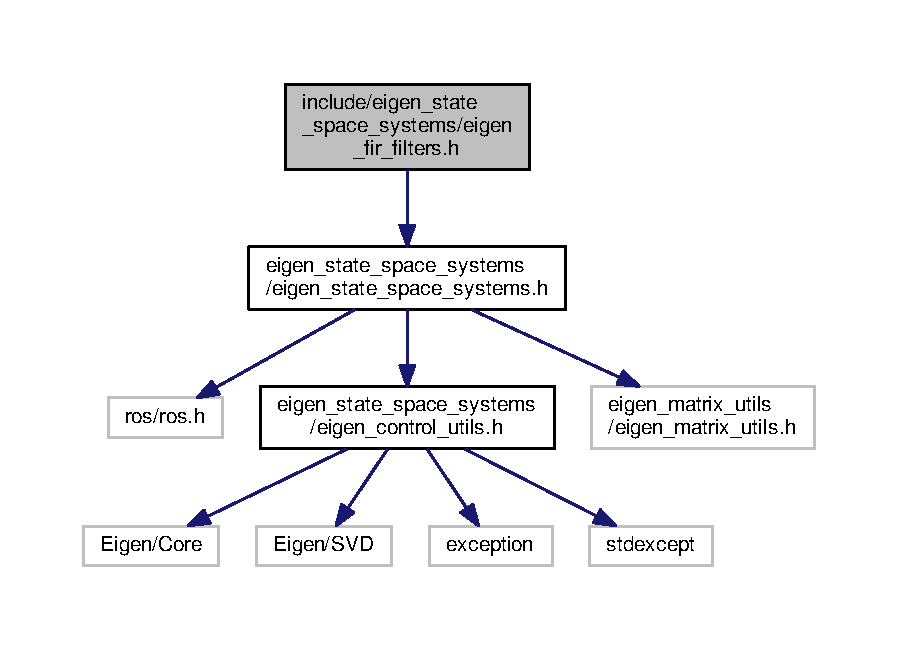
\includegraphics[width=350pt]{eigen__fir__filters_8h__incl}
\end{center}
\end{figure}
This graph shows which files directly or indirectly include this file\+:
\nopagebreak
\begin{figure}[H]
\begin{center}
\leavevmode
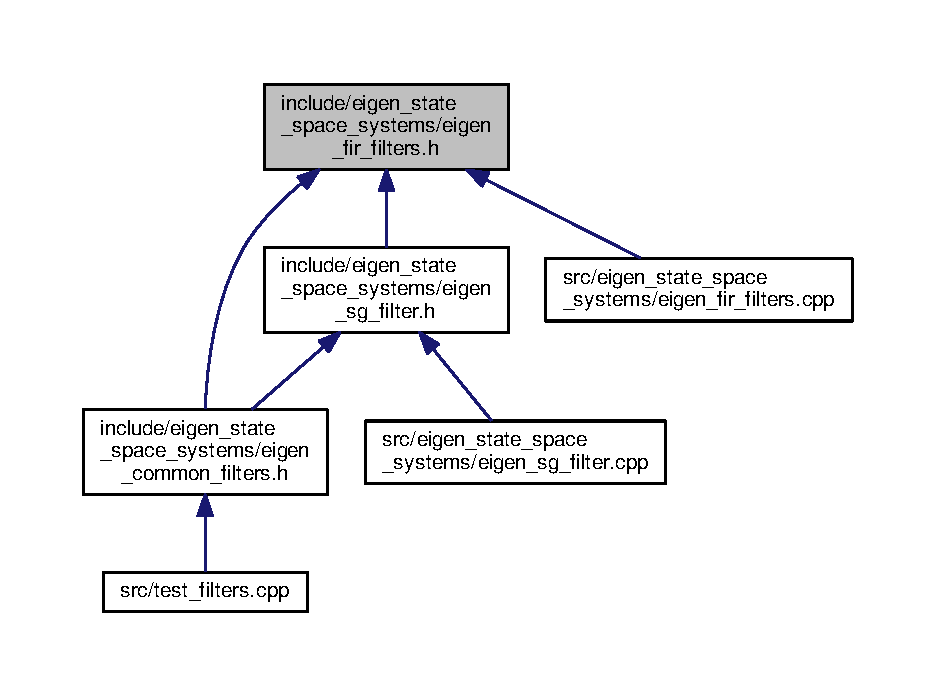
\includegraphics[width=350pt]{eigen__fir__filters_8h__dep__incl}
\end{center}
\end{figure}
\subsection*{Classes}
\begin{DoxyCompactItemize}
\item 
class \hyperlink{classeigen__control__toolbox_1_1_fir_filter}{eigen\+\_\+control\+\_\+toolbox\+::\+Fir\+Filter}
\end{DoxyCompactItemize}
\subsection*{Namespaces}
\begin{DoxyCompactItemize}
\item 
 \hyperlink{namespaceeigen__control__toolbox}{eigen\+\_\+control\+\_\+toolbox}
\end{DoxyCompactItemize}

\hypertarget{eigen__iir__filters_8h}{}\section{include/eigen\+\_\+state\+\_\+space\+\_\+systems/eigen\+\_\+iir\+\_\+filters.h File Reference}
\label{eigen__iir__filters_8h}\index{include/eigen\+\_\+state\+\_\+space\+\_\+systems/eigen\+\_\+iir\+\_\+filters.\+h@{include/eigen\+\_\+state\+\_\+space\+\_\+systems/eigen\+\_\+iir\+\_\+filters.\+h}}
{\ttfamily \#include $<$eigen\+\_\+state\+\_\+space\+\_\+systems/eigen\+\_\+state\+\_\+space\+\_\+systems.\+h$>$}\\*
Include dependency graph for eigen\+\_\+iir\+\_\+filters.\+h\+:
\nopagebreak
\begin{figure}[H]
\begin{center}
\leavevmode
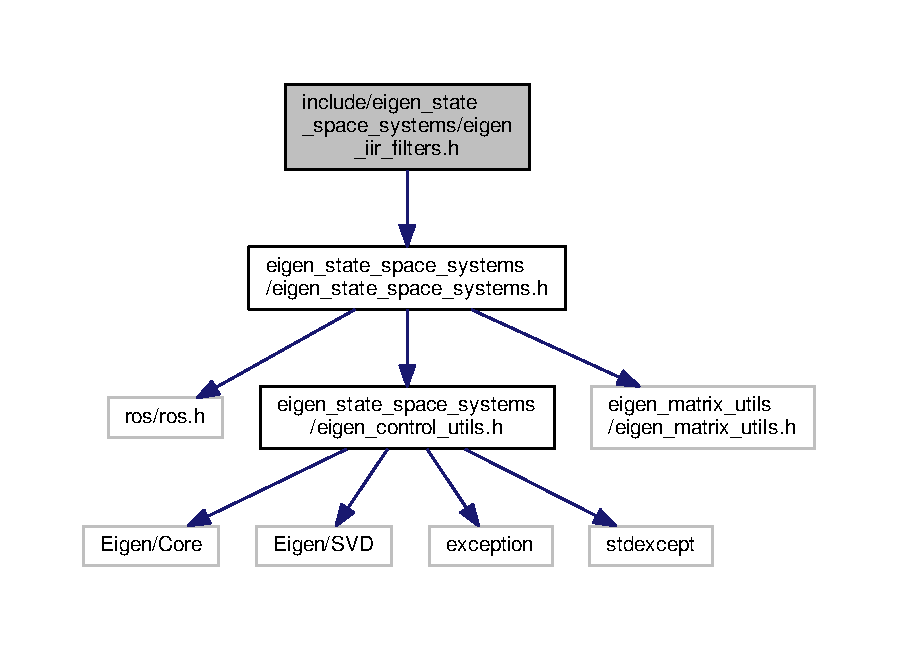
\includegraphics[width=350pt]{eigen__iir__filters_8h__incl}
\end{center}
\end{figure}
This graph shows which files directly or indirectly include this file\+:
\nopagebreak
\begin{figure}[H]
\begin{center}
\leavevmode
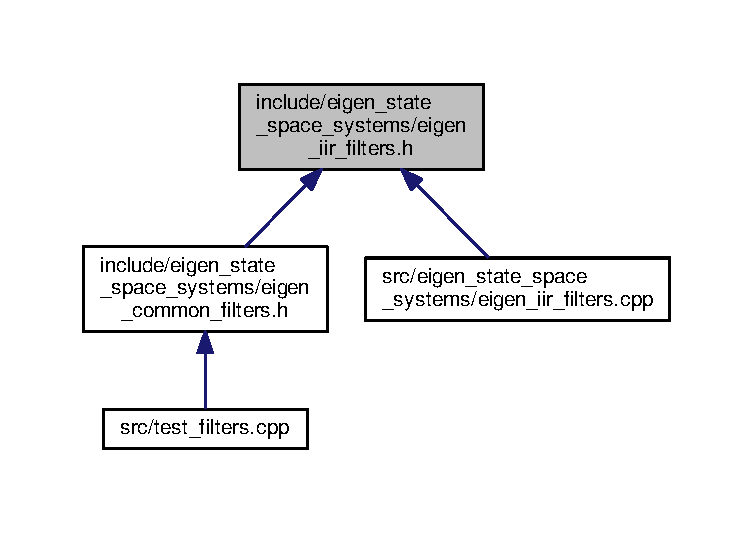
\includegraphics[width=350pt]{eigen__iir__filters_8h__dep__incl}
\end{center}
\end{figure}
\subsection*{Classes}
\begin{DoxyCompactItemize}
\item 
class \hyperlink{classeigen__control__toolbox_1_1_first_order_low_pass}{eigen\+\_\+control\+\_\+toolbox\+::\+First\+Order\+Low\+Pass}
\item 
class \hyperlink{classeigen__control__toolbox_1_1_first_order_high_pass}{eigen\+\_\+control\+\_\+toolbox\+::\+First\+Order\+High\+Pass}
\end{DoxyCompactItemize}
\subsection*{Namespaces}
\begin{DoxyCompactItemize}
\item 
 \hyperlink{namespaceeigen__control__toolbox}{eigen\+\_\+control\+\_\+toolbox}
\end{DoxyCompactItemize}

\hypertarget{eigen__sg__filter_8h}{}\section{include/eigen\+\_\+state\+\_\+space\+\_\+systems/eigen\+\_\+sg\+\_\+filter.h File Reference}
\label{eigen__sg__filter_8h}\index{include/eigen\+\_\+state\+\_\+space\+\_\+systems/eigen\+\_\+sg\+\_\+filter.\+h@{include/eigen\+\_\+state\+\_\+space\+\_\+systems/eigen\+\_\+sg\+\_\+filter.\+h}}
{\ttfamily \#include $<$eigen\+\_\+state\+\_\+space\+\_\+systems/eigen\+\_\+fir\+\_\+filters.\+h$>$}\\*
Include dependency graph for eigen\+\_\+sg\+\_\+filter.\+h\+:
\nopagebreak
\begin{figure}[H]
\begin{center}
\leavevmode
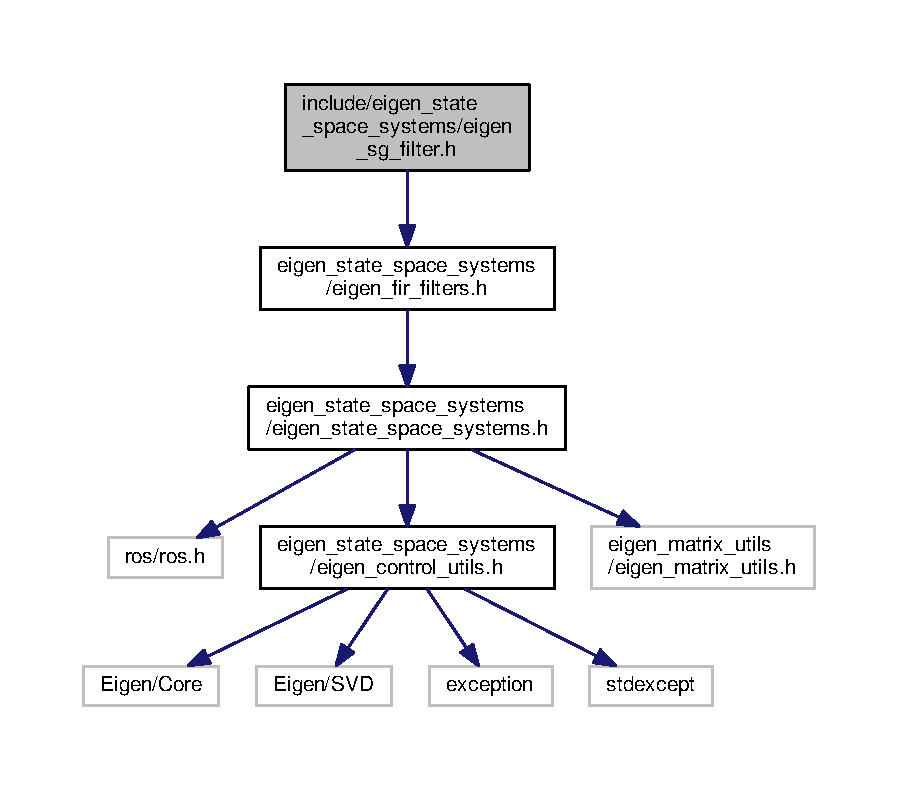
\includegraphics[width=350pt]{eigen__sg__filter_8h__incl}
\end{center}
\end{figure}
This graph shows which files directly or indirectly include this file\+:
\nopagebreak
\begin{figure}[H]
\begin{center}
\leavevmode
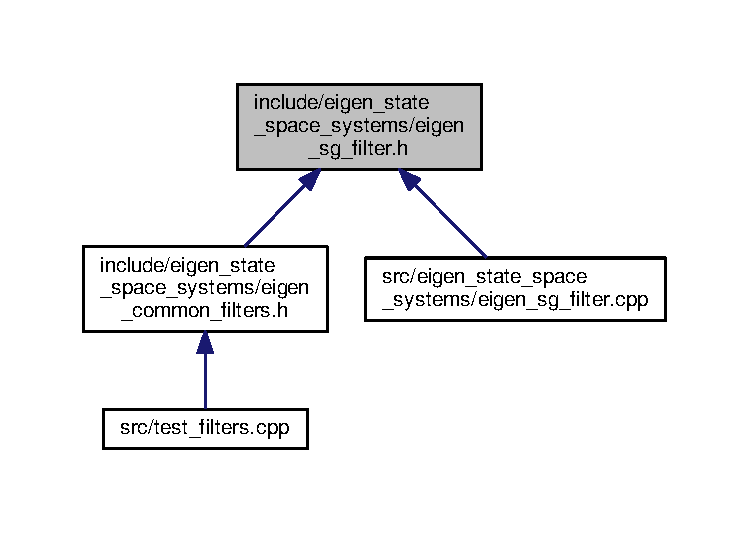
\includegraphics[width=350pt]{eigen__sg__filter_8h__dep__incl}
\end{center}
\end{figure}
\subsection*{Classes}
\begin{DoxyCompactItemize}
\item 
class \hyperlink{classeigen__control__toolbox_1_1_savitky_golay}{eigen\+\_\+control\+\_\+toolbox\+::\+Savitky\+Golay}
\item 
class \hyperlink{classeigen__control__toolbox_1_1_causal_savitky_golay}{eigen\+\_\+control\+\_\+toolbox\+::\+Causal\+Savitky\+Golay}
\end{DoxyCompactItemize}
\subsection*{Namespaces}
\begin{DoxyCompactItemize}
\item 
 \hyperlink{namespaceeigen__control__toolbox}{eigen\+\_\+control\+\_\+toolbox}
\end{DoxyCompactItemize}

\hypertarget{eigen__state__space__systems_8h}{}\section{include/eigen\+\_\+state\+\_\+space\+\_\+systems/eigen\+\_\+state\+\_\+space\+\_\+systems.h File Reference}
\label{eigen__state__space__systems_8h}\index{include/eigen\+\_\+state\+\_\+space\+\_\+systems/eigen\+\_\+state\+\_\+space\+\_\+systems.\+h@{include/eigen\+\_\+state\+\_\+space\+\_\+systems/eigen\+\_\+state\+\_\+space\+\_\+systems.\+h}}
{\ttfamily \#include $<$ros/ros.\+h$>$}\\*
{\ttfamily \#include $<$eigen\+\_\+state\+\_\+space\+\_\+systems/eigen\+\_\+control\+\_\+utils.\+h$>$}\\*
{\ttfamily \#include $<$eigen\+\_\+matrix\+\_\+utils/eigen\+\_\+matrix\+\_\+utils.\+h$>$}\\*
Include dependency graph for eigen\+\_\+state\+\_\+space\+\_\+systems.\+h\+:
\nopagebreak
\begin{figure}[H]
\begin{center}
\leavevmode
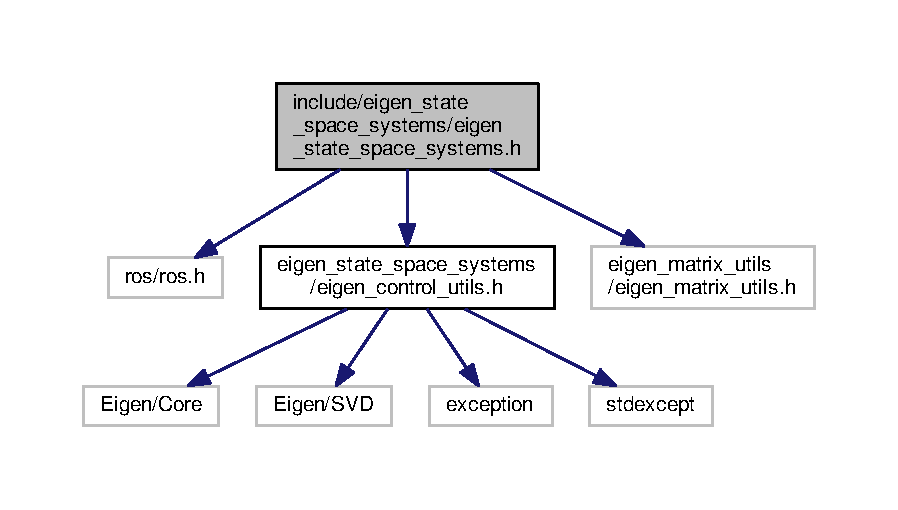
\includegraphics[width=350pt]{eigen__state__space__systems_8h__incl}
\end{center}
\end{figure}
This graph shows which files directly or indirectly include this file\+:
\nopagebreak
\begin{figure}[H]
\begin{center}
\leavevmode
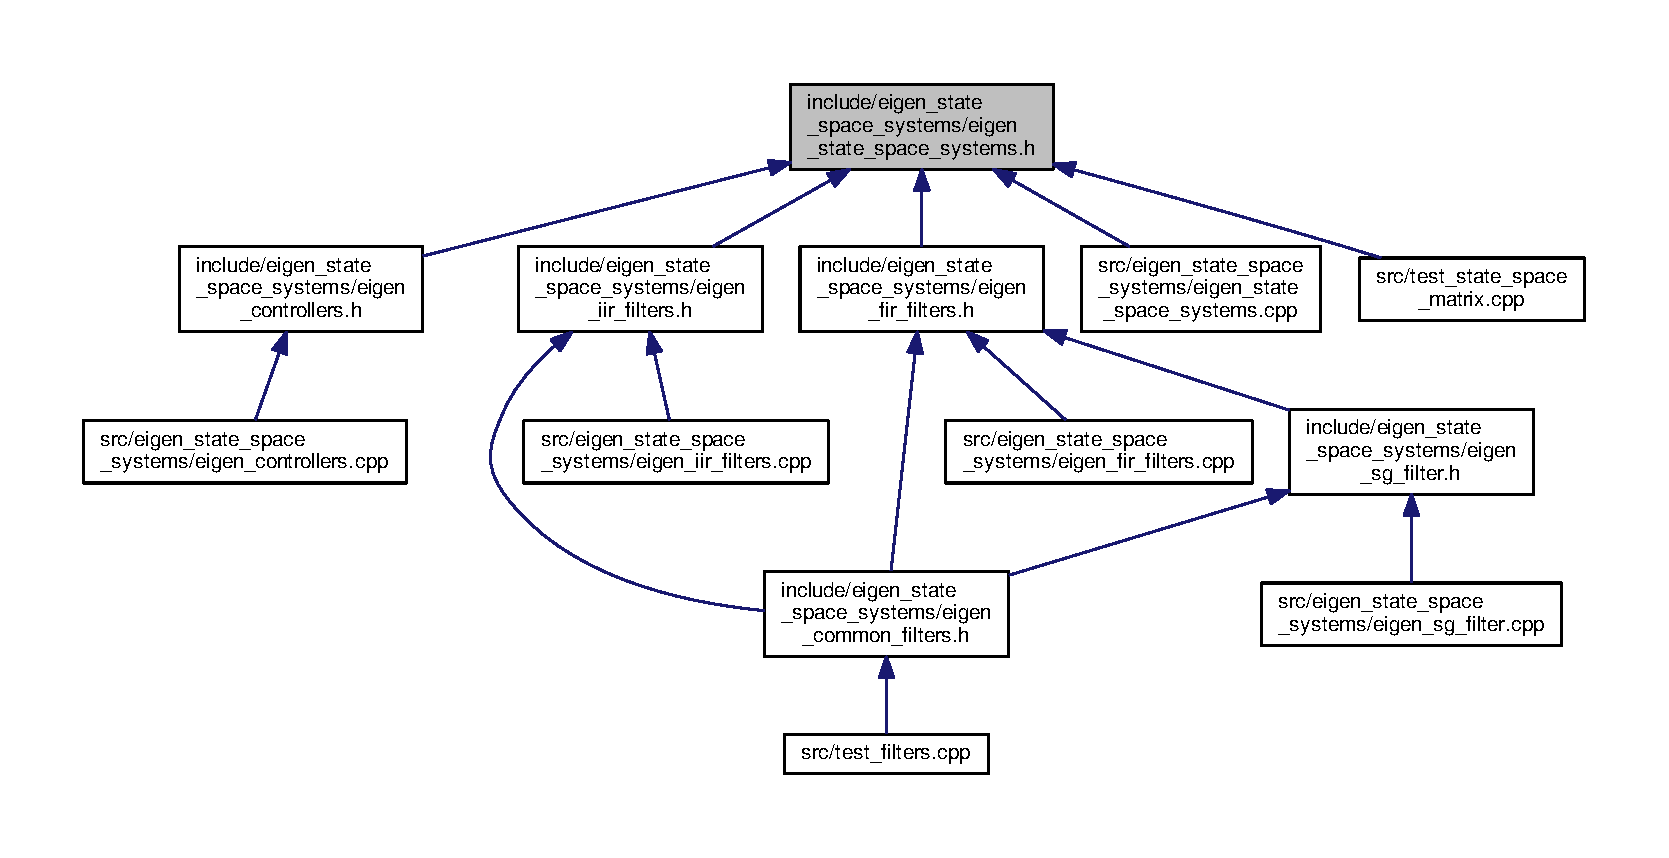
\includegraphics[width=350pt]{eigen__state__space__systems_8h__dep__incl}
\end{center}
\end{figure}
\subsection*{Classes}
\begin{DoxyCompactItemize}
\item 
class \hyperlink{classeigen__control__toolbox_1_1_discrete_state_space}{eigen\+\_\+control\+\_\+toolbox\+::\+Discrete\+State\+Space}
\end{DoxyCompactItemize}
\subsection*{Namespaces}
\begin{DoxyCompactItemize}
\item 
 \hyperlink{namespaceeigen__control__toolbox}{eigen\+\_\+control\+\_\+toolbox}
\end{DoxyCompactItemize}

\hypertarget{eigen__controllers_8cpp}{}\section{src/eigen\+\_\+state\+\_\+space\+\_\+systems/eigen\+\_\+controllers.cpp File Reference}
\label{eigen__controllers_8cpp}\index{src/eigen\+\_\+state\+\_\+space\+\_\+systems/eigen\+\_\+controllers.\+cpp@{src/eigen\+\_\+state\+\_\+space\+\_\+systems/eigen\+\_\+controllers.\+cpp}}
{\ttfamily \#include $<$eigen\+\_\+state\+\_\+space\+\_\+systems/eigen\+\_\+controllers.\+h$>$}\\*
Include dependency graph for eigen\+\_\+controllers.\+cpp\+:
\nopagebreak
\begin{figure}[H]
\begin{center}
\leavevmode
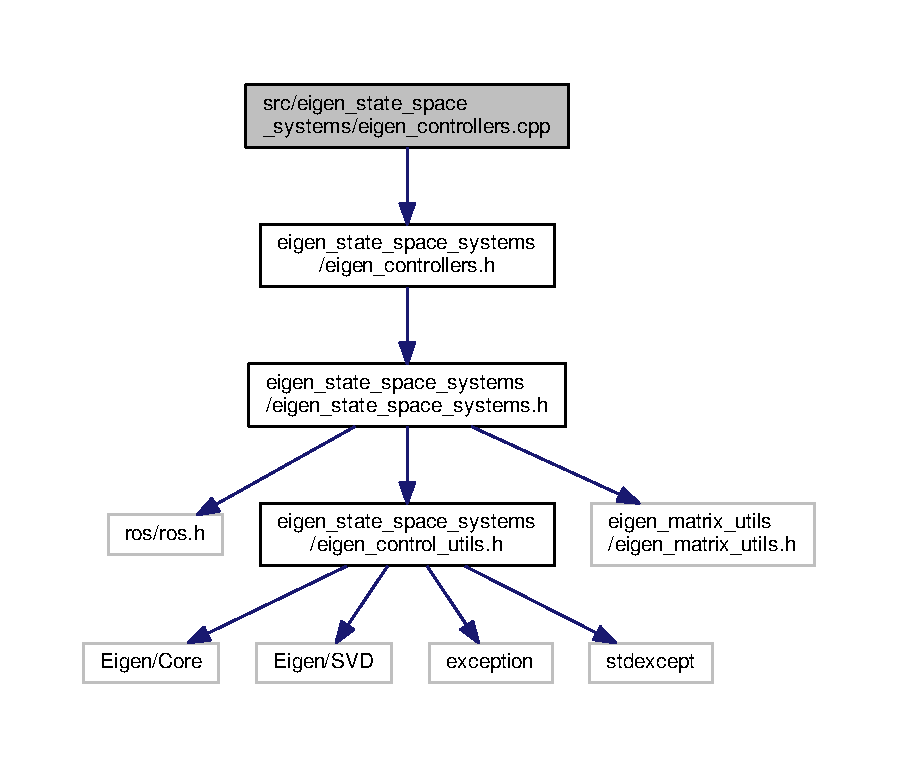
\includegraphics[width=350pt]{eigen__controllers_8cpp__incl}
\end{center}
\end{figure}
\subsection*{Namespaces}
\begin{DoxyCompactItemize}
\item 
 \hyperlink{namespaceeigen__control__toolbox}{eigen\+\_\+control\+\_\+toolbox}
\end{DoxyCompactItemize}

\hypertarget{eigen__fir__filters_8cpp}{}\section{src/eigen\+\_\+state\+\_\+space\+\_\+systems/eigen\+\_\+fir\+\_\+filters.cpp File Reference}
\label{eigen__fir__filters_8cpp}\index{src/eigen\+\_\+state\+\_\+space\+\_\+systems/eigen\+\_\+fir\+\_\+filters.\+cpp@{src/eigen\+\_\+state\+\_\+space\+\_\+systems/eigen\+\_\+fir\+\_\+filters.\+cpp}}
{\ttfamily \#include $<$eigen\+\_\+state\+\_\+space\+\_\+systems/eigen\+\_\+fir\+\_\+filters.\+h$>$}\\*
Include dependency graph for eigen\+\_\+fir\+\_\+filters.\+cpp\+:
\nopagebreak
\begin{figure}[H]
\begin{center}
\leavevmode
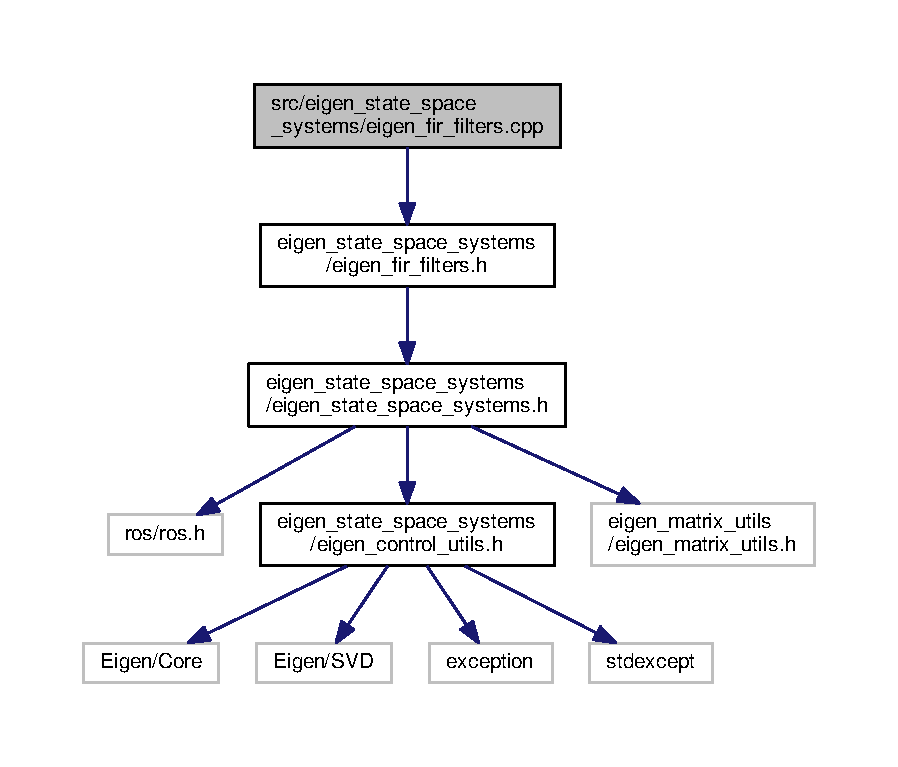
\includegraphics[width=350pt]{eigen__fir__filters_8cpp__incl}
\end{center}
\end{figure}
\subsection*{Namespaces}
\begin{DoxyCompactItemize}
\item 
 \hyperlink{namespaceeigen__control__toolbox}{eigen\+\_\+control\+\_\+toolbox}
\end{DoxyCompactItemize}

\hypertarget{eigen__iir__filters_8cpp}{}\section{src/eigen\+\_\+state\+\_\+space\+\_\+systems/eigen\+\_\+iir\+\_\+filters.cpp File Reference}
\label{eigen__iir__filters_8cpp}\index{src/eigen\+\_\+state\+\_\+space\+\_\+systems/eigen\+\_\+iir\+\_\+filters.\+cpp@{src/eigen\+\_\+state\+\_\+space\+\_\+systems/eigen\+\_\+iir\+\_\+filters.\+cpp}}
{\ttfamily \#include $<$eigen\+\_\+state\+\_\+space\+\_\+systems/eigen\+\_\+iir\+\_\+filters.\+h$>$}\\*
Include dependency graph for eigen\+\_\+iir\+\_\+filters.\+cpp\+:
\nopagebreak
\begin{figure}[H]
\begin{center}
\leavevmode
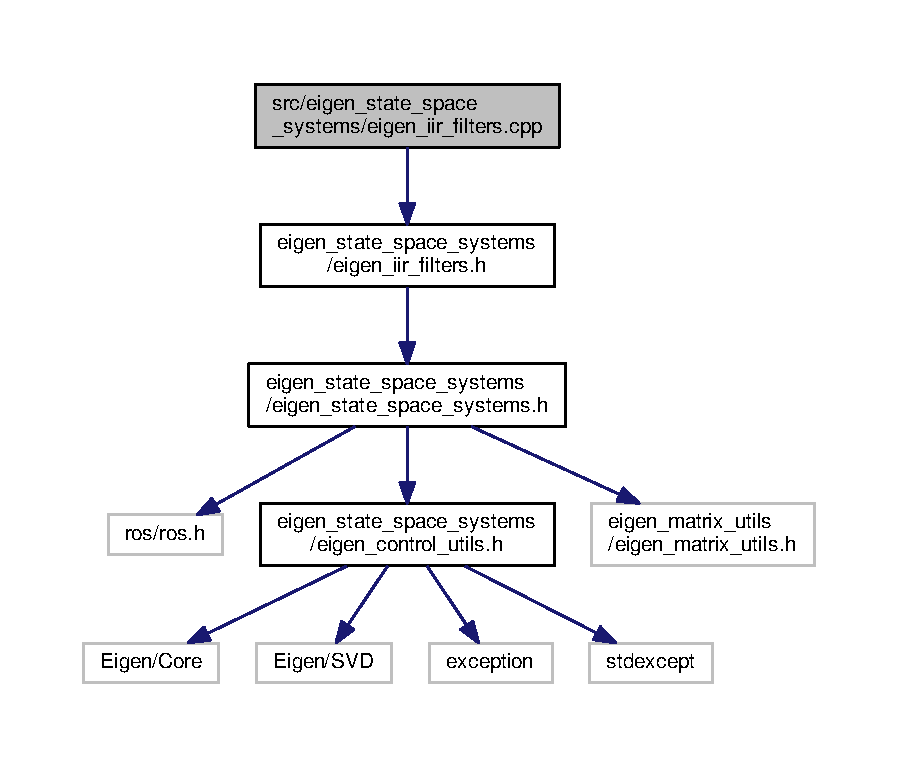
\includegraphics[width=350pt]{eigen__iir__filters_8cpp__incl}
\end{center}
\end{figure}
\subsection*{Namespaces}
\begin{DoxyCompactItemize}
\item 
 \hyperlink{namespaceeigen__control__toolbox}{eigen\+\_\+control\+\_\+toolbox}
\end{DoxyCompactItemize}

\hypertarget{eigen__sg__filter_8cpp}{}\section{src/eigen\+\_\+state\+\_\+space\+\_\+systems/eigen\+\_\+sg\+\_\+filter.cpp File Reference}
\label{eigen__sg__filter_8cpp}\index{src/eigen\+\_\+state\+\_\+space\+\_\+systems/eigen\+\_\+sg\+\_\+filter.\+cpp@{src/eigen\+\_\+state\+\_\+space\+\_\+systems/eigen\+\_\+sg\+\_\+filter.\+cpp}}
{\ttfamily \#include $<$eigen\+\_\+state\+\_\+space\+\_\+systems/eigen\+\_\+sg\+\_\+filter.\+h$>$}\\*
Include dependency graph for eigen\+\_\+sg\+\_\+filter.\+cpp\+:
\nopagebreak
\begin{figure}[H]
\begin{center}
\leavevmode
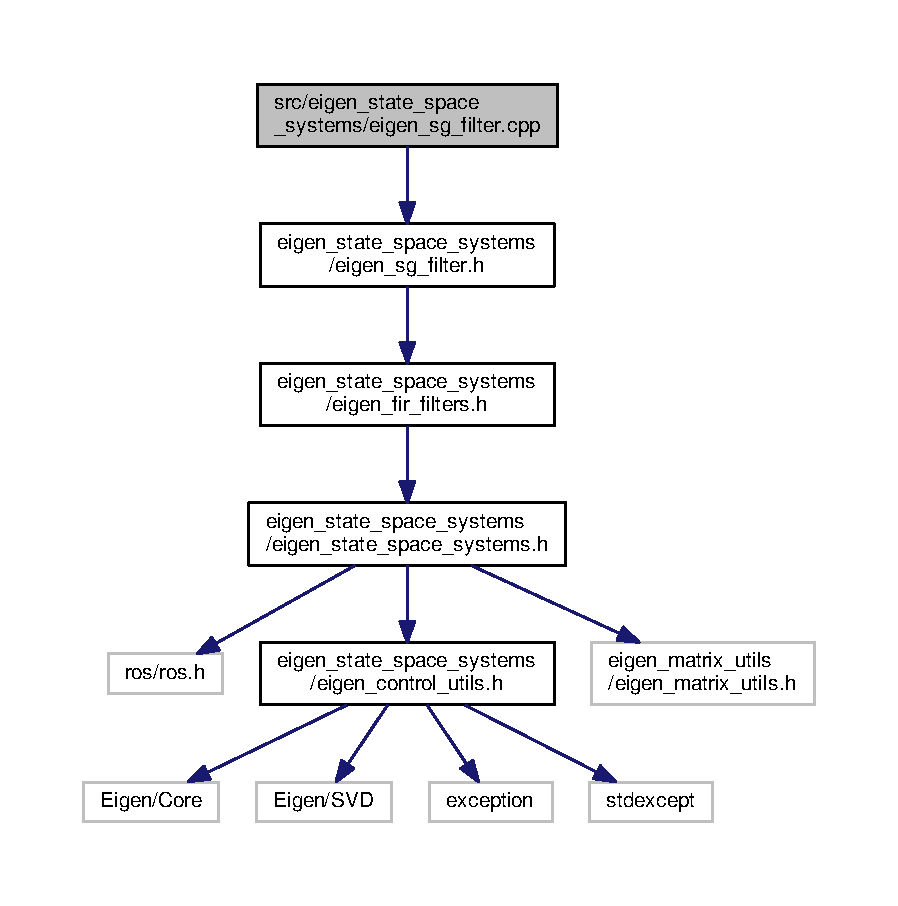
\includegraphics[width=350pt]{eigen__sg__filter_8cpp__incl}
\end{center}
\end{figure}
\subsection*{Namespaces}
\begin{DoxyCompactItemize}
\item 
 \hyperlink{namespaceeigen__control__toolbox}{eigen\+\_\+control\+\_\+toolbox}
\end{DoxyCompactItemize}

\hypertarget{eigen__state__space__systems_8cpp}{}\section{src/eigen\+\_\+state\+\_\+space\+\_\+systems/eigen\+\_\+state\+\_\+space\+\_\+systems.cpp File Reference}
\label{eigen__state__space__systems_8cpp}\index{src/eigen\+\_\+state\+\_\+space\+\_\+systems/eigen\+\_\+state\+\_\+space\+\_\+systems.\+cpp@{src/eigen\+\_\+state\+\_\+space\+\_\+systems/eigen\+\_\+state\+\_\+space\+\_\+systems.\+cpp}}
{\ttfamily \#include $<$eigen\+\_\+state\+\_\+space\+\_\+systems/eigen\+\_\+state\+\_\+space\+\_\+systems.\+h$>$}\\*
{\ttfamily \#include $<$ros/console.\+h$>$}\\*
Include dependency graph for eigen\+\_\+state\+\_\+space\+\_\+systems.\+cpp\+:
\nopagebreak
\begin{figure}[H]
\begin{center}
\leavevmode
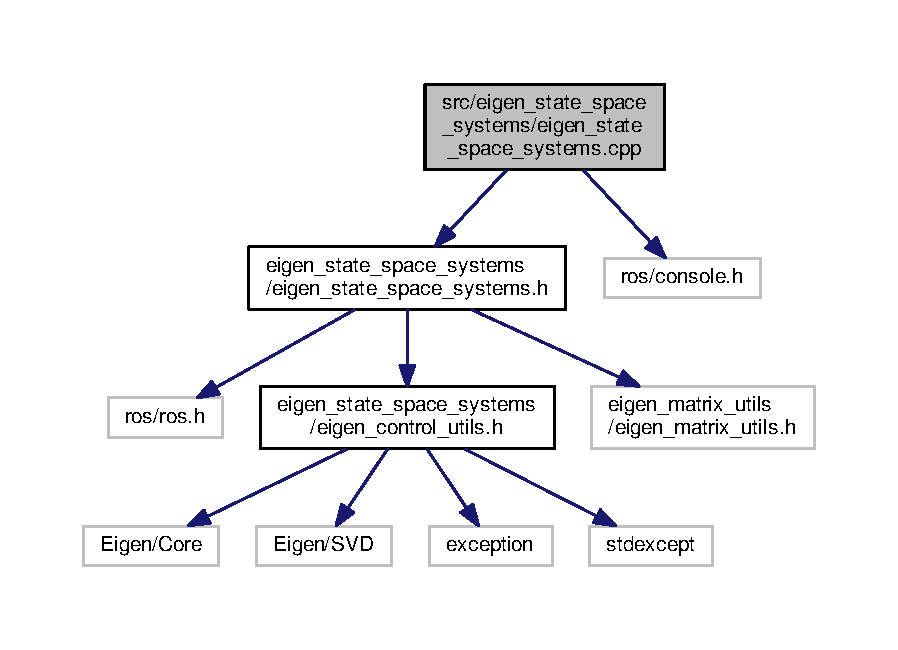
\includegraphics[width=350pt]{eigen__state__space__systems_8cpp__incl}
\end{center}
\end{figure}
\subsection*{Namespaces}
\begin{DoxyCompactItemize}
\item 
 \hyperlink{namespaceeigen__control__toolbox}{eigen\+\_\+control\+\_\+toolbox}
\end{DoxyCompactItemize}

\hypertarget{test__filters_8cpp}{}\section{src/test\+\_\+filters.cpp File Reference}
\label{test__filters_8cpp}\index{src/test\+\_\+filters.\+cpp@{src/test\+\_\+filters.\+cpp}}
{\ttfamily \#include $<$ros/ros.\+h$>$}\\*
{\ttfamily \#include $<$eigen\+\_\+state\+\_\+space\+\_\+systems/eigen\+\_\+common\+\_\+filters.\+h$>$}\\*
{\ttfamily \#include $<$ros/console.\+h$>$}\\*
Include dependency graph for test\+\_\+filters.\+cpp\+:
\nopagebreak
\begin{figure}[H]
\begin{center}
\leavevmode
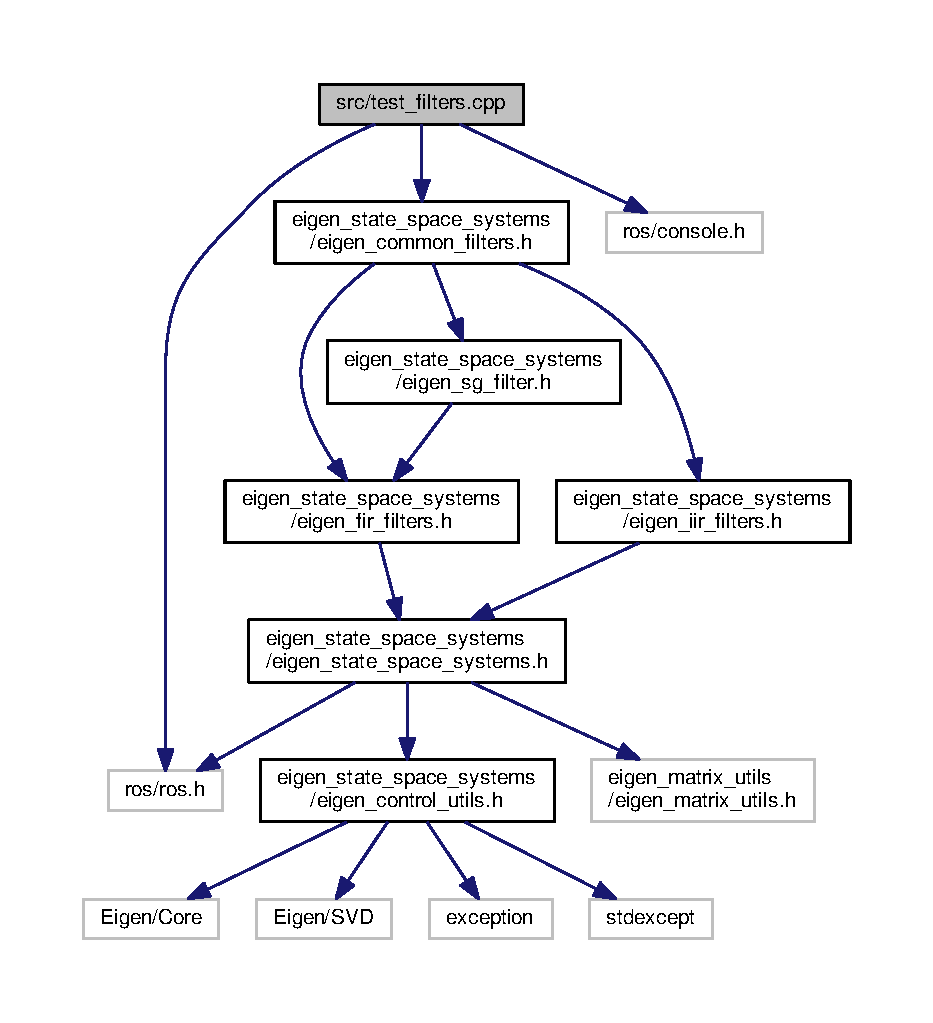
\includegraphics[width=350pt]{test__filters_8cpp__incl}
\end{center}
\end{figure}
\subsection*{Functions}
\begin{DoxyCompactItemize}
\item 
int \hyperlink{test__filters_8cpp_a3c04138a5bfe5d72780bb7e82a18e627}{main} (int argc, char $\ast$$\ast$argv)
\end{DoxyCompactItemize}


\subsection{Function Documentation}
\index{test\+\_\+filters.\+cpp@{test\+\_\+filters.\+cpp}!main@{main}}
\index{main@{main}!test\+\_\+filters.\+cpp@{test\+\_\+filters.\+cpp}}
\subsubsection[{\texorpdfstring{main(int argc, char $\ast$$\ast$argv)}{main(int argc, char **argv)}}]{\setlength{\rightskip}{0pt plus 5cm}int main (
\begin{DoxyParamCaption}
\item[{int}]{argc, }
\item[{char $\ast$$\ast$}]{argv}
\end{DoxyParamCaption}
)}\hypertarget{test__filters_8cpp_a3c04138a5bfe5d72780bb7e82a18e627}{}\label{test__filters_8cpp_a3c04138a5bfe5d72780bb7e82a18e627}


Definition at line 5 of file test\+\_\+filters.\+cpp.


\hypertarget{test__state__space__matrix_8cpp}{}\section{src/test\+\_\+state\+\_\+space\+\_\+matrix.cpp File Reference}
\label{test__state__space__matrix_8cpp}\index{src/test\+\_\+state\+\_\+space\+\_\+matrix.\+cpp@{src/test\+\_\+state\+\_\+space\+\_\+matrix.\+cpp}}
{\ttfamily \#include $<$ros/ros.\+h$>$}\\*
{\ttfamily \#include $<$eigen\+\_\+state\+\_\+space\+\_\+systems/eigen\+\_\+state\+\_\+space\+\_\+systems.\+h$>$}\\*
{\ttfamily \#include $<$ros/console.\+h$>$}\\*
Include dependency graph for test\+\_\+state\+\_\+space\+\_\+matrix.\+cpp\+:
\nopagebreak
\begin{figure}[H]
\begin{center}
\leavevmode
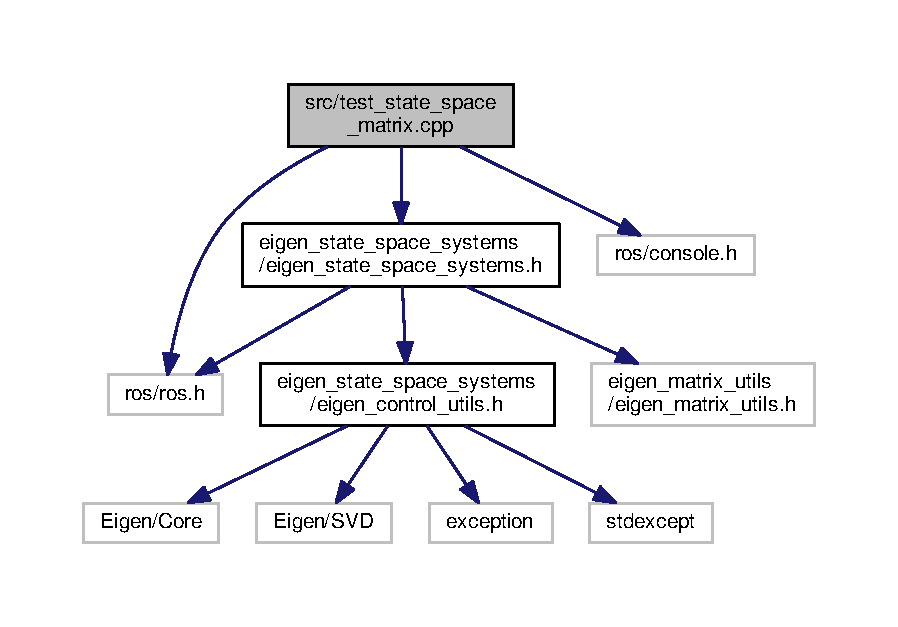
\includegraphics[width=350pt]{test__state__space__matrix_8cpp__incl}
\end{center}
\end{figure}
\subsection*{Functions}
\begin{DoxyCompactItemize}
\item 
int \hyperlink{test__state__space__matrix_8cpp_a3c04138a5bfe5d72780bb7e82a18e627}{main} (int argc, char $\ast$$\ast$argv)
\end{DoxyCompactItemize}


\subsection{Function Documentation}
\index{test\+\_\+state\+\_\+space\+\_\+matrix.\+cpp@{test\+\_\+state\+\_\+space\+\_\+matrix.\+cpp}!main@{main}}
\index{main@{main}!test\+\_\+state\+\_\+space\+\_\+matrix.\+cpp@{test\+\_\+state\+\_\+space\+\_\+matrix.\+cpp}}
\subsubsection[{\texorpdfstring{main(int argc, char $\ast$$\ast$argv)}{main(int argc, char **argv)}}]{\setlength{\rightskip}{0pt plus 5cm}int main (
\begin{DoxyParamCaption}
\item[{int}]{argc, }
\item[{char $\ast$$\ast$}]{argv}
\end{DoxyParamCaption}
)}\hypertarget{test__state__space__matrix_8cpp_a3c04138a5bfe5d72780bb7e82a18e627}{}\label{test__state__space__matrix_8cpp_a3c04138a5bfe5d72780bb7e82a18e627}


Definition at line 5 of file test\+\_\+state\+\_\+space\+\_\+matrix.\+cpp.


%--- End generated contents ---

% Index
\backmatter
\newpage
\phantomsection
\clearemptydoublepage
\addcontentsline{toc}{chapter}{Index}
\printindex

\end{document}
